\documentclass[a4paper,11pt]{book}

% =====================================================
% LANGUAGE AND ENCODING
% =====================================================
\usepackage[utf8]{inputenc}
\usepackage[T1]{fontenc}
\usepackage[italian]{babel}

% =====================================================
% TYPOGRAPHY
% =====================================================
\usepackage{libertinus}
\usepackage[scale=0.95]{sourcesanspro}
\usepackage{microtype}
\usepackage{xcolor}

% =====================================================
% COLOR PALETTE
% =====================================================
\definecolor{Accent}{HTML}{0B3A3E}
\definecolor{TextGray}{gray}{0.25}
\definecolor{RuleGray}{gray}{0.75}
\definecolor{ObsColor}{HTML}{9C5A12}  % ocra scuro, per le osservazioni
\definecolor{FigColor}{HTML}{6B3F73}  % prugna, per le didascalie
\definecolor{LemmaColor}{HTML}{4E7A3A}  % verde foglia, per lemmi, teoremi e corollari
\definecolor{ExColor}{HTML}{4A5560}  % grigio ardesia, per gli esercizi

% =====================================================
% GRAPHICS
% =====================================================
\usepackage{graphicx}
\usepackage{tikz}
\usetikzlibrary{arrows.meta,positioning,decorations.pathreplacing,calc,shapes.multipart,shapes.geometric,fit}

% nodo di un B-diagram: a sinistra la derivata f', a destra la funzione primitiva f
% \node[bnode] (n) {$f'$ \nodepart{two} $f$};
\tikzset{
  bnode/.style={draw, rectangle split, rectangle split horizontal, rectangle split parts=2,
    rounded corners=8pt, minimum height=8mm, inner xsep=5pt, font=\small},
  opnode/.style={draw, circle, minimum size=7mm, inner sep=1pt, font=\small},
  fwd/.style={color=Accent, font=\scriptsize},
  bwd/.style={color=red!70!black, font=\scriptsize},
  flow/.style={-{Stealth[length=2mm]}, thick},
}

% griglie per le convoluzioni (capitolo sulle CNN)
% \numgrid[stile celle]{(x,y)}{lato}{{riga 1},{riga 2},...}: matrice di numeri, (x,y) è lo spigolo in alto a sinistra
% \cellrect[stile]{(x,y)}{lato}{colonna}{riga}{n colonne}{n righe}: rettangolo su un blocco di celle (indici da 0)
% \emptygrid[stile]{(x,y)}{lato}{n colonne}{n righe}: griglia vuota (lato multiplo di 1/8 per evitare errori di arrotondamento)
\newcommand{\numgrid}[4][]{%
  \edef\numgridlist{#4}%
  \foreach \row [count=\ri] in \numgridlist {%
    \foreach \val [count=\ci] in \row {%
      \node[draw=TextGray, minimum size=#3cm, inner sep=0pt, font=\scriptsize, anchor=north west, #1]
        at ($#2 + ({(\ci-1)*#3},{-(\ri-1)*#3})$) {$\val$};
    }%
  }%
}
\newcommand{\cellrect}[7][]{%
  \draw[#1] ($#2 + ({#4*#3},{-#5*#3})$) rectangle ++({#6*#3},{-#7*#3});%
}
\newcommand{\emptygrid}[5][]{%
  \draw[shift={#2}, step=#3cm, #1] (0,0) grid ({#4*#3},{-#5*#3});%
}
\usepackage{subcaption}

% figure interattive della versione web (texweb): nel PDF si stampa la figura statica
\usepackage{texweb}

% =====================================================
% CODE LISTINGS
% =====================================================
\usepackage{listings}
\usepackage[scaled=0.9]{beramono}
\lstdefinestyle{py}{
  language=Python,
  basicstyle=\ttfamily\small,
  numbers=left,
  numbersep=8pt,
  frame=single,
  framerule=0.4pt,
  breaklines=true,
  tabsize=4,
  showstringspaces=false,
  captionpos=b
}

% =====================================================
% MATHEMATICS
% =====================================================
\usepackage{amsmath,amssymb,amsthm}
\numberwithin{equation}{chapter}

% =====================================================
% PAGE LAYOUT
% =====================================================
\usepackage{geometry}
\geometry{a4paper, top=28mm, bottom=30mm, left=30mm, right=30mm}

\usepackage{setspace}
\setstretch{1.12}

\raggedbottom % i box affiancati (esempiofig) non si spezzano: evita pagine stirate
\clubpenalty=10000
\widowpenalty=10000

\setcounter{secnumdepth}{3}
\setcounter{tocdepth}{2}

% =====================================================
% HEADERS AND FOOTERS
% =====================================================
\usepackage{fancyhdr}
\pagestyle{fancy}
\fancyhf{}
\fancyhead[LE,RO]{\thepage}
\fancyhead[LO]{\nouppercase{\rightmark}}
\fancyhead[RE]{\nouppercase{\leftmark}}
\setlength{\headheight}{15pt}
\renewcommand{\headrulewidth}{0.4pt}

% =====================================================
% TABLES
% =====================================================
\usepackage{booktabs}

% =====================================================
% LISTS
% =====================================================
\usepackage{enumitem}
\setlist[itemize]{topsep=4pt, itemsep=3pt}
\setlist[enumerate]{topsep=4pt, itemsep=3pt}
\setlist[description]{font=\normalfont\bfseries, labelsep=0.6em, leftmargin=2em}

% =====================================================
% BOX: DEFINIZIONI E OSSERVAZIONI
% =====================================================
% \begin{definizione}[Titolo opzionale] ... \end{definizione}
%   numerata per capitolo (Definizione 1.1, 1.2, ...), etichettabile con \label
% \begin{esempiofig} testo \tcblower figura \end{esempiofig}
%   esempio con il testo a sinistra e una figura a destra
% \begin{osservazione}[Titolo opzionale] ... \end{osservazione}
%   non numerata, per note, precisazioni e risultati da ricordare
% \begin{lemma}, \begin{esercizio}: si veda più sotto
\usepackage[skins,breakable]{tcolorbox}

\tcbset{
  boxbase/.style={
    enhanced, unbreakable, frame hidden, boxrule=0pt, sharp corners,
    left=12pt, right=10pt, top=7pt, bottom=7pt,
    before skip=0.6em, after skip=0.6em,
    attach title to upper={\ },
    fonttitle=\sffamily\bfseries\small,
    segmentation hidden,
  }
}

% \label dentro i box numerati: usa il numero del box e non quello della sezione
\makeatletter
\newcommand{\tcblabelfix}{\def\@currentlabel{\thetcbcounter}}
\makeatother

\newtcolorbox[auto counter, number within=chapter]{definizione}[1][]{
  boxbase,
  colback=Accent!6, coltitle=Accent,
  borderline west={2.5pt}{0pt}{Accent},
  attach title to upper={\tcblabelfix\ },
  title={Definizione~\thetcbcounter\ifblank{#1}{}{\ (#1)}.},
}

% \begin{lemma}[Titolo opzionale] ... \end{lemma}
%   numerato per capitolo; la dimostrazione si scrive con \paragraph{Dimostrazione.}
\newtcolorbox[auto counter, number within=chapter]{lemma}[1][]{
  boxbase,
  colback=LemmaColor!7, coltitle=LemmaColor,
  borderline west={2.5pt}{0pt}{LemmaColor},
  attach title to upper={\tcblabelfix\ },
  title={Lemma~\thetcbcounter\ifblank{#1}{}{\ (#1)}.},
}

% \begin{teorema}[Titolo opzionale] ... \end{teorema}
% \begin{corollario}[Titolo opzionale] ... \end{corollario}
%   stesso colore del lemma, numerazione separata per capitolo
\newtcolorbox[auto counter, number within=chapter]{teorema}[1][]{
  boxbase,
  colback=LemmaColor!7, coltitle=LemmaColor,
  borderline west={2.5pt}{0pt}{LemmaColor},
  attach title to upper={\tcblabelfix\ },
  title={Teorema~\thetcbcounter\ifblank{#1}{}{\ (#1)}.},
}

\newtcolorbox[auto counter, number within=chapter]{corollario}[1][]{
  boxbase,
  colback=LemmaColor!7, coltitle=LemmaColor,
  borderline west={2.5pt}{0pt}{LemmaColor},
  attach title to upper={\tcblabelfix\ },
  title={Corollario~\thetcbcounter\ifblank{#1}{}{\ (#1)}.},
}

% \begin{esercizio}[Titolo opzionale] testo \end{esercizio}
%   numerato per capitolo (nelle appendici: Esercizio A.1, A.2, ...);
%   la soluzione segue come \paragraph{Soluzione.}
\newtcolorbox[auto counter, number within=chapter]{esercizio}[1][]{
  boxbase,
  colback=ExColor!8, coltitle=ExColor,
  borderline west={2.5pt}{0pt}{ExColor},
  attach title to upper={\tcblabelfix\ },
  title={Esercizio~\thetcbcounter\ifblank{#1}{}{\ (#1)}.},
}

% =====================================================
% DIDASCALIE (stesso stile dei box: sfondo tenue e barra laterale)
% =====================================================
\DeclareCaptionFormat{accentbox}{%
  \begin{tcolorbox}[enhanced, frame hidden, boxrule=0pt, sharp corners,
    colback=FigColor!7, borderline west={2.5pt}{0pt}{FigColor},
    left=12pt, right=10pt, top=6pt, bottom=6pt,
    before skip=0pt, after skip=0pt]
    #1#2#3
  \end{tcolorbox}}
\captionsetup{format=accentbox, labelfont={bf,color=FigColor}, labelsep=period,
  font=small, justification=justified, singlelinecheck=false, skip=8pt}

% esempio con testo a sinistra e figura a destra: \begin{esempiofig} testo \tcblower <figura> \end{esempiofig}
\newtcolorbox{esempiofig}{
  boxbase,
  colback=white, coltitle=black,
  borderline west={1pt}{0pt}{RuleGray},
  title={Esempio.}, fonttitle=\bfseries,
  sidebyside, sidebyside gap=10pt, lefthand ratio=0.52, sidebyside align=center,
  unbreakable,
}

\newtcolorbox{osservazione}[1][]{
  boxbase,
  colback=ObsColor!8, coltitle=ObsColor,
  borderline west={2.5pt}{0pt}{ObsColor},
  title={Osservazione\ifblank{#1}{}{\ (#1)}.},
}

% =====================================================
% MULTICOLUMN
% =====================================================
\usepackage{multicol}

% =====================================================
% ALGORITHMS
% =====================================================
\usepackage{algorithm}
\usepackage{algpseudocode}

% =====================================================
% LINKS
% =====================================================
\usepackage{xurl}
\usepackage[hidelinks]{hyperref}

% =====================================================
% BIBLIOGRAPHY
% =====================================================
\usepackage{csquotes}
\usepackage[backend=bibtex]{biblatex}
\addbibresource{refs.bib}

% =====================================================
% COVER BACKGROUND PATTERN
% =====================================================
\newcommand{\DataPattern}{
  \begin{tikzpicture}[remember picture,overlay]
    \foreach \x in {0.12,0.22,...,0.88} {
      \foreach \y in {0.10,0.20,...,0.90} {
        \fill[Accent!7] ($(current page.south west) + (\x\paperwidth,\y\paperheight)$)
          circle[radius=0.55pt];
      }
    }
    \draw[Accent!10,line width=0.6pt]
      ($(current page.south west)+(0.06\paperwidth,0.30\paperheight)$)
      .. controls ($(current page.south west)+(0.35\paperwidth,0.55\paperheight)$)
      and ($(current page.south west)+(0.55\paperwidth,0.20\paperheight)$)
      .. ($(current page.south west)+(0.92\paperwidth,0.48\paperheight)$);
  \end{tikzpicture}
}

% =====================================================
% METADATA
% =====================================================
\newcommand{\BookTitle}{Riassunti e Appunti di Deep Learning}
\newcommand{\BookSubtitle}{Appunti di corso}
\newcommand{\BookAuthor}{Emanuele Galiano}
\newcommand{\BookUni}{Università degli Studi di Catania}
\newcommand{\BookDept}{Dipartimento di Matematica e Informatica}
\newcommand{\BookAY}{Anno Accademico 2026/2027}
\newcommand{\BookLogoPath}{images/unict_logo.jpg}

% =====================================================
% DOCUMENT
% =====================================================
\begin{document}

\frontmatter

% =====================================================
% TITLE PAGE
% =====================================================
\begin{titlepage}
\thispagestyle{empty}
\DataPattern

\begin{center}
\vspace*{18mm}

{\fontsize{28}{34}\selectfont\bfseries\color{Accent} \BookTitle\par}

\vspace{7mm}
{\color{Accent}\rule{0.66\textwidth}{1.1pt}}

\vspace{10mm}
{\Large\sffamily\color{TextGray}\BookSubtitle\par}

\vspace{20mm}
\includegraphics[height=16mm]{\BookLogoPath}

\vspace{12mm}
{\sffamily\color{TextGray}
\BookUni\\[1mm]
\BookDept\\[1mm]
Corso di Laurea Triennale in Informatica (L-31)
\par}

\vfill

\begin{minipage}{0.92\textwidth}
\sffamily\small\color{TextGray}

% --- Autore (unica colonna) ---
\begin{flushleft}
\textbf{\color{Accent}Autore}\\
\BookAuthor
\end{flushleft}

\vspace{4mm}
{\color{RuleGray}\rule{\textwidth}{0.4pt}}

\vspace{4mm}
\begin{flushleft}
\textbf{\color{Accent}Anno accademico}\\
\BookAY

\vspace{2mm}
\footnotesize
Versione: \today
\end{flushleft}

\end{minipage}

\vspace*{6mm}
\end{center}
\end{titlepage}

% =====================================================
% PREFAZIONE E LICENZA
% =====================================================
\chapter*{Prefazione}

\setlength{\parskip}{0.8em}
\setlength{\parindent}{0pt}

% TODO: inserire il nome del docente del corso.
Queste dispense sono nate come appunti personali per il corso di \emph{Deep Learning} tenuto presso il Dipartimento di Matematica e Informatica dell'Universit\`a di Catania dal Prof. \textbf{[Nome docente]} nell'anno accademico 2026/2027. L'obiettivo principale di questo materiale è stato fornire una risorsa personale di studio sulla parte teorica del corso, raggruppando concetti chiave, definizioni, teoremi, immagini ed esempi in un unico documento, e integrando gli appunti presi a lezione con le slide fornite dal docente.

Questo file non deve essere visto come un testo ufficiale o completo sull'argomento, in quanto potrebbero esserci errori, omissioni o imprecisioni. Invito pertanto chi legge questo documento a consultare le dispense ufficiali del corso proposte dal docente ed eventuali testi di riferimento consigliati. Inoltre, invito chiunque noti errori o abbia suggerimenti a contattarmi via email:
\begin{itemize}
    \item \textbf{Email personale}: \href{mailto:galianoo.emanuele@gmail.com}{galianoo.emanuele@gmail.com},
    \item \textbf{Email universitaria}: \href{mailto:emanuele.galiano@studium.unict.it}{emanuele.galiano@studium.unict.it};
\end{itemize}

\noindent
oppure se ancora presente online, aprire una \textbf{issue} o una \textbf{pull request} nel repository GitHub associato a queste dispense:
\begin{center}
\begin{minipage}{0.92\textwidth}
\centering
\url{https://github.com/emanuelegaliano/Deep-Learning}
\end{minipage}
\end{center}

In particolare, all'interno del repository GitHub sono presenti il codice open-source dei sorgenti \LaTeX{} utilizzati per generare queste dispense, oltre a tutti i file di supporto come immagini e codici per la generazione di alcuni grafici presenti nel testo.

% =====================================================
% LICENSE
% =====================================================
\chapter*{Licenza}
\addcontentsline{toc}{chapter}{Licenza}

\setlength{\parskip}{0.8em}
\setlength{\parindent}{0pt}

Questo documento, intitolato \emph{\BookTitle\ -- \BookSubtitle},
è distribuito sotto licenza \textbf{Creative Commons Attribution-ShareAlike 4.0
International (CC BY-SA 4.0)}.

\noindent
La presente licenza è stata scelta con l'obiettivo di favorire la diffusione,
la condivisione e il riutilizzo del materiale didattico, garantendo al contempo
il riconoscimento degli autori originali e la preservazione della natura open
delle opere derivate.

\vspace{0.6em}

\noindent
\sffamily\small\color{TextGray}
\textbf{Autore:} \BookAuthor \\
\textbf{Affiliazione:} \BookUni\ -- \BookDept \\
\textbf{Anno accademico:} 2026/2027\par
\normalfont\normalsize\color{black}

\vspace{1em}

\section*{Diritti concessi}
\addcontentsline{toc}{section}{Diritti concessi}

In conformità con i termini della licenza Creative Commons BY-SA 4.0, è consentito
a chiunque di:
\begin{itemize}
  \item copiare e ridistribuire il materiale in qualsiasi mezzo o formato;
  \item adattare, modificare e trasformare il materiale;
  \item utilizzare il materiale anche per scopi commerciali.
\end{itemize}

Tali diritti sono concessi a titolo gratuito e non possono essere revocati,
purché siano rispettate le condizioni indicate nella sezione seguente.

\vspace{1em}

\section*{Condizioni}
\addcontentsline{toc}{section}{Condizioni}

L'utilizzo del materiale è subordinato al rispetto delle seguenti condizioni:

\begin{itemize}
  \item \textbf{Attribuzione (BY):} deve essere fornita un'adeguata attribuzione
  dell'opera, citando \textbf{titolo}, \textbf{autori} e, ove possibile, la \textbf{fonte}.
  L'attribuzione deve essere effettuata in modo ragionevole e non tale da suggerire
  che gli autori originali approvino l'uso o le modifiche apportate.

  \item \textbf{Condividi allo stesso modo (SA):} nel caso in cui il materiale
  venga modificato, trasformato o utilizzato per creare opere derivate, tali opere
  devono essere distribuite sotto la \emph{stessa licenza} Creative Commons
  Attribution-ShareAlike 4.0 International.
\end{itemize}

Non è consentito applicare termini legali o misure tecnologiche che limitino
giuridicamente altri utenti nell'esercitare i diritti concessi dalla licenza.

\vspace{1em}

\section*{Assenza di garanzia}
\addcontentsline{toc}{section}{Assenza di garanzia}

Il materiale è fornito \emph{``così com'è''}, senza garanzie di alcun tipo,
esplicite o implicite. In particolare, gli autori non garantiscono l'accuratezza,
la completezza o l'assenza di errori nel contenuto del documento e declinano
ogni responsabilità per eventuali danni derivanti dall'uso del materiale.

\vspace{1em}

\section*{Testo completo della licenza}
\addcontentsline{toc}{section}{Testo completo della licenza}

Il testo legale completo della licenza Creative Commons Attribution-ShareAlike
4.0 International è disponibile al seguente indirizzo:
\begin{center}
\begin{minipage}{0.9\textwidth}
\centering
\url{https://creativecommons.org/licenses/by-sa/4.0/}
\end{minipage}
\end{center}

\vspace{1em}

\noindent
Copyright \textcopyright\ 2026 \\ \BookAuthor

\setlength{\parskip}{0pt}
\setlength{\parindent}{15pt}

% =====================================================
% TOC
% =====================================================
\tableofcontents
\cleardoublepage

% =====================================================
% MAIN CONTENT
% =====================================================
\mainmatter

\part{Core Models and Methods}
\chapter{Ripasso: dal Machine Learning alle reti neurali}\label{ch:ripasso}
Il Deep Learning non nasce dal nulla: le reti neurali profonde riutilizzano quasi tutti gli strumenti già visti nel Machine Learning classico, ovvero un modello parametrico, una funzione di loss da minimizzare, la discesa del gradiente e la regolarizzazione. In questo capitolo riprendiamo questi strumenti partendo dalla regressione logistica e dal modello softmax, mostriamo che il softmax può già essere visto come una rete neurale molto semplice e arriviamo, attraverso il problema della rappresentazione dei dati, al Multi-Layer Perceptron. Il capitolo si chiude con la domanda che motiva tutto il capitolo successivo: come si calcolano i gradienti di una rete con uno o più hidden layer?

\section{Gli ingredienti di un algoritmo di Machine Learning}
Qualunque algoritmo di Machine Learning supervisionato che vedremo è costruito a partire dagli stessi elementi:
\begin{itemize}
    \item \textbf{Un modello}: una funzione $h_\vartheta$ che, dato un input $x$, restituisce una predizione.
    \item \textbf{Dei parametri}: il vettore (o la matrice) $\vartheta$ che determina il comportamento del modello e che va appreso dai dati.
    \item \textbf{Un set di dati}: il training set $\mathcal{D} = \{(x^{(1)}, y^{(1)}), \dots, (x^{(m)}, y^{(m)})\}$, composto da $m$ esempi etichettati.
    \item \textbf{Un algoritmo di learning}: la procedura che, minimizzando una funzione di costo $J(\vartheta)$, trova i parametri migliori per il modello.
\end{itemize}

Ogni input $x^{(i)}$ è un vettore di $n$ feature. Per semplificare la notazione si aggiunge in testa una feature fittizia $x_0^{(i)} = 1$, detta \textbf{bias}, in modo che il termine noto del modello possa essere trattato come un parametro qualunque:
\[
x^{(i)} = \begin{bmatrix} x_0^{(i)} \\ x_1^{(i)} \\ \vdots \\ x_n^{(i)} \end{bmatrix} \in \mathbb{R}^{n+1}, \qquad x_0^{(i)} = 1
\]
dove $x_1^{(i)}, \dots, x_n^{(i)}$ sono le feature vere e proprie dell'$i$-esimo esempio.

\paragraph{Discesa del gradiente.}
Come algoritmo di learning useremo quasi sempre la \textbf{discesa del gradiente}, ovvero un metodo iterativo che aggiorna i parametri nella direzione opposta al gradiente della funzione di costo:
\[
\vartheta_j \leftarrow \vartheta_j - \alpha \frac{\partial J(\vartheta)}{\partial \vartheta_j} \qquad \forall j \text{ simultaneamente}
\]
dove $\alpha > 0$ è il \textbf{learning rate}, un iperparametro che controlla l'ampiezza del passo. Valori tipici si scelgono su una scala approssimativamente logaritmica, ad esempio $0.1,\ 0.03,\ 0.01,\ 0.003,\ 0.001$: un $\alpha$ troppo grande rischia di far divergere l'algoritmo, mentre uno troppo piccolo rende la convergenza molto lenta.

\paragraph{Regolarizzazione.}
L'overfitting è uno dei problemi che si possono incontrare durante il training di un modello. Per contrastarlo si aggiunge alla funzione di costo un \textbf{termine di regolarizzazione}, che penalizza parametri di valore elevato:
\[
J(\vartheta) = \underbrace{-\frac{1}{m}\Big[\cdots\Big]}_{\text{loss sui dati}} + \underbrace{\frac{\lambda}{2m}\sum_{j=1}^{n}\vartheta_j^2}_{\text{regolarizzazione}}
\]
dove $\lambda$ controlla l'intensità della penalizzazione e, tipicamente, il parametro del bias $\vartheta_0$ non viene regolarizzato. Un $\lambda$ grande porta a modelli più semplici, ma se è troppo grande il modello rischia di andare in underfitting.

\section{Regressione logistica}
La \textbf{regressione logistica} è il framework di learning per distinguere tra due classi, ovvero per la classificazione binaria con $y^{(i)} \in \{0, 1\}$. Il modello applica la funzione \textbf{sigmoide} a una combinazione lineare delle feature:
\[
h_\vartheta(x) = \sigma(\vartheta^T x) = \frac{1}{1 + e^{-\vartheta^T x}}, \qquad \vartheta = [\vartheta_0, \vartheta_1, \dots, \vartheta_n]^T \in \mathbb{R}^{n+1}
\]
e restituisce quindi un valore in $(0, 1)$, interpretabile come la probabilità $P(y = 1 \mid x)$.

La funzione di costo è la \textbf{cross-entropy loss} (o binary cross-entropy):
\[
J(\vartheta) = -\frac{1}{m}\sum_{i=1}^{m}\Big[y^{(i)}\log h_\vartheta(x^{(i)}) + (1 - y^{(i)})\log\big(1 - h_\vartheta(x^{(i)})\big)\Big]
\]
che penalizza fortemente le predizioni sicure ma sbagliate: se $y^{(i)} = 1$ e $h_\vartheta(x^{(i)}) \to 0$ (o viceversa) la loss diverge. I parametri si trovano con la discesa del gradiente e, se necessario, con la regolarizzazione vista sopra.

Per eseguire una classificazione multiclasse con la regressione logistica si può ricorrere all'approccio \textbf{one vs all}, addestrando un classificatore binario per ogni classe. Questa strategia presenta però diverse criticità: il numero di classificatori cresce con il numero di classi, possono comparire regioni di incertezza e le probabilità restituite dai singoli classificatori non sono facilmente confrontabili. Per questo motivo si introduce un modello pensato direttamente per il caso multiclasse.

\section{Softmax}\label{sec:softmax}
Il \textbf{softmax} è il framework di learning per eseguire la classificazione multiclasse, ed è un'estensione della regressione logistica. Le etichette appartengono ora a $K$ classi, $y^{(i)} \in \{0, 1, \dots, K-1\}$, e vengono rappresentate con il \textbf{one-hot encoding}, ovvero come un vettore di $K$ componenti tutte nulle tranne quella corrispondente alla classe corretta, che vale 1.

\subsection{Il modello}
Dato un input $x$, vogliamo stimare la probabilità che appartenga a ciascuna delle classi:
\[
P_\vartheta(y = k \mid x) \qquad \forall k = 0, 1, \dots, K-1.
\]
La nostra ipotesi deve quindi stimare un vettore di $K$ probabilità, e per farlo ogni classe $k$ ha il proprio vettore di parametri $\vartheta^{(k)} \in \mathbb{R}^{n+1}$.

\begin{definizione}[Modello softmax]
Il modello softmax restituisce la distribuzione di probabilità sulle $K$ classi:
\[
h_\vartheta(x) =
\begin{bmatrix}
P_\vartheta(y = 0 \mid x) \\ P_\vartheta(y = 1 \mid x) \\ \vdots \\ P_\vartheta(y = K-1 \mid x)
\end{bmatrix}
= \frac{1}{\displaystyle\sum_{k=0}^{K-1} e^{\vartheta^{(k)T} x}}
\begin{bmatrix}
e^{\vartheta^{(0)T} x} \\ e^{\vartheta^{(1)T} x} \\ \vdots \\ e^{\vartheta^{(K-1)T} x}
\end{bmatrix}
\]
ovvero, per la singola classe $c$:
\[
h_\vartheta^{(c)}(x) = P_\vartheta(y = c \mid x) = \frac{e^{\vartheta^{(c)T} x}}{\displaystyle\sum_{k=0}^{K-1} e^{\vartheta^{(k)T} x}}.
\]
\end{definizione}

Il denominatore normalizza la distribuzione, per cui, una volta fissati (appresi) i parametri, la somma delle probabilità restituite è sempre pari a 1:
\[
\sum_{k=0}^{K-1} P_\vartheta(y = k \mid x) = 1.
\]
I parametri del modello non sono più un vettore ma una matrice, in cui la colonna $k$-esima contiene i parametri $\vartheta^{(k)}$ della classe $k$:
\[
\vartheta =
\begin{bmatrix}
\vartheta_0^{(0)} & \vartheta_0^{(1)} & \cdots & \vartheta_0^{(K-1)} \\
\vartheta_1^{(0)} & \vartheta_1^{(1)} & \cdots & \vartheta_1^{(K-1)} \\
\vdots & \vdots & \ddots & \vdots \\
\vartheta_n^{(0)} & \vartheta_n^{(1)} & \cdots & \vartheta_n^{(K-1)}
\end{bmatrix}
\in \mathbb{R}^{(n+1) \times K}.
\]

\subsection{Funzione di costo e learning}
Anche il softmax usa la cross-entropy loss, che confronta il vettore one-hot dell'etichetta con le probabilità uscite dal modello. Per scriverla definiamo la \textbf{funzione indicatrice}:
\[
\mathbf{1}\{\text{proposizione}\} =
\begin{cases}
1 & \text{se la proposizione è vera} \\
0 & \text{se la proposizione è falsa}
\end{cases}
\]
La funzione di costo del softmax è quindi:
\[
J(\vartheta) = -\frac{1}{m}\left[\sum_{i=1}^{m}\sum_{c=0}^{K-1}\mathbf{1}\{y^{(i)} = c\}\log h_\vartheta^{(c)}(x^{(i)})\right] + \underbrace{\frac{\lambda}{2m}\sum_{c=0}^{K-1}\sum_{j=1}^{n}\big(\vartheta_j^{(c)}\big)^2}_{\text{regolarizzazione}}
\]
dove, per ogni esempio, sopravvive solo il termine della classe corretta: la loss è quindi $-\log$ della probabilità assegnata alla classe giusta.

L'obiettivo del learning è trovare i parametri che minimizzano $J(\vartheta)$, cosa che si fa con la discesa del gradiente (o con la sua versione stocastica). La derivata parziale rispetto al generico parametro vale:
\[
\frac{\partial J(\vartheta)}{\partial \vartheta_j^{(c)}} = -\frac{1}{m}\sum_{i=1}^{m}\Big[\big(\mathbf{1}\{y^{(i)} = c\} - h_\vartheta^{(c)}(x^{(i)})\big)\,x_j^{(i)}\Big] + \frac{\lambda}{m}\vartheta_j^{(c)}
\]
e l'aggiornamento viene ripetuto fino a convergenza:
\[
\vartheta_j^{(c)} \leftarrow \vartheta_j^{(c)} - \alpha\frac{\partial J(\vartheta)}{\partial \vartheta_j^{(c)}} \qquad \forall j = 0, \dots, n,\ \forall c = 0, \dots, K-1 \text{ simultaneamente.}
\]

\begin{osservazione}[Gradiente rispetto ai logit]
Chiamiamo \textbf{logit} le quantità $z_k = \vartheta^{(k)T}x$, ovvero i valori prima della normalizzazione. Per un singolo esempio, il gradiente della cross-entropy rispetto a ciascun logit ha una forma molto semplice:
\[
\delta_k = \frac{\partial L}{\partial z_k} = p_k - y_k
\]
dove $p_k$ è la probabilità predetta e $y_k$ la componente $k$-esima del vettore one-hot. Il gradiente rispetto al peso che collega la feature $x_j$ al nodo $k$ è poi semplicemente $\delta_k x_j$, mentre quello rispetto al bias è $\delta_k$. È la stessa espressione della formula precedente, letta nodo per nodo: questa idea di \emph{errore locale} propagato all'indietro tornerà nel capitolo~\ref{ch:backprop}.
\end{osservazione}

\subsection{Overparametrizzazione}
Il modello softmax è \textbf{overparametrizzato}, ovvero, per ogni ipotesi che descrive i dati, esistono infinite configurazioni dei parametri che producono esattamente la stessa mappa dagli input $x$ alle predizioni. Infatti, sottraendo a ogni vettore $\vartheta^{(k)}$ lo stesso vettore arbitrario $\psi \in \mathbb{R}^{n+1}$:
\[
\frac{e^{(\vartheta^{(c)} - \psi)^T x}}{\displaystyle\sum_{k=0}^{K-1} e^{(\vartheta^{(k)} - \psi)^T x}}
= \frac{e^{\vartheta^{(c)T} x}\, e^{-\psi^T x}}{e^{-\psi^T x}\displaystyle\sum_{k=0}^{K-1} e^{\vartheta^{(k)T} x}}
= \frac{e^{\vartheta^{(c)T} x}}{\displaystyle\sum_{k=0}^{K-1} e^{\vartheta^{(k)T} x}}
\]
il fattore comune $e^{-\psi^T x}$ si semplifica e l'ipotesi $h_\vartheta$ non cambia.

\paragraph{Relazione con la regressione logistica.}
Questa proprietà permette di mostrare facilmente che, nel caso particolare $K = 2$, il softmax si riduce alla regressione logistica. Scegliendo $\psi = \vartheta^{(1)}$:
\[
h_\vartheta(x) =
\begin{bmatrix}
\dfrac{e^{(\vartheta^{(0)} - \vartheta^{(1)})^T x}}{e^{(\vartheta^{(0)} - \vartheta^{(1)})^T x} + e^{\mathbf{0}^T x}} \\[12pt]
\dfrac{e^{\mathbf{0}^T x}}{e^{(\vartheta^{(0)} - \vartheta^{(1)})^T x} + e^{\mathbf{0}^T x}}
\end{bmatrix}
=
\begin{bmatrix}
1 - \dfrac{1}{1 + e^{(\vartheta^{(0)} - \vartheta^{(1)})^T x}} \\[12pt]
\dfrac{1}{1 + e^{(\vartheta^{(0)} - \vartheta^{(1)})^T x}}
\end{bmatrix}
\]
dove si è usato $e^{\mathbf{0}^T x} = 1$. La differenza $\vartheta^{(1)} - \vartheta^{(0)}$ può essere sostituita da un unico vettore di parametri $\vartheta$, ottenendo proprio $h_\vartheta^{(1)}(x) = \sigma(\vartheta^T x)$ e $h_\vartheta^{(0)}(x) = 1 - h_\vartheta^{(1)}(x)$. Allo stesso modo, per $K = 2$ e senza regolarizzazione, la funzione di costo del softmax diventa:
\[
J(\vartheta) = -\frac{1}{m}\sum_{i=1}^{m}\Big[(1 - y^{(i)})\log\big(1 - h_\vartheta^{(1)}(x^{(i)})\big) + y^{(i)}\log h_\vartheta^{(1)}(x^{(i)})\Big]
\]
ovvero la cross-entropy della regressione logistica: la regressione logistica è quindi un caso particolare del softmax.

\subsection{Il softmax come rete neurale}
Il softmax segue un modello lineare, tuttavia può essere rappresentato come una rete neurale molto semplice, con un solo layer di pesi tra input e output. I suoi \emph{ingredienti} sono tre:
\begin{enumerate}
    \item \textbf{Modello lineare}: per ogni classe $k$ si calcola $z_k = \vartheta^{(k)T}x$.
    \item \textbf{Logit}: si applica l'esponenziale, $e^{z_k}$.
    \item \textbf{Normalizzazione}: si divide per $\sum_j e^{z_j}$, ottenendo probabilità che sommano a 1.
\end{enumerate}

\begin{figure}[htbp]
\centering
\begin{widget}{softmax}[x={0.2, 0.1}, theta={{-1,1,0},{1,0.5,1},{2,1,1.5}}, target=0]
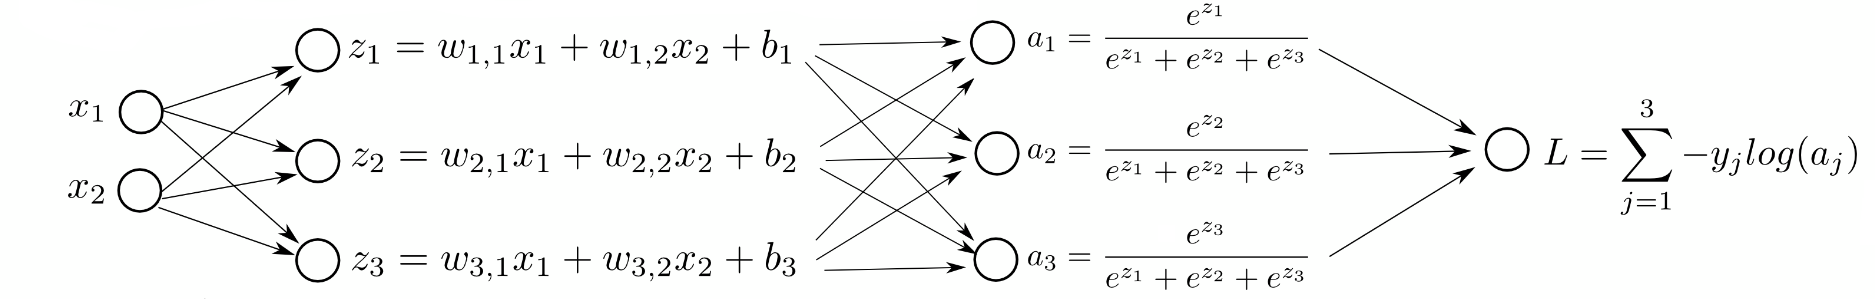
\includegraphics[width=\textwidth]{images/softmax_neural_network.png}
\end{widget}
\caption{Il softmax come rete neurale con due feature e tre classi: dai logit $z_i = w_{i,1}x_1 + w_{i,2}x_2 + b_i$ alle probabilità $a_i = e^{z_i}/\sum_{k=1}^{3}e^{z_k}$, fino alla cross-entropy loss $L = \sum_{j=1}^{3} -y_j\log(a_j)$. Il bias $b_i$ corrisponde al parametro $\vartheta_0^{(i)}$ associato alla feature $x_0 = 1$.}
\label{fig:softmax-nn}
\end{figure}

\paragraph{Esempio.}
Consideriamo tre classi e un input con due feature, $x = [1,\ 0.2,\ 0.1]^T$ (la prima componente è il bias). Siano i parametri, scritti per righe (una riga per classe):
\[
\vartheta^T =
\begin{bmatrix}
-1 & 1 & 0 \\
1 & 0.5 & 1 \\
2 & 1 & 1.5
\end{bmatrix}
\]
e supponiamo che la classe corretta sia la prima, $y = [1, 0, 0]^T$.

\textbf{Soluzione.} Calcoliamo in ordine i tre ingredienti del softmax:
\begin{center}
\begin{tabular}{@{}cccc@{}}
\toprule
Classe & Modello lineare $z_k$ & Logit $e^{z_k}$ & Normalizzazione $p_k$ \\
\midrule
0 & $-1 + 0.2 + 0 = -0.8$ & $0.45$ & $0.03$ \\
1 & $1 + 0.1 + 0.1 = 1.2$ & $3.32$ & $0.23$ \\
2 & $2 + 0.2 + 0.15 = 2.35$ & $10.49$ & $0.74$ \\
\midrule
 & & $\sum = 14.26$ & $\sum = 1$ \\
\bottomrule
\end{tabular}
\end{center}
Il modello assegna alla classe corretta una probabilità di appena $0.03$, per cui la loss su questo campione è alta: $L = -1\cdot\log(0.0315) \approx 3.46$. La loss complessiva si ottiene facendo la media di questi valori su tutti gli $m$ campioni del training set.

\begin{figure}[htbp]
\centering
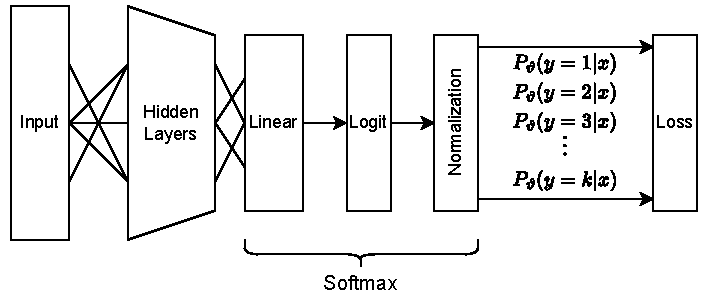
\includegraphics[width=0.85\textwidth]{images/neural-net.pdf}
\caption{Struttura ``standard'' di una rete neurale per la classificazione: dopo l'input e gli hidden layer, gli ultimi blocchi (modello lineare, logit e normalizzazione) sono esattamente un softmax, che produce le probabilità $P_\vartheta(y = k \mid x)$ su cui viene calcolata la loss.}
\label{fig:nn-standard}
\end{figure}

\section{Loss function e Multi-Class SVM}
Ci si potrebbe chiedere se anche una SVM sia una rete neurale. Una SVM lineare, come il softmax, è una \textbf{macchina lineare}: calcola un vettore di punteggi $f = Wx + b$, uno per classe. Ciò che cambia tra i due modelli è soltanto la funzione di loss: cambiando la loss di questo framework lineare si ottiene la \textbf{Multi-Class SVM}, che usa la \textbf{hinge loss}:
\[
L = \underbrace{\frac{1}{N}\sum_{i}\sum_{j \neq y_i}\max(0,\ f_j - f_{y_i} + 1)}_{\text{data loss}} + \underbrace{\lambda\sum_{k}\sum_{l}W_{k,l}^2}_{\text{regularization loss}}
\]
dove $f_{y_i}$ è il punteggio della classe corretta. In questo senso una SVM lineare può essere vista come la stessa rete a un solo layer del softmax, con una loss diversa; tipicamente, però, il termine ``rete neurale'' si riserva a modelli che apprendono anche una rappresentazione degli input, come vedremo tra poco.

\paragraph{Esempio.}
Siano $f = [-2.85,\ 0.86,\ 0.28]^T$ i punteggi prodotti da $Wx + b$ per un esempio la cui classe corretta è $y_i = 2$, ovvero quella con punteggio $0.28$.

\textbf{Soluzione.} Con la hinge loss si sommano i contributi delle classi errate:
\[
L_{\text{hinge}} = \max(0,\ -2.85 - 0.28 + 1) + \max(0,\ 0.86 - 0.28 + 1) = 0 + 1.58 = 1.58.
\]
Con la cross-entropy, invece, si applicano esponenziale e normalizzazione,
\[
e^{f} = [0.058,\ 2.36,\ 1.32]^T \quad\Longrightarrow\quad p = [0.015,\ 0.631,\ 0.353]^T,
\]
e si prende il logaritmo della probabilità della classe corretta: $L_{\text{CE}} = -\log(0.353) \approx 1.04$.

\paragraph{Loss per la classificazione binaria.}
In generale, la loss complessiva è la somma delle loss sui singoli esempi, $L = \sum_{i=1}^{m}\mathrm{loss}\big(f(x^{(i)}), y^{(i)}\big)$. Nel caso binario, con $y^{(i)} \in \{-1, +1\}$, alcuni esempi sono:
\begin{itemize}
    \item \textbf{Zero-one loss}: $\mathbf{1}\{\mathrm{sign}(f(x^{(i)})) \neq y^{(i)}\}$, che conta gli errori ma non è né continua né derivabile.
    \item \textbf{Hinge loss}: $\max\big(0,\ 1 - f(x^{(i)})\,y^{(i)}\big)$, usata dalle SVM.
    \item \textbf{Logistic loss}: $\log\big(1 + \exp(-f(x^{(i)})\,y^{(i)})\big)$, usata dalla regressione logistica.
\end{itemize}
Allo stesso modo, la regressione lineare usa la \textbf{least squares loss} $\frac{1}{2}(y - z)^2$, mentre le reti neurali per la classificazione usano la cross-entropy. In tutti i casi la funzione di costo da minimizzare con la discesa del gradiente è $J(\vartheta) = \sum_{i=1}^{m} L\big(h_\vartheta(x^{(i)}), y^{(i)}\big)$, e il modello restituisce un valore continuo nella regressione o una classe nella classificazione.

\section{Il ruolo della rappresentazione}
Un modello lineare come il softmax produce sempre decision boundary lineari: funziona bene quando i dati sono \textbf{linearmente separabili}, ma fallisce quando non lo sono, come nel caso di due classi disposte a cerchi concentrici. Una soluzione nota è quella di trasformare le feature con una funzione $\phi(x)$, ad esempio un kernel, che mappa i dati in uno spazio a dimensione più alta in cui diventano separabili da un iperpiano (figura~\ref{fig:kernel}).

\begin{figure}[htbp]
\centering
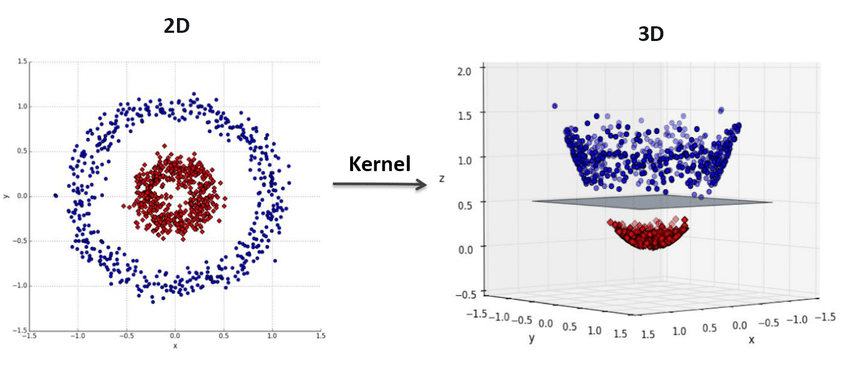
\includegraphics[width=0.75\textwidth]{images/non_linear_SVM.png}
\caption{Dati non linearmente separabili nello spazio di input bidimensionale (a sinistra): due classi disposte a cerchi concentrici. Applicando una trasformazione $\phi$ che aggiunge una dimensione (a destra), le due classi diventano separabili da un piano nello spazio delle feature.}
\label{fig:kernel}
\end{figure}

Il problema è che scegliere la $\phi(x)$ giusta non è semplice: dipende dai dati e dal task, e una rappresentazione costruita a mano (\emph{hand crafted}) potrebbe non essere quella migliore. La domanda diventa allora: possiamo \textbf{apprendere} la funzione $\phi(x)$ direttamente dai dati? La risposta sono le reti neurali e il Deep Learning, che fanno \textbf{representation learning}, ovvero imparano in modo supervisionato, a seconda del task, come trasformare l'input in una rappresentazione utile.

\section{Reti neurali}\label{sec:reti-neurali}
La prima rete neurale studiata fu il \textbf{percettrone} di Rosenblatt, ovvero un singolo neurone che calcola una somma pesata degli input (con la soglia incorporata come peso $\vartheta_0$ del bias $x_0 = 1$) e restituisce un'uscita binaria. Il percettrone è dotato di una procedura di learning automatico dei pesi, ma, come tutti i modelli lineari, risolve solo problemi linearmente separabili: non è in grado, ad esempio, di calcolare lo XOR.

\begin{figure}[htbp]
\centering
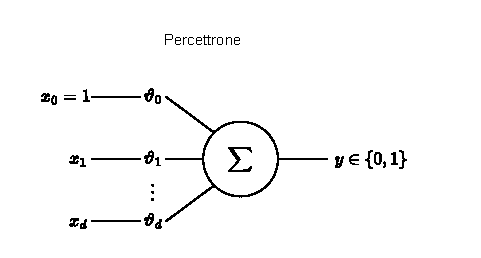
\includegraphics[width=0.5\textwidth]{images/percettrone.pdf}
\caption{Il percettrone di Rosenblatt: le feature $x_1, \dots, x_d$ e il bias $x_0 = 1$ vengono pesati dai parametri $\vartheta_0, \dots, \vartheta_d$ e sommati; l'uscita è binaria, $y \in \{0, 1\}$.}
\label{fig:percettrone}
\end{figure}

\subsection{Multi-Layer Perceptron}
Il \textbf{Multi-Layer Perceptron} (MLP) nasce da due motivazioni:
\begin{enumerate}
    \item Dobbiamo adattare il modello a dati che vivono in uno spazio non lineare, come nel problema dello XOR.
    \item Dato un insieme di dati (ad esempio immagini o documenti di testo), dobbiamo imparare una buona rappresentazione di essi, e non usarne una costruita a mano.
\end{enumerate}

Un MLP è organizzato a strati: un \textbf{input layer}, uno o più \textbf{hidden layer} e un \textbf{output layer}, in cui ogni neurone di un layer è connesso a tutti i neuroni del layer successivo (figura~\ref{fig:mlp}). Ogni layer, ad eccezione dell'output, contiene anche un'unità di bias che vale sempre 1.

\begin{figure}[htbp]
\centering
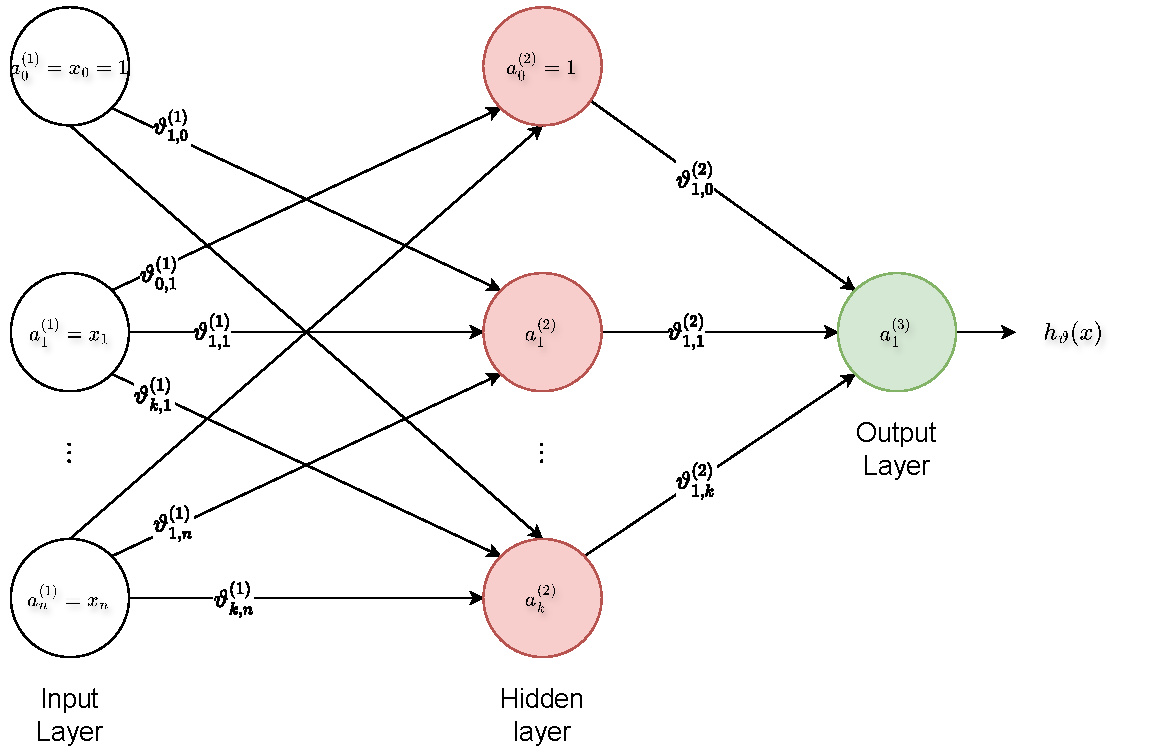
\includegraphics[width=0.75\textwidth]{images/NeuralNet1pdf.pdf}
\caption{Un Multi-Layer Perceptron con un input layer (in bianco, $a_i^{(1)} = x_i$), un hidden layer con $k$ neuroni (in rosso) e un output layer con un solo neurone (in verde) che restituisce $h_\vartheta(x)$. Le unità $a_0^{(1)}$ e $a_0^{(2)}$ sono i bias, sempre pari a 1; i pesi $\vartheta_{ji}^{(l)}$ sono riportati sugli archi.}
\label{fig:mlp}
\end{figure}

\paragraph{Notazione.}
Indichiamo con:
\begin{itemize}
    \item $a_i^{(l)}$ l'\textbf{attivazione} della $i$-esima unità del layer $l$; nell'input layer $a_i^{(1)} = x_i$.
    \item $\vartheta_{ji}^{(l)}$ il parametro che collega l'unità $i$ del layer $l$ (di partenza) all'unità $j$ del layer $l+1$ (di arrivo).
    \item $\vartheta^{(l)}$ la matrice dei parametri che mappa il layer $l$ nel layer $l+1$.
\end{itemize}

Ogni neurone calcola una combinazione lineare delle attivazioni del layer precedente e vi applica una \textbf{funzione di attivazione} $f$:
\[
z_j^{(l)} = \sum_{i} \vartheta_{ji}^{(l-1)}\, a_i^{(l-1)} = \vartheta_{j0}^{(l-1)}a_0^{(l-1)} + \vartheta_{j1}^{(l-1)}a_1^{(l-1)} + \dots, \qquad a_j^{(l)} = f\big(z_j^{(l)}\big)
\]
o, in forma matriciale, $z^{(l)} = \vartheta^{(l-1)}a^{(l-1)}$ e $a^{(l)} = f(z^{(l)})$, dove $f$ è applicata elemento per elemento. Nel caso della figura~\ref{fig:mlp}, l'output della rete è quindi:
\[
\begin{aligned}
h_\vartheta(x) = a_1^{(3)} &= f\big(\vartheta_{10}^{(2)} + \vartheta_{11}^{(2)}a_1^{(2)} + \dots + \vartheta_{1k}^{(2)}a_k^{(2)}\big) \\
&= f\Big(\vartheta_{10}^{(2)} + \vartheta_{11}^{(2)}\underbrace{f\big(\vartheta_{10}^{(1)} + \dots + \vartheta_{1n}^{(1)}a_n^{(1)}\big)}_{a_1^{(2)}} + \dots + \vartheta_{1k}^{(2)}\underbrace{f\big(\vartheta_{k0}^{(1)} + \dots + \vartheta_{kn}^{(1)}a_n^{(1)}\big)}_{a_k^{(2)}}\Big)
\end{aligned}
\]
Una rete neurale è quindi una \textbf{composizione di funzioni derivabili}.

\paragraph{Numero di parametri.}
Se la rete ha $s_l$ unità nel layer $l$ e $s_{l+1}$ unità nel layer $l+1$, la matrice $\vartheta^{(l)}$ ha dimensione $s_{l+1} \times (s_l + 1)$, dove il $+1$ tiene conto dell'unità di bias. Ad esempio, una rete con 2 feature in input, un hidden layer con 3 neuroni e un output layer con 2 neuroni ha $\vartheta^{(1)} \in \mathbb{R}^{3 \times 3}$ e $\vartheta^{(2)} \in \mathbb{R}^{2 \times 4}$, per un totale di $9 + 8 = 17$ parametri.

\subsection{Le due parti di una rete neurale}
Una rete neurale per la classificazione è composta da due parti (figura~\ref{fig:nn-parti}):
\begin{itemize}
    \item \textbf{Feature learning}: la prima parte della rete impara, in modo supervisionato e a seconda del task, come trasformare l'input $x$ in una rappresentazione utile, nell'esempio $a^{(2)}$.
    \item \textbf{Classificatore}: l'ultima parte è un softmax (o una regressione logistica, nel caso binario) che prende in input le feature apprese.
\end{itemize}

\begin{figure}[htbp]
\centering
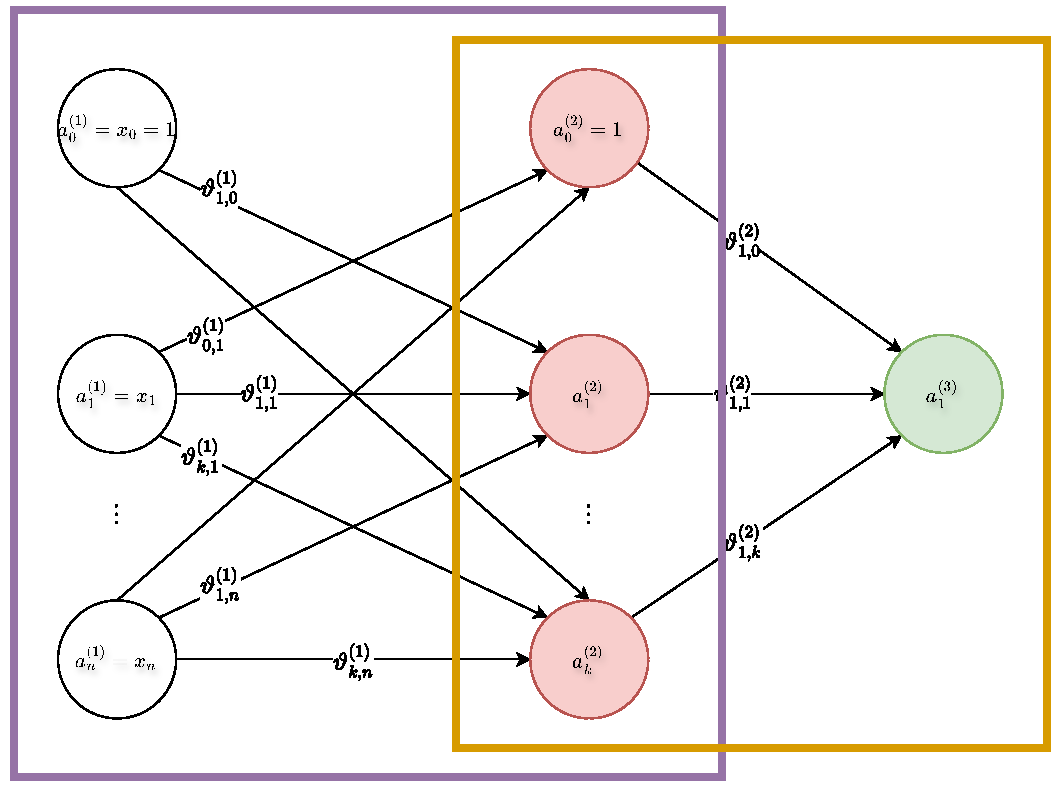
\includegraphics[width=0.7\textwidth]{images/NeuralNet2pdf.pdf}
\caption{Le due parti di una rete neurale: il riquadro viola evidenzia la trasformazione appresa dell'input $x$ nelle feature $a^{(2)}$, mentre il riquadro arancione evidenzia il classificatore (softmax o regressione logistica) che usa le feature apprese.}
\label{fig:nn-parti}
\end{figure}

Si possono aggiungere tutti gli hidden layer necessari per adattare la rete a un problema non lineare, rendendola \textbf{profonda} (\emph{deep}). Hidden layer diversi possono avere un numero diverso di neuroni. La funzione di attivazione, invece, è in genere la stessa per tutti i neuroni (si possono usare funzioni diverse, ma si tratta di casi particolari). Al crescere della dimensione dell'input aumenta la probabilità che lo spazio sia non lineare, e può quindi servire aggiungere layer, neuroni per layer, o entrambi.

\subsection{Funzioni di attivazione}
Le funzioni di attivazione \textbf{devono essere derivabili}: in questo modo la rete, essendo una composizione di funzioni derivabili, è a sua volta derivabile, e la si può addestrare con la discesa del gradiente. Le più usate sono:
\begin{center}
\renewcommand{\arraystretch}{1.6}
\begin{tabular}{@{}lll@{}}
\toprule
Nome & Funzione & Derivata \\
\midrule
Identità & $f(x) = x$ & $f'(x) = 1$ \\
Sigmoide (logistica) & $f(x) = \dfrac{1}{1 + e^{-x}}$ & $f'(x) = f(x)\big(1 - f(x)\big)$ \\
Tangente iperbolica & $f(x) = \tanh(x) = \dfrac{2}{1 + e^{-2x}} - 1$ & $f'(x) = 1 - f(x)^2$ \\
ReLU & $f(x) = \max(0, x)$ & $f'(x) = \mathbf{1}\{x \ge 0\}$ \\
Softplus & $f(x) = \log(1 + e^{x})$ & $f'(x) = \dfrac{1}{1 + e^{-x}}$ \\
\bottomrule
\end{tabular}
\end{center}

\begin{figure}[htbp]
\centering
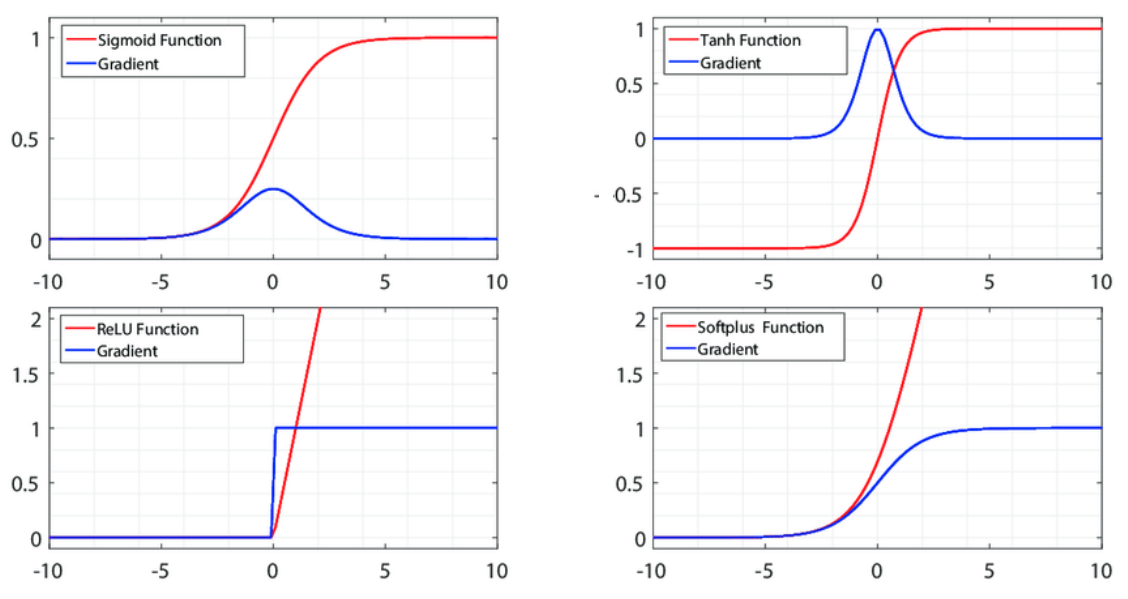
\includegraphics[width=0.8\textwidth]{images/activation-functions.png}
\caption{Le funzioni di attivazione più usate (in rosso) e le relative derivate (in blu): sigmoide (in alto a sinistra), tangente iperbolica (in alto a destra), ReLU (in basso a sinistra) e softplus (in basso a destra). Si noti come la derivata della softplus sia proprio la sigmoide.}
\label{fig:attivazioni}
\end{figure}

\subsection{Il teorema di approssimazione universale}
Il motivo per cui le reti neurali funzionano così bene su problemi non lineari è formalizzato dal seguente risultato.

\begin{teorema}[Approssimazione universale]\label{teo:uat}
Una rete neurale feedforward\footnote{Per feedforward si intende una rete in cui ogni layer riceve input esclusivamente dal layer precedente e lo trasmette al successivo, senza cicli.} con un solo hidden layer, dotata di un numero finito ma sufficientemente grande di neuroni e di una funzione di attivazione non lineare e non polinomiale (ad esempio la sigmoide), è in grado di approssimare qualunque funzione continua $f : C \to \mathbb{R}$ definita su un insieme compatto $C \subset \mathbb{R}^n$ con errore arbitrariamente piccolo, ovvero per ogni $\varepsilon > 0$ esiste una rete che implementa $\hat{f}$ tale che
\[
\sup_{x \in C}\big|f(x) - \hat{f}(x)\big| < \varepsilon.
\]
\end{teorema}

Il teorema garantisce quindi che un solo hidden layer è sufficiente a \emph{rappresentare} qualunque funzione continua, ma non dice nulla su quanto questo sia praticabile: come osservato in \cite{Goodfellow-et-al-2016}, il layer potrebbe dover essere enormemente grande e la rete potrebbe non riuscire ad apprendere e generalizzare correttamente. Il teorema non fornisce infatti né un metodo per trovare i parametri, né un limite al numero di neuroni necessari. In pratica, l'uso di più hidden layer permette spesso di rappresentare le stesse funzioni in modo più compatto: questa è una delle motivazioni delle reti \emph{deep}.

\subsection{Classificazione multiclasse e regressione}
Le reti neurali permettono di addestrare ipotesi complesse e non lineari sullo spazio delle feature, a seconda del task:
\begin{itemize}
    \item \textbf{Classificazione binaria}: basta un solo neurone di output, con $y^{(i)} \in \{0, 1\}$.
    \item \textbf{Classificazione multiclasse}: con $K \ge 3$ classi si usano $K$ unità di output e le etichette sono vettori one-hot, $y^{(i)} \in \{0, 1\}^K$, con un solo 1 nella posizione corrispondente alla classe. Come visto in figura~\ref{fig:nn-standard}, l'output layer è un softmax.
    \item \textbf{Regressione}: si eliminano logit e normalizzazione, si usa una regressione lineare nell'ultimo layer (ogni nodo di output è un regressore lineare) e si cambia la funzione di costo, usando la \textbf{MSE loss}, che deve tenere conto dell'output di tutti i regressori (figura~\ref{fig:nn-regressione}).
\end{itemize}

\begin{figure}[htbp]
\centering
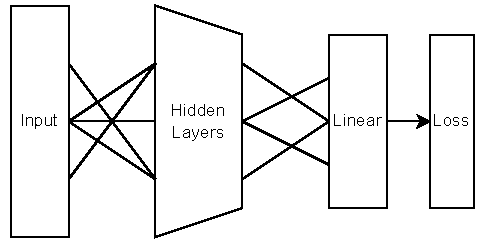
\includegraphics[width=0.6\textwidth]{images/linear-reg-neuralnet.pdf}
\caption{Struttura di una rete neurale per la regressione: dopo gli hidden layer l'ultimo blocco è un modello lineare, la cui uscita viene confrontata con il target tramite la MSE loss.}
\label{fig:nn-regressione}
\end{figure}

\section{Training e inferenza}
Supponiamo di aver definito un'architettura. Durante la fase di \textbf{training} l'obiettivo è imparare i parametri migliori per il modello, e per farlo servono una funzione di loss e un algoritmo che li apprenda. Una volta ottenuti i parametri, questi vengono usati per fare \textbf{inferenza} su nuovi pattern.

\paragraph{Funzione di costo.}
Per la classificazione vogliamo trovare $\hat{\vartheta}$ tale che
\[
\hat{\vartheta} = \arg\min_\vartheta J(\vartheta), \qquad J(\vartheta) = -\frac{1}{m}\sum_{i=1}^{m}\sum_{c=0}^{K-1}\mathbf{1}\{y^{(i)} = c\}\log h_\vartheta^{(c)}(x^{(i)})
\]
ovvero la somma delle cross-entropy di tutti i neuroni di output. Per raggiungere l'obiettivo dobbiamo essere in grado di calcolare in modo efficiente
\[
\frac{\partial J(\vartheta)}{\partial \vartheta_{ji}^{(l)}} \qquad \forall j, i, l.
\]

\paragraph{Overfitting.}
Le dimensioni della rete determinano un trade-off. Una rete ``piccola'' ha pochi parametri, è computazionalmente più economica ma è più soggetta a underfitting. Una rete ``grande'' ha molti parametri, è più soggetta a overfitting ed è computazionalmente più costosa; in questo caso si usa la regolarizzazione ($\lambda$) per contrastare l'overfitting.

\paragraph{Inizializzazione dei parametri.}
Come inizializzare la matrice dei parametri $\vartheta$? Se si assegnassero gli stessi valori ai pesi che partono dallo stesso nodo, i nodi di arrivo calcolerebbero esattamente le stesse cose e riceverebbero gli stessi gradienti, comportandosi come un unico neurone. Per questo motivo si effettua il \textbf{symmetry breaking}: i parametri che dipendono dallo stesso nodo devono essere inizializzati con valori diversi e piccoli, tipicamente scelti casualmente in un intervallo $\vartheta_{ji}^{(l)} \in [-\varepsilon, \varepsilon]$.

\section{Come si apprendono i parametri?}\label{sec:problema-learning}
Arriviamo così al problema centrale: come si apprendono i parametri di una rete neurale con un numero di hidden layer $\geq 1$? Riepilogando quanto visto finora:
\begin{itemize}
    \item \textbf{Un solo neurone}: si usa la discesa del gradiente, evoluzione dell'algoritmo di learning di Rosenblatt.
    \item \textbf{Softmax}: si usa la discesa del gradiente, perché la loss agisce su un solo layer di pesi.
    \item \textbf{Rete con hidden layer}: i valori dei nodi nascosti non sono noti in anticipo, ovvero il training set non fornisce alcuna ground truth per i layer intermedi.
\end{itemize}
Di conseguenza non possiamo più usare la discesa del gradiente nella forma classica, ma dobbiamo rivedere il modo in cui calcoliamo le derivate rispetto ai parametri. La soluzione si basa sul fatto che le reti neurali sono \textbf{grafi computazionali}, su cui si può usare la \textbf{chain rule} per spostare i gradienti all'indietro: è l'algoritmo di \textbf{backpropagation}, oggetto del prossimo capitolo.

In sintesi, il softmax risolve la classificazione multiclasse ma resta un modello lineare; le reti neurali imparano anche la rappresentazione dei dati e possono approssimare funzioni non lineari arbitrarie, al prezzo di dover calcolare i gradienti rispetto a parametri di layer di cui non conosciamo l'uscita attesa.

\section*{Riferimenti}
Il materiale visto in questo capitolo comprende:
\begin{itemize}
    \item Materiale visto a lezione (13 ottobre 2026).
    \item Slide del corso \emph{Softmax -- Generalization of Logistic Regression} e \emph{Neural Network -- Multi-Layer Perceptron \& Deep Learning}.
    \item Riassunto dei capitoli 2, 4 e 6 delle dispense di \emph{Machine Learning}, da cui sono tratte anche tutte le figure di questo capitolo: \url{https://github.com/emanuelegaliano/Machine-Learning}.
    \item Teorema di approssimazione universale dal libro \citetitle{Goodfellow-et-al-2016} \cite{Goodfellow-et-al-2016}, sezione 6.4.1.
\end{itemize}

\chapter{Backpropagation}\label{ch:backprop}
Nel capitolo precedente abbiamo visto che una rete neurale con almeno un hidden layer non può essere addestrata con la discesa del gradiente nella forma classica, perché il training set non fornisce alcuna ground truth per i layer intermedi. Eppure la discesa del gradiente ha bisogno, per ogni parametro della rete, della derivata della funzione di costo rispetto a quel parametro. La \textbf{backpropagation} è l'algoritmo che permette di calcolare tutte queste derivate in modo efficiente, sfruttando il fatto che una rete neurale è un \textbf{grafo computazionale} e che sui grafi computazionali la chain rule si applica in modo del tutto meccanico. In questo capitolo introduciamo i grafi computazionali e il modo in cui si valutano in avanti e all'indietro.

\section{Il problema dell'apprendimento}
Consideriamo una rete come quella in figura~\ref{fig:rete-esempio}, con 2 feature in input (estese con il bias), un hidden layer con 3 neuroni (più il bias) e un output layer con 2 neuroni. Indichiamo con $\vartheta$ l'insieme di tutti i parametri della rete, ovvero le matrici $\vartheta^{(1)} \in \mathbb{R}^{3\times 3}$ e $\vartheta^{(2)} \in \mathbb{R}^{2 \times 4}$.

\begin{figure}[htbp]
\centering
\begin{tikzpicture}[>=Stealth, node distance=1.1cm,
  neuron/.style={draw, circle, minimum size=8mm, inner sep=0pt, font=\scriptsize}]
  % input
  \node[neuron] (i0) at (0,1.6) {$1$};
  \node[neuron] (i1) at (0,0.4) {$x_1$};
  \node[neuron] (i2) at (0,-0.8) {$x_2$};
  % hidden
  \node[neuron, draw=red!70!black] (h0) at (3,2.2) {$1$};
  \node[neuron, draw=red!70!black] (h1) at (3,1.0) {$a_1^{(2)}$};
  \node[neuron, draw=red!70!black] (h2) at (3,-0.2) {$a_2^{(2)}$};
  \node[neuron, draw=red!70!black] (h3) at (3,-1.4) {$a_3^{(2)}$};
  % output
  \node[neuron, draw=Accent] (o1) at (6,1.0) {$a_1^{(3)}$};
  \node[neuron, draw=Accent] (o2) at (6,-0.4) {$a_2^{(3)}$};
  \foreach \i in {i0,i1,i2} \foreach \h in {h1,h2,h3} \draw[->, TextGray] (\i) -- (\h);
  \foreach \h in {h0,h1,h2,h3} \foreach \o in {o1,o2} \draw[->, TextGray] (\h) -- (\o);
  \node[font=\scriptsize, TextGray] at (1.5,-2.2) {$\vartheta^{(1)} \in \mathbb{R}^{3\times 3}$};
  \node[font=\scriptsize, TextGray] at (4.5,-2.2) {$\vartheta^{(2)} \in \mathbb{R}^{2\times 4}$};
  \draw[->] (o1) -- ++(1.1,0) node[right, font=\scriptsize] {$h_\vartheta^{(1)}(x)$};
  \draw[->] (o2) -- ++(1.1,0) node[right, font=\scriptsize] {$h_\vartheta^{(2)}(x)$};
\end{tikzpicture}
\caption{Una rete con 2 feature in input, un hidden layer con 3 neuroni (in rosso) e un output layer con 2 neuroni (in verde petrolio); i nodi con valore 1 sono le unità di bias. La matrice $\vartheta^{(1)}$ mappa l'input nell'hidden layer, la matrice $\vartheta^{(2)}$ mappa l'hidden layer nell'output.}
\label{fig:rete-esempio}
\end{figure}

\paragraph{Feedforward propagation.}
Prendendo in esempio la figura \ref{fig:rete-esempio}, abbiamo una rete già trainata con cui fare inferenza (quindi con i pesi $\vartheta$ fissati). Dato un input $x = [x_1, x_2]^T$, l'output della rete si calcola propagando in avanti le attivazioni dei neuroni. Le attivazioni del layer di input sono $a_0^{(1)} = x_0 = 1$, $a_1^{(1)} = x_1$ e $a_2^{(1)} = x_2$. Per calcolare le attivazioni dei layer successivi, si moltiplica la matrice dei pesi per il vettore delle attivazioni del layer precedente e si applica la funzione di attivazione $f$:
\[
  a_j^{(2)} = f(\sum_{i=0}^2 \vartheta_{j, i}^{(1)} a_i^{(1)}), \qquad j = 1, 2, 3
\]
dove rappresentiamo con $a_i^{(1)}$ le attivazioni del layer di input. 

Volendo generalizzare questa forma, dobbiamo considerare una rete con $L$ layer, dove il layer $l$ ha $s_l$ unità. Quindi il layer $l+1$ ha $s_{l+1}$ unità, e la matrice dei pesi $\vartheta^{(l)}$ ha dimensione $s_{l+1} \times (s_l + 1)$, dove il +1 è per il bias. Le attivazioni del layer $l+1$ si calcolano come:
\[
a_j^{(l+1)} = f\Big(\sum_{i=0}^{s_l}\vartheta_{j,i}^{(l)}a_i^{(l)}\Big), \qquad j = 1, \dots, s_{l+1},
\]
con $a_0^{(l)} = 1$ per ogni $l$ (unità di bias). In forma vettoriale, indicando con $a^{(l)} \in \mathbb{R}^{s_l+1}$ il vettore delle attivazioni del layer $l$ (bias incluso) e con $f$ applicata elemento per elemento:
\[
z^{(l+1)} = \vartheta^{(l)}a^{(l)}, \qquad a^{(l+1)} = \begin{bmatrix} 1 \\ f\big(z^{(l+1)}\big) \end{bmatrix}.
\]
Il vettore $z^{(l+1)} \in \mathbb{R}^{s_{l+1}}$ contiene le somme pesate prima dell'attivazione. Il prodotto è ben definito perché $\vartheta^{(l)}$ ha $s_l + 1$ colonne, esattamente la lunghezza di $a^{(l)}$.

La feedforward propagation consiste quindi \textbf{nel ripetere} questo passo da $l = 1$ a $l = L-1$, partendo dall'input:
\begin{enumerate}
    \item $a^{(1)} = [1, x_1, \dots, x_n]^T$, dove $n = s_1$ è il numero di feature.
    \item Per $l = 1, \dots, L-1$: calcolare $z^{(l+1)} = \vartheta^{(l)}a^{(l)}$ e $a^{(l+1)} = f\big(z^{(l+1)}\big)$, aggiungendo il bias $a_0^{(l+1)} = 1$ se $l+1 < L$.
    \item L'output della rete è $h_\vartheta(x) = a^{(L)} \in \mathbb{R}^{s_L}$.
\end{enumerate}
Nell'ultimo layer non si aggiunge il bias, perché non c'è un layer successivo a cui trasmetterlo.

\paragraph{Learning.}
Il problema dell'apprendimento consiste nel trovare l'insieme ottimale di pesi per cui la rete $h_\vartheta$ approssima il più possibile una funzione $F$, rispetto a una funzione di loss. La funzione $F$ non è data esplicitamente, ma solo implicitamente, attraverso gli esempi del training set. I pesi sono numeri reali piccoli, inizializzati casualmente e rispettando il symmetry breaking. Per determinarli bisogna usare la discesa del gradiente per ottenere il minimo della funzione di costo:
\[
J(\vartheta) = \frac{1}{2m}\sum_{i=1}^{m}L\big(\vartheta, x^{(i)}, y^{(i)}\big) + \underbrace{\frac{\lambda}{2}\sum_{l=1}^{L-1}\sum_{i=1}^{s_l}\sum_{j=1}^{s_{l+1}}\big(\vartheta_{ji}^{(l)}\big)^2}_{\text{regolarizzazione}}
\]
dove $L$ è la loss function, ovvero la cross-entropy per la classificazione o la MSE per la regressione. La discesa del gradiente richiede le derivate di $J(\vartheta)$ rispetto a ogni parametro:
\[
\vartheta_{ji}^{(l)} \leftarrow \vartheta_{ji}^{(l)} - \alpha\frac{\partial J(\vartheta)}{\partial \vartheta_{ji}^{(l)}}.
\]

Calcolare a mano la derivata per ogni cammino della rete è inefficiente, perché molti cammini condividono gli stessi tratti e gli stessi calcoli verrebbero ripetuti più volte. Serve quindi un algoritmo più furbo, che sfrutti due osservazioni:
\begin{enumerate}
    \item La rete è una composizione di funzioni derivabili.
    \item Vale la proprietà della \textbf{chain rule}: se $F(x) = f(g(x))$, allora $F'(x) = g'(x)\,f'\big(g(x)\big)$.
\end{enumerate}
Per trovare un modo efficiente di calcolare il gradiente su una rete si ricorre ai grafi computazionali.

\section{Grafi computazionali}
\begin{definizione}[Grafo computazionale]
Un \textbf{grafo computazionale} è un grafo orientato in cui:
\begin{itemize}
    \item I \textbf{nodi} sono unità di calcolo: ogni nodo calcola una singola \textbf{funzione primitiva} del proprio input, ad esempio una somma, un prodotto o $1/x$.
    \item Gli \textbf{archi} trasmettono informazione numerica da un nodo all'altro, in avanti; un arco può essere \textbf{pesato}, e quando il peso non è indicato vale 1.
\end{itemize}
Le funzioni primitive devono essere \textbf{continue} e \textbf{derivabili}.
\end{definizione}

Una rete neurale feedforward rappresenta una catena di composizioni di funzioni che trasforma un input in un output, ed è quindi un grafo computazionale: i neuroni sono i nodi, i pesi $\vartheta_{ji}^{(l)}$ sono i pesi degli archi e le funzioni di attivazione sono le primitive dei nodi, assunte uguali per tutti i nodi.

\begin{figure}[htbp]
\centering
\begin{tikzpicture}[>=Stealth]
  \node[opnode] (x) at (0,1.2) {$x$};
  \node[opnode] (y) at (0,0) {$y$};
  \node[opnode] (z) at (0,-1.4) {$z$};
  \node[opnode, draw=teal!80!black, fill=teal!18, thick] (s1) at (2,0.6) {$+$};
  \node[opnode, draw=teal!80!black, fill=teal!18, thick] (s2) at (4,-0.4) {$+$};
  \draw[flow] (x) -- node[above, fwd] {$1$} (s1);
  \draw[flow] (y) -- node[below, fwd] {$1$} (s1);
  \draw[flow] (s1) -- node[above right, fwd] {$1$} (s2);
  \draw[flow] (z) -- node[below, fwd] {$1$} (s2);
  \draw[flow] (s2) -- (5.4,-0.4) node[right] {$f(x,y,z)$};
  \node[font=\scriptsize, TextGray, above] at (2,1.0) {$x+y$};
\end{tikzpicture}
\caption{Esempio di Grafo Computazionale. Viene rappresentata la funzione $f(x,y,z) = (x+y)+z$: i nodi con lo sfondo verde petrolio calcolano la funzione primitiva somma, gli archi trasmettono i valori da sinistra verso destra e hanno tutti peso 1.}
\label{fig:grafo-somma}
\end{figure}

\paragraph{Esempio.}
Consideriamo la figura \ref{fig:grafo-somma}, che rappresenta un grafo computazionale per la funzione
\[
f(x, y, z) = (x + y) + z.
\]
La somma è una funzione primitiva, per cui la funzione si scompone in due nodi: il primo calcola $x + y$, il secondo somma $z$ al risultato del primo.

\subsection{B-diagram}
Per poter calcolare le derivate, si dà a ogni nodo della rete una struttura composta, ottenendo un \textbf{backpropagation diagram} (B-diagram). 
\begin{definizione}[B-diagram]
  Un \textbf{B-diagram} è un grafo orientato in cui ogni nodo è diviso in due metà: \begin{itemize}
    \item la parte destra calcola la funzione primitiva del nodo;
    \item la parte sinistra calcola la derivata della funzione primitiva del nodo.
  \end{itemize}
\end{definizione}

Gli archi non hanno più una freccia, perché il grafo può essere percorso sia in avanti sia all'indietro (Figura \ref{fig:bnode}).

\begin{figure}[htbp]
\centering
\begin{tikzpicture}
  \node[bnode, minimum height=12mm, font=\normalsize] (n) at (0,0) {$f'$ \nodepart{two} $f$};
  \draw (n.west) -- ++(-1.4,0);
  \draw (n.east) -- ++(1.4,0);
  \node[font=\scriptsize, anchor=east, align=right] at (-0.6,-1.2) {derivata della\\funzione primitiva};
  \node[font=\scriptsize, anchor=west, align=left] at (0.6,-1.2) {funzione primitiva\\del nodo};
  \draw[->, TextGray] (-0.8,-0.85) -- (-0.3,-0.4);
  \draw[->, TextGray] (0.8,-0.85) -- (0.3,-0.4);
\end{tikzpicture}
\hspace{1.5cm}
\begin{tikzpicture}
  \node[bnode] (s) at (0,0) {$1$ \nodepart{two} $+$};
  \node[bnode] (a) at (2.6,0) {$\sigma'$ \nodepart{two} $\sigma$};
  \draw (s.west) -- ++(-0.8,0.5);
  \draw (s.west) -- ++(-0.9,0);
  \draw (s.west) -- ++(-0.8,-0.5);
  \draw (s.east) -- (a.west);
  \draw (a.east) -- ++(0.9,0);
\end{tikzpicture}
\caption{A sinistra, un nodo di un B-diagram: la metà destra contiene la funzione primitiva $f$, la metà sinistra la sua derivata $f'$. A destra, un neurone con attivazione sigmoide scomposto in due nodi: un nodo di integrazione (somma), la cui derivata rispetto a ogni input è 1, seguito dal nodo di attivazione $\sigma$.}
\label{fig:bnode}
\end{figure}

\paragraph{Nodi di integrazione e di attivazione.}
Considerando le funzioni primitive, conviene separare la funzione di integrazione, ovvero la somma degli input di un neurone, dalla funzione di attivazione. Ad esempio, un neurone con attivazione sigmoide, il cui input è una combinazione lineare $z = \sum_i \vartheta_i x_i$, diventa la coppia di nodi a destra in figura~\ref{fig:bnode}: il nodo somma ha derivata 1 rispetto a ciascun input, mentre il nodo di attivazione calcola
\[
\sigma(z) = \frac{1}{1 + e^{-z}}, \qquad \sigma'(z) = \sigma(z)\big(1 - \sigma(z)\big) = \frac{1}{1 + e^{-z}}\left(1 - \frac{1}{1 + e^{-z}}\right).
\]
Gli archi tra un nodo e l'altro possono essere pesati.

\subsection{Valutazione in due passi}
Per il training, la rete viene valutata in due passi:
\begin{enumerate}
    \item \textbf{Feedforward step}: l'informazione va da sinistra verso destra. In ogni nodo vengono valutate sia le funzioni primitive (lato destro) sia le loro derivate (lato sinistro), e i risultati vengono memorizzati. I risultati del lato destro vengono inoltrati alle unità connesse sulla destra.
    \item \textbf{Backward step}: serve a valutare gli errori e a propagarli all'indietro per aggiornare i parametri. In questo caso vengono usati i risultati del lato sinistro, ovvero le derivate. L'input dalla destra è sempre la costante 1.
\end{enumerate}

Per capire come si combinano le informazioni nel backward step bisogna considerare tre casi: la composizione di funzioni, la somma di funzioni e gli archi pesati.

\paragraph{Caso 1: composizione di funzioni.}
Consideriamo due nodi in serie, il primo con primitiva $g$ e il secondo con primitiva $f$, che calcolano quindi $f(g(x))$ (figura~\ref{fig:caso-composizione}). Nel feedforward step il primo nodo riceve $x$, memorizza $g'(x)$ e trasmette $g(x)$; il secondo memorizza $f'(g(x))$ e restituisce $f(g(x))$. Nel backward step si immette 1 da destra: il secondo nodo moltiplica l'input per il valore memorizzato a sinistra e trasmette $1\cdot f'(g(x))$; il primo fa lo stesso e restituisce
\[
1\cdot f'\big(g(x)\big)\,g'(x)
\]
che è esattamente la derivata della piccola rete secondo la chain rule. La backpropagation fornisce quindi un modo per implementare il principio della chain rule.

\begin{figure}[htbp]
\centering
\begin{tikzpicture}
  \node[font=\small, fwd] at (-1.4,0.9) {Feedforward};
  \node (x) at (-1.4,0) {$x$};
  \node[bnode, draw=Accent] (g) at (0.6,0) {$g'(x)$ \nodepart{two} $g(x)$};
  \node[bnode, draw=Accent] (f) at (5.0,0) {$f'(g(x))$ \nodepart{two} $f(g(x))$};
  \draw (x) -- (g.west);
  \draw (g.east) -- node[above, fwd] {$g(x)$} (f.west);
  \draw (f.east) -- ++(1.2,0) node[above left, fwd] {$f(g(x))$};
  \draw[fwd, ->, thick] (-0.6,-0.7) -- (7.2,-0.7);
  % backward
  \node[font=\small, bwd] at (-1.4,-1.5) {Backward};
  \node[bnode, draw=red!70!black] (g2) at (0.6,-2.3) {$g'(x)$ \nodepart{two} $g(x)$};
  \node[bnode, draw=red!70!black] (f2) at (5.0,-2.3) {$f'(g(x))$ \nodepart{two} $f(g(x))$};
  \draw (g2.west) -- ++(-0.6,0) node[left, bwd] {$1\cdot f'(g(x))\,g'(x)$};
  \draw (g2.east) -- node[above, bwd] {$1\cdot f'(g(x))$} (f2.west);
  \draw (f2.east) -- ++(1.0,0) node[right, bwd] {$1$};
  \draw[bwd, <-, thick] (-0.6,-3.0) -- (7.2,-3.0);
\end{tikzpicture}
\caption{Caso 1, composizione di funzioni. In alto il feedforward step (in verde petrolio): ogni nodo memorizza la propria derivata a sinistra e trasmette il valore della primitiva a destra. In basso il backward step (in rosso): partendo dalla costante 1, ogni nodo moltiplica l'input proveniente da destra per la derivata memorizzata, ottenendo all'estremo sinistro la derivata $f'(g(x))\,g'(x)$ della composizione.}
\label{fig:caso-composizione}
\end{figure}

In generale, se due nodi in serie hanno memorizzato i valori $B'$ e $A'$ durante il feedforward, il valore che attraversa all'indietro il nodo $A$ è $1\cdot A'$ e il valore che esce da $B$ è $1\cdot A' \cdot B'$, ovvero la derivata. Si noti che le derivate $g'(x)$ e $f'(g(x))$ vengono calcolate nel feedforward e usate nel backward, mentre $g(x)$ e $f(g(x))$ vengono calcolate e usate nel solo feedforward.

\paragraph{Caso 2: somma di funzioni.}
Consideriamo ora un input $x$ che viene inviato a due nodi $f_1$ e $f_2$, le cui uscite vengono sommate da un nodo $+$ (figura~\ref{fig:caso-somma}). Il nodo somma $F(x_1, x_2) = x_1 + x_2$ ha due derivate parziali, $\partial F/\partial x_1 = \partial F/\partial x_2 = 1$. Nel feedforward la rete calcola $f_1(x) + f_2(x)$. Nel backward step il nodo somma riceve 1 e lo trasmette, moltiplicato per 1, su entrambi i rami; ogni ramo lo moltiplica per la propria derivata, ottenendo $1\cdot 1\cdot f_1'(x)$ e $1\cdot 1\cdot f_2'(x)$. Andando all'indietro, \textbf{i valori che arrivano allo stesso nodo da rami diversi vengono sommati}, per cui all'estremo sinistro si ottiene
\[
f_1'(x) + f_2'(x)
\]
ovvero proprio la derivata di $f_1(x) + f_2(x)$. Un nodo il cui output viene inviato a più nodi è quindi equivalente a più copie dello stesso nodo, e i gradienti delle copie si sommano.

\begin{figure}[htbp]
\centering
\begin{tikzpicture}
  \node[bnode] (f1) at (3.2,1.0) {$f_1'(x)$ \nodepart{two} $f_1(x)$};
  \node[bnode] (f2) at (3.2,-1.0) {$f_2'(x)$ \nodepart{two} $f_2(x)$};
  \node[bnode] (s) at (6.8,0) {$1$ \nodepart{two} $+$};
  \draw (0.6,0) node[left, bwd] {$f_1'(x) + f_2'(x)$} -- (1.3,0) coordinate (b);
  \draw (b) -- node[above left, bwd, pos=0.55] {$1\cdot 1\cdot f_1'(x)$} (f1.west);
  \draw (b) -- node[below left, bwd, pos=0.55] {$1\cdot 1\cdot f_2'(x)$} (f2.west);
  \draw (f1.east) -- node[above right, bwd, pos=0.45] {$1\cdot 1$} (s.north west);
  \draw (f2.east) -- node[below right, bwd, pos=0.45] {$1\cdot 1$} (s.south west);
  \draw (s.east) -- ++(2.6,0) node[pos=0.55, above, fwd] {$f_1(x) + f_2(x)$} node[pos=0.55, below, bwd] {$1$};
\end{tikzpicture}
\caption{Caso 2, somma di funzioni. Il nodo somma restituisce $f_1(x) + f_2(x)$ nel feedforward (in verde petrolio); nel backward (in rosso) la costante 1 viene distribuita su entrambi i rami, ciascuno la moltiplica per la propria derivata e, nel punto in cui i rami si separano, i due contributi vengono sommati.}
\label{fig:caso-somma}
\end{figure}

\paragraph{Caso 3: archi pesati.}
Infine, consideriamo due nodi $A$ e $B$ collegati da un arco di peso $\vartheta$ (figura~\ref{fig:caso-pesi}). Nel feedforward il nodo $A$ restituisce $A(x)$, l'arco la moltiplica per $\vartheta$ e il nodo $B$ riceve $\vartheta A(x)$, restituendo $B(\vartheta A(x))$. Nel backward step il nodo $B$ trasmette $B'(\vartheta A(x))$, l'arco lo moltiplica per $\vartheta$ e il nodo $A$ lo moltiplica per la propria derivata, restituendo
\[
\vartheta\, B'\big(\vartheta A(x)\big)\, A'(x)
\]
che è la derivata di $B(\vartheta A(x))$ rispetto a $x$. I pesi modulano quindi i valori trasmessi \textbf{in entrambe le direzioni}.

\begin{figure}[htbp]
\centering
\begin{tikzpicture}
  \node (x) at (-1.0,0) {$x$};
  \node[bnode] (a) at (0.6,0) {$A'(x)$ \nodepart{two} $A(x)$};
  \node[bnode] (b) at (5.6,0) {$B'(\vartheta A(x))$ \nodepart{two} $B(\vartheta A(x))$};
  \draw (x) -- (a.west);
  \draw (a.east) -- node[above, fwd] {$\vartheta A(x)$} node[below, bwd] {$\vartheta B'(\vartheta A(x))$} (b.west);
  \draw (b.east) -- ++(1.8,0) node[pos=0.5, above, fwd] {$B(\vartheta A(x))$} node[pos=0.55, below, bwd] {$1$};
  \node[bwd, below left] at (0.2,-0.45) {$\vartheta B'(\vartheta A(x))A'(x)$};
\end{tikzpicture}
\caption{Caso 3, archi pesati. Sopra l'arco il valore trasmesso nel feedforward (in verde petrolio), sotto l'arco quello trasmesso nel backward (in rosso): in entrambe le direzioni il valore viene moltiplicato per il peso $\vartheta$.}
\label{fig:caso-pesi}
\end{figure}

\subsection{L'algoritmo sul grafo}
Mettendo insieme i tre casi, data una rete $F$ con input $x$, la derivata $F'(x)$ si calcola come segue:
\begin{enumerate}
    \item \textbf{Forward pass}: l'input viene valutato da sinistra verso destra lungo la rete; i valori delle funzioni primitive e delle loro derivate vengono calcolati e memorizzati in ogni nodo.
    \item \textbf{Backward pass}: la costante 1 viene imposta come input destro della rete, e la rete viene percorsa da destra verso sinistra. L'informazione che arriva a un nodo viene sommata e il risultato viene moltiplicato per il valore memorizzato nella parte sinistra del nodo e per il peso dell'arco. Il risultato finale è la derivata di $F$ rispetto a $x$.
\end{enumerate}

\begin{osservazione}
Qualunque grafo computazionale, ovvero qualunque composizione di funzioni, può essere valutato con la backpropagation per calcolarne le derivate. In questo senso la backpropagation non è un algoritmo specifico per le reti neurali, ma un modo generale di applicare la chain rule.
\end{osservazione}

\paragraph{Esempio.}
Consideriamo la funzione
\[
f(x, y, z) = (x + y)\cdot z
\]
con input $x = -2$, $y = 5$, $z = -4$. Vogliamo calcolare $\dfrac{\partial f}{\partial x}$, $\dfrac{\partial f}{\partial y}$ e $\dfrac{\partial f}{\partial z}$.

\textbf{Soluzione.} Scomponiamo la funzione nelle due primitive $q = x + y$ e $f = q\cdot z$, di cui conosciamo le derivate parziali:
\[
\frac{\partial q}{\partial x} = 1, \quad \frac{\partial q}{\partial y} = 1, \qquad \frac{\partial f}{\partial q} = z, \quad \frac{\partial f}{\partial z} = q.
\]
Per la chain rule:
\[
\frac{\partial f}{\partial x} = \frac{\partial f}{\partial q}\frac{\partial q}{\partial x} = z\cdot 1, \qquad
\frac{\partial f}{\partial y} = \frac{\partial f}{\partial q}\frac{\partial q}{\partial y} = z\cdot 1, \qquad
\frac{\partial f}{\partial z} = q.
\]
Sul grafo computazionale (figura~\ref{fig:esempio-qz}) procediamo in due passi:
\begin{enumerate}
    \item \textbf{Forward pass}: il nodo somma calcola $q = -2 + 5 = 3$, il nodo prodotto calcola $f = 3\cdot(-4) = -12$.
    \item \textbf{Backward pass}: si immette 1 a destra. Il nodo prodotto trasmette verso $q$ il valore $1\cdot z = -4$ e verso $z$ il valore $1\cdot q = 3$. Il nodo somma riceve $-4$ e lo trasmette, moltiplicato per 1, sia verso $x$ sia verso $y$.
\end{enumerate}
Si ottiene quindi $\dfrac{\partial f}{\partial x} = -4$, $\dfrac{\partial f}{\partial y} = -4$ e $\dfrac{\partial f}{\partial z} = 3$.

\begin{figure}[htbp]
\centering
\begin{tikzpicture}
  \node[bnode] (q) at (2.4,0.6) {$1,1$ \nodepart{two} $+$};
  \node[bnode] (m) at (5.4,-0.2) {$z,q$ \nodepart{two} $*$};
  \node (x) at (0,1.6) {$x$};
  \node (y) at (0,-0.4) {$y$};
  \node (z) at (0,-1.6) {$z$};
  \draw (x) -- node[above, fwd, pos=0.35] {$-2$} node[below, bwd, pos=0.35] {$-4$} (q.west);
  \draw (y) -- node[above, fwd, pos=0.35] {$5$} node[below, bwd, pos=0.35] {$-4$} (q.west);
  \draw (q.east) -- node[above, fwd] {$3$} node[below, bwd] {$-4$} (m.west);
  \draw (z) -- node[above, fwd, pos=0.3] {$-4$} node[below, bwd, pos=0.3] {$3$} (m.west);
  \draw (m.east) -- ++(1.2,0) node[pos=0.5, above, fwd] {$-12$} node[pos=0.5, below, bwd] {$1$} node[right] {$f$};
\end{tikzpicture}
\caption{Forward e backward pass per $f(x,y,z) = (x+y)\cdot z$ con $x=-2$, $y=5$, $z=-4$. Sopra gli archi i valori del forward pass (in verde petrolio), sotto gli archi i valori del backward pass (in rosso), che coincidono con le derivate parziali di $f$ rispetto a ogni variabile. Nei nodi, a sinistra, sono riportate le derivate parziali della primitiva rispetto ai due input.}
\label{fig:esempio-qz}
\end{figure}

\subsection{Il comportamento delle porte}
L'esempio precedente mostra un comportamento ricorrente dei nodi, o \emph{porte}, più comuni durante il backward pass. Indicando con $A$ il gradiente che arriva da destra (figura~\ref{fig:porte}):
\begin{itemize}
    \item \textbf{Add gate}: \emph{distribuisce} il gradiente, trasmettendo $A$ invariato a tutti i propri input.
    \item \textbf{Mul gate}: \emph{scambia} il gradiente, ovvero trasmette a ciascun input $A$ moltiplicato per il valore dell'altro input: $A\cdot y$ verso $x$ e $A\cdot x$ verso $y$.
    \item \textbf{Max gate}: \emph{instrada} il gradiente, trasmettendo $A$ solo all'input che era il massimo e $0$ agli altri, perché $\dfrac{\partial \max(x,y)}{\partial x} = \mathbf{1}\{x \geq y\}$ e $\dfrac{\partial \max(x,y)}{\partial y} = \mathbf{1}\{y \geq x\}$.
\end{itemize}
Inoltre, come visto nel caso 2, quando l'output di un nodo viene inviato a più rami \textbf{i gradienti dei rami si sommano}.

\begin{figure}[htbp]
\centering
\begin{tikzpicture}
  \foreach \cx/\op/\out/\ga/\gb/\lab in {0/+/x+y/A/A/Add gate, 4/*/x\cdot y/A\cdot y/A\cdot x/Mul gate, 8/\max/\max(x\text{,}y)/A/0/{Max gate ($x>y$)}} {
    \node[opnode, minimum size=9mm] (g) at (\cx,0) {$\op$};
    \draw (\cx-1.3,0.8) node[left, font=\small] {$x$} -- (g);
    \draw (\cx-1.3,-0.8) node[left, font=\small] {$y$} -- (g);
    \draw (g) -- (\cx+1.5,0);
    \node[fwd, above] at (\cx+1.0,0.05) {$\out$};
    \node[bwd, below] at (\cx+1.0,-0.05) {$A$};
    \node[bwd] at (\cx-0.45,0.75) {$\ga$};
    \node[bwd] at (\cx-0.45,-0.75) {$\gb$};
    \node[font=\small\bfseries] at (\cx,-1.4) {\lab};
  }
\end{tikzpicture}
\caption{Comportamento delle porte durante il backward pass, con in verde petrolio l'output del forward pass e in rosso i gradienti: la add gate distribuisce il gradiente $A$, la mul gate lo scambia moltiplicandolo per l'altro input e la max gate lo instrada verso l'input massimo.}
\label{fig:porte}
\end{figure}

\section*{Riferimenti}
Il materiale visto in questo capitolo comprende:
\begin{itemize}
    \item Materiale visto a lezione (13 ottobre 2026).
    \item Slide del corso \emph{Backpropagation (via Computational Graphs)}.
    \item Capitolo 7, \emph{The Backpropagation Algorithm}, del libro \citetitle{Rojas1996} \cite{Rojas1996}.
\end{itemize}

\chapter{Convolutional Neural Network}\label{ch:cnn}
Le \textbf{Convolutional Neural Network} (CNN) sono reti neurali pensate per elaborare immagini e, più in generale, dati organizzati su una griglia. In questo capitolo partiamo dai limiti di un MLP quando l'input è un'immagine, introduciamo l'operazione di convoluzione e vediamo come i suoi parametri (padding, stride e dilation) determinano la forma dell'output. Infine vediamo gli altri layer che compongono una CNN (attivazioni, normalizzazione, pooling e fully connected) e alcune regole pratiche per progettarla.

\section{Dalle reti neurali alle immagini}
\subsection{Representation learning}
Riprendiamo un MLP con un solo hidden layer, ad esempio con 4 input e 3 output. Rispetto al capitolo~\ref{ch:ripasso}, qui scriviamo il bias $b$ separato dai pesi $\vartheta$, come nelle slide del corso. La rete calcola:
\[
F_\vartheta(x) = \vartheta_2\, f(\vartheta_1 x + b_1) + b_2
\]
ed esegue quindi due trasformazioni:
\begin{enumerate}
    \item trasforma l'input $x$ in $a(x) = f(\vartheta_1 x + b_1)$.
    \item trasforma il risultato intermedio $a(x)$ nell'output $h(x) = \vartheta_2\, a(x) + b_2$.
\end{enumerate}
Il risultato intermedio $a(x)$ è una \textbf{rappresentazione} di $x$, e non è scelto da noi ma appreso: l'MLP sta facendo \textbf{representation learning}\footnote{Il termine \textit{representation learning} si riferisce alla capacità di una rete neurale di apprendere automaticamente rappresentazioni utili dei dati di input.}.

In generale, una rete neurale implementa una funzione che mappa l'input $x$ nell'output $y$, dati i parametri $\vartheta$:
\[
y = h(x; \vartheta) = F_\vartheta(x).
\]
Se abbiamo un numero sufficiente di coppie $\langle x^{(i)}, y^{(i)}\rangle$ (il dataset), possiamo cercare i parametri $\vartheta$ ottimali, ovvero quelli per cui
\[
\sum_i \mathrm{loss}\big(y^{(i)}, h(x^{(i)}; \vartheta)\big)
\]
è minima, dove la funzione di loss misura l'errore commesso da $h$ nel predire $y$. La ricerca dei parametri ottimali è la procedura di \textbf{training}, e l'algoritmo più usato è la backpropagation vista nel capitolo~\ref{ch:backprop}: poiché $h$ è derivabile rispetto a $\vartheta$, funziona secondo il principio della discesa del gradiente.

\paragraph{Esempio: regressione.}
Vogliamo predire il consumo di un'automobile, in miglia per gallone (mpg), a partire da tre feature: il numero di cilindri $c$, la potenza $p$ e il peso $w$. È ragionevole pensare che esista una funzione $h$ tale che
\[
\mathrm{mpg} = h(c, p, w).
\]
Come la definiamo matematicamente? Non lo facciamo: la impariamo dai dati. Il dataset \emph{Auto MPG} contiene 398 auto, e possiamo usarlo per apprendere i pesi della rete a sinistra in figura~\ref{fig:reg-class}. Trattandosi di regressione, come funzione di loss si usa la MSE.

\paragraph{Esempio: classificazione.}
Il dataset \emph{Iris} contiene 150 fiori, descritti da 4 misure e divisi in 3 specie. Vogliamo classificare un fiore a partire dalle sue misure: gli input sono quindi 4, ma quanti sono gli output? Una tecnica comune è far calcolare alla rete \textbf{un punteggio per classe} e scegliere la classe con il punteggio più alto, per cui gli output sono 3 (figura~\ref{fig:reg-class}, a destra).

In fase di training cerchiamo i pesi che assegnano un punteggio alto alla classe corretta e basso a tutte le altre. In fase di test, invece, facciamo passare il campione nella rete e scegliamo la classe con il punteggio massimo. Come loss si usa la cross-entropy, dopo aver trasformato i punteggi in probabilità con il softmax.

\begin{figure}[htbp]
\centering
\begin{tikzpicture}[>=Stealth, font=\scriptsize,
  neuron/.style={draw, circle, minimum size=5mm, inner sep=0pt},
  hid/.style={neuron, draw=Accent, fill=Accent!25}]
  % regressione
  \foreach \k/\lab in {1/cilindri, 2/potenza, 3/peso} {
    \node[neuron] (r\k) at (0,1.2-0.8*\k+0.4) {};
    \node[left] at (r\k.west) {\lab};
  }
  \foreach \k in {1,...,4} \node[hid] (rh\k) at (1.5,1.6-0.8*\k+0.4) {};
  \node[neuron] (ro) at (3,0) {};
  \node[right] at (ro.east) {mpg};
  \foreach \i in {1,2,3} \foreach \h in {1,...,4} \draw[TextGray] (r\i) -- (rh\h);
  \foreach \h in {1,...,4} \draw[TextGray] (rh\h) -- (ro);
  \node[Accent] at (1.5,1.75) {rappresentazione appresa};
  % classificazione
  \begin{scope}[xshift=7cm]
    \foreach \k in {1,...,4} \node[neuron] (c\k) at (0,1.6-0.8*\k+0.4) {};
    \draw[decorate, decoration={brace, amplitude=4pt, mirror}] (-0.35,1.3) -- (-0.35,-1.3) node[midway, left=4pt, align=right] {4 misure};
    \foreach \k in {1,...,5} \node[hid] (ch\k) at (1.5,2.0-0.8*\k+0.4) {};
    \foreach \k in {1,2,3} \node[neuron] (co\k) at (3,1.2-0.8*\k+0.4) {};
    \draw[decorate, decoration={brace, amplitude=4pt}] (3.35,1.0) -- (3.35,-1.0) node[midway, right=4pt, align=left] {3 classi};
    \foreach \i in {1,...,4} \foreach \h in {1,...,5} \draw[TextGray] (c\i) -- (ch\h);
    \foreach \h in {1,...,5} \foreach \o in {1,2,3} \draw[TextGray] (ch\h) -- (co\o);
    \node[Accent] at (1.5,2.15) {rappresentazione appresa};
  \end{scope}
\end{tikzpicture}
\caption{Due reti con un hidden layer. A sinistra, la regressione del consumo (mpg) a partire da cilindri, potenza e peso. A destra, la classificazione dei fiori del dataset Iris a partire da 4 misure, con un punteggio per ciascuna delle 3 classi. In entrambi i casi l'hidden layer (in verde petrolio) contiene la rappresentazione appresa dell'input.}
\label{fig:reg-class}
\end{figure}

\paragraph{Da shallow a deep.}
Possiamo aggiungere tutti gli hidden layer che vogliamo. Con due hidden layer, ad esempio, la rete diventa:
\[
h(x, \vartheta) = \vartheta_h\, f_2\big(\vartheta_{f_2} f_1(\vartheta_{f_1}x + b_{f_1}) + b_{f_2}\big) + b_h
\]
dove $f_1$ e $f_2$ sono le funzioni di attivazione dei due layer. Ogni layer costruisce la propria rappresentazione a partire da quella del layer precedente, per cui la rete impara delle \textbf{rappresentazioni gerarchiche}.

Serve davvero andare in profondità? In teoria no: il teorema di approssimazione universale (teorema~\ref{teo:uat}) dice che un solo hidden layer, con un numero finito di neuroni, basta ad approssimare qualunque funzione continua su un compatto di $\mathbb{R}^n$. In pratica, però, il numero di neuroni necessari può diventare enorme, ed è più utile ``scomporre'' la rete introducendo altri hidden layer.

\subsection{MLP e immagini}
Gli MLP non sono molto adatti a elaborare immagini, per tre motivi:
\begin{itemize}
    \item \textbf{Le immagini sono grandi}: anche una piccola immagine in scala di grigi di $100 \times 100$ pixel contiene 10000 valori.
    \item \textbf{Le immagini sono complesse}, e per elaborarle possono servire molti layer.
    \item Quando il numero di layer e il numero di input crescono, \textbf{il numero di parametri cresce di conseguenza}.
\end{itemize}
L'idea è quindi di ridurre il numero di parametri in ogni layer, così da poter costruire modelli più profondi.

Forniamo il seguente esempio, su cui torneremo più volte nel capitolo: il dataset \textbf{MNIST} (figura~\ref{fig:mnist}) contiene 70000 immagini di cifre scritte a mano, di $28 \times 28$ pixel, divise in 10 classi (le cifre da 0 a 9). Vogliamo classificare ogni immagine nella cifra corretta.

\begin{figure}[htbp]
\centering
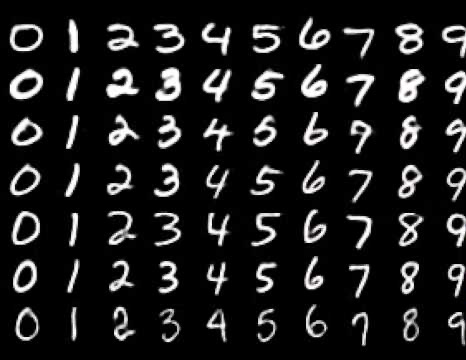
\includegraphics[width=0.5\textwidth]{images/mnist.png}
\caption{Alcune immagini del dataset MNIST: cifre scritte a mano da 0 a 9, in scala di grigi, di $28 \times 28$ pixel ciascuna.}
\label{fig:mnist}
\end{figure}

L'approccio più semplice è usare un MLP. L'immagine viene ``srotolata'' da una matrice $28 \times 28$ a un vettore $784 \times 1$, che diventa l'input di una rete con un hidden layer da 500 neuroni e un output layer da 10 neuroni, uno per classe (figura~\ref{fig:mlp-mnist}). La rete calcola:
\[
h(x, \vartheta) = \vartheta_h\, f(\vartheta_f x + b_f) + b_h
\]
dove $\vartheta_f \in \mathbb{R}^{500 \times 784}$, $b_f \in \mathbb{R}^{500}$, $\vartheta_h \in \mathbb{R}^{10 \times 500}$ e $b_h \in \mathbb{R}^{10}$. Quanti parametri ha? Basta sommare le dimensioni:
\[
500 \cdot 784 + 500 + 10 \cdot 500 + 10 = 397\,510.
\]

Un MLP così costruito funziona, ma quasi 400 mila parametri per immagini di $28 \times 28$ pixel sono tanti. Inoltre la rete tratta ogni pixel come una feature indipendente: la struttura spaziale dell'immagine va persa quando la srotoliamo.

\begin{figure}[htbp]
\centering
\begin{tikzpicture}[>=Stealth, font=\scriptsize,
  layer/.style={draw=Accent, fill=Accent!70, text=white, minimum width=6mm}]
  \node (img) at (0,0) {
\includegraphics[width=8mm]{images/mnist-4.png}};
  \node[layer, minimum height=3.2cm] (l1) at (1.5,0) {\rotatebox{90}{784}};
  \node[layer, minimum height=2.0cm] (l2) at (3.6,0) {\rotatebox{90}{500}};
  \node[layer, minimum height=1.0cm] (l3) at (5.7,0) {\rotatebox{90}{10}};
  \draw[->] (img) -- (l1);
  \draw[->] (l1) -- node[above] {$\vartheta_f, b_f$} (l2);
  \draw[->] (l2) -- node[above] {$\vartheta_h, b_h$} (l3);
  \node[TextGray] at (1.5,-1.9) {input};
  \node[TextGray] at (3.6,-1.9) {hidden layer};
  \node[TextGray] at (5.7,-1.9) {output};
\end{tikzpicture}
\caption{Un MLP per MNIST: l'immagine $28 \times 28$ viene srotolata in un vettore di 784 valori, seguito da un hidden layer con 500 neuroni e da un output layer con 10 neuroni, uno per cifra.}
\label{fig:mlp-mnist}
\end{figure}

\section{Convolutional Neural Network}
Le Convolutional Neural Network sono progettate per far scalare le reti neurali a immagini molto grandi e a sequenze video. L'idea principale è \textbf{sostituire la moltiplicazione matriciale con la convoluzione} (figura~\ref{fig:cnn-pipeline}).

\begin{figure}[htbp]
\centering
\begin{tikzpicture}[>=Stealth, font=\scriptsize,
  blk/.style={draw=Accent, fill=Accent!70, text=white, minimum width=2.1cm, minimum height=0.9cm}]
  \node[blk, draw=LemmaColor, fill=LemmaColor!70] (in) at (0,0) {Input Image};
  \node[blk] (c1) at (2.9,0) {Convolution};
  \node[blk] (c2) at (5.8,0) {Convolution};
  \node (dots) at (7.9,0) {$\cdots$};
  \draw[->] (in) -- (c1);
  \draw[->] (c1) -- (c2);
  \draw[->] (c2) -- (dots);
\end{tikzpicture}
\caption{L'idea alla base di una CNN: l'immagine in input attraversa una sequenza di convoluzioni, che prendono il posto delle moltiplicazioni matriciali di un MLP.}
\label{fig:cnn-pipeline}
\end{figure}

\begin{osservazione}[Invarianza alla traslazione]
L'estrazione delle feature dovrebbe essere \textbf{invariante alla traslazione} lungo gli assi $x$ e $y$. Pensiamo all'esempio di MNIST: un 7 resta un 7 sia che si trovi al centro dell'immagine, sia che sia spostato di qualche pixel. Una moltiplicazione matriciale imparerebbe pesi diversi in posizioni diverse, mentre la convoluzione, come vedremo, applica gli stessi pesi in tutte le posizioni e mantiene questa invarianza.
\end{osservazione}

In altre parole, una CNN impara un certo numero di \textbf{filtri}, e li impara in modo che siano i migliori per risolvere il problema dato.

\subsection{Architettura e componenti}
Una CNN è una sequenza di layer, ognuno con i propri pesi $W_l$: prima alcuni layer convoluzionali, poi alcuni layer fully connected, che restituiscono la classe (figura~\ref{fig:cnn-arch}).

\begin{figure}[htbp]
\centering
\begin{tikzpicture}[>=Stealth, font=\scriptsize,
  conv/.style={draw, minimum width=5mm, minimum height=1.5cm, inner sep=1pt},
  fc/.style={draw, minimum width=7mm, minimum height=1.5cm, inner sep=1pt}]
  \node[draw, fill=TextGray!15, minimum width=1.1cm, minimum height=1.1cm, align=center] (in) at (0,0) {immagine};
  \foreach \k in {1,...,5} \node[conv] (C\k) at (0.4+1.0*\k,0) {$C_\k$};
  \foreach \k in {6,7,8} \node[fc] (F\k) at (0.6+1.05*\k,0) {$f_\k$};
  \node[draw=ObsColor, fill=ObsColor!15, rounded corners=4pt, minimum height=6mm] (out) at (10.8,0) {bike};
  \draw[->] (in) -- (C1);
  \foreach \a/\b in {C1/C2, C2/C3, C3/C4, C4/C5, C5/F6, F6/F7, F7/F8, F8/out} \draw[->] (\a) -- (\b);
  \foreach \k in {1,...,5} \draw[<-] (C\k.south) -- ++(0,-0.6) node[below] {$W_\k$};
  \foreach \k in {6,7,8} \draw[<-] (F\k.south) -- ++(0,-0.6) node[below] {$W_\k$};
\end{tikzpicture}
\caption{Architettura di una CNN (da \cite{Krizhevsky2012}): cinque layer convoluzionali $C_1, \dots, C_5$ e tre layer fully connected $f_6, f_7, f_8$, ciascuno con i propri pesi $W_l$. L'output è la classe dell'immagine in input, nell'esempio una bicicletta.}
\label{fig:cnn-arch}
\end{figure}

I layer convoluzionali sono costruiti combinando alcuni blocchi elementari (figura~\ref{fig:cnn-blocchi}):
\begin{itemize}
    \item \textbf{Filtri lineari 3D}: $y = F * x + b$, dove $F$ è un banco di filtri e $b$ il bias. È la convoluzione vera e propria, oggetto di questo capitolo.
    \item \textbf{ReLU}: $y = \max\{0, x\}$, la non linearità applicata dopo la convoluzione.
    \item \textbf{Downsampling}: riduce la dimensione spaziale dell'input.
    \item \textbf{Normalizzazione}: normalizza le risposte su gruppi di canali con una finestra scorrevole (sliding $\ell^2$).
    \item \textbf{Spatial pooling}: $y_{ijk} = \max_{pq \in \Omega_{ij}} x_{pqk}$, ovvero per ogni canale $k$ si prende il massimo in un intorno $\Omega_{ij}$ della posizione $(i, j)$.
\end{itemize}
Gli ultimi quattro blocchi li vedremo nella sezione~\ref{sec:cnn-layer}.

\begin{figure}[htbp]
\centering
\begin{tikzpicture}[>=Stealth, font=\scriptsize,
  box/.style={draw, minimum width=1.3cm, minimum height=0.8cm, align=center}]
  \foreach \nm/\xx/\yy/\content/\formula in {
      lin/0/0/{$(F, b)$}/{$y = F * x + b$},
      down/6.6/0/{$\downarrow$}/{$y$},
      relu/0/-1.5/{}/{$y = \max\{0, x\}$},
      norm/6.6/-1.5/{sliding $\ell^2$}/{$y$},
      pool/0/-3/{$\max$}/{$y_{ijk} = \max_{pq \in \Omega_{ij}} x_{pqk}$}} {
    \node[box] (\nm) at (\xx,\yy) {\content};
    \draw[->] ([xshift=-0.7cm]\nm.west) node[left] {$x$} -- (\nm.west);
    \draw[->] (\nm.east) -- ++(0.7,0) node[right] {\formula};
  }
  \draw[->, TextGray] ([xshift=-0.45cm, yshift=-0.2cm]relu.center) -- ([xshift=0.5cm, yshift=-0.2cm]relu.center);
  \draw[->, TextGray] ([yshift=-0.35cm]relu.center) -- ([yshift=0.35cm]relu.center);
  \draw[very thick, Accent] ([xshift=-0.4cm, yshift=-0.2cm]relu.center) -- ([yshift=-0.2cm]relu.center) -- ([xshift=0.4cm, yshift=0.25cm]relu.center);
  \foreach \nm/\lab in {lin/filtri lineari 3D, down/downsampling, relu/ReLU, norm/normalizzazione, pool/spatial pooling}
    \node[TextGray, above] at (\nm.north) {\lab};
\end{tikzpicture}
\caption{I blocchi elementari dei layer convoluzionali: filtri lineari 3D, downsampling, ReLU, normalizzazione e spatial pooling. Ciascun blocco riceve un input $x$ e restituisce un output $y$.}
\label{fig:cnn-blocchi}
\end{figure}

\subsection{La convoluzione 2D}
Partiamo da un esempio (figura~\ref{fig:cane}). Applichiamo a un'immagine in scala di grigi il kernel $[1, -1]$: ogni pixel dell'output è la differenza tra un pixel dell'input e il suo vicino a destra. Nelle zone uniformi la differenza è circa 0, e infatti l'output è grigio. Dove l'intensità cambia bruscamente in orizzontale, invece, la differenza è grande: l'output mette in evidenza i \textbf{bordi verticali} dell'immagine. Un kernel, quindi, risponde a una particolare caratteristica dell'input.

\begin{figure}[htbp]
\centering
\begin{tikzpicture}[>=Stealth, font=\small]
  \node (in) at (0,0) {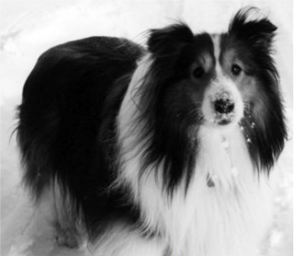
\includegraphics[width=4cm]{images/cnn-dog-input.png}};
  \node[below=0pt of in] {Input};
  \node (out) at (7.2,-1.1) {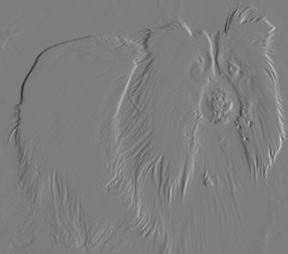
\includegraphics[width=4cm]{images/cnn-dog-output.png}};
  \node[below=0pt of out] {Output};
  \node[draw=Accent, minimum size=7mm] (k1) at (-0.35,-3.2) {$1$};
  \node[draw=Accent, minimum size=7mm, right=0pt of k1] (k2) {$-1$};
  \node[below=2pt of k1.south east] {Kernel};
  \draw[->, thick] (in.east) -- (out.west);
  \draw[->, thick] (k2.east) -- (out.west);
\end{tikzpicture}
\caption{Esempio di convoluzione 2D (da \cite{Goodfellow-et-al-2016}): il kernel $[1, -1]$ sottrae a ogni pixel il suo vicino a destra. Le zone uniformi diventano grigie, mentre i bordi verticali del cane vengono messi in evidenza.}
\label{fig:cane}
\end{figure}

In un layer possiamo imparare \textbf{più di un kernel}, in modo simile a quanto accade quando mettiamo più percettroni nello stesso layer di un MLP. Ogni kernel produce la propria uscita, e i layer successivi ricevono le uscite di tutti i kernel del layer precedente (figura~\ref{fig:multi-kernel}).

\begin{figure}[htbp]
\centering
\begin{tikzpicture}[>=Stealth, font=\scriptsize,
  blk/.style={draw=Accent, fill=Accent!70, text=white, minimum width=2.1cm, minimum height=0.9cm}]
  \node[blk, draw=LemmaColor, fill=LemmaColor!70] (in) at (0,0) {Input Image};
  \node[blk] (a1) at (3.2,0.75) {Convolution};
  \node[blk] (a2) at (3.2,-0.75) {Convolution};
  \node[blk] (b1) at (6.4,0.75) {Convolution};
  \node[blk] (b2) at (6.4,-0.75) {Convolution};
  \node (dots) at (8.6,0) {$\cdots$};
  \foreach \a in {a1,a2} \draw[->] (in.east) -- (\a.west);
  \foreach \a in {a1,a2} \foreach \b in {b1,b2} \draw[->] (\a.east) -- (\b.west);
\end{tikzpicture}
\caption{Più kernel per layer: ogni layer impara due convoluzioni, e ognuna di quelle del secondo layer riceve le uscite di entrambe quelle del primo.}
\label{fig:multi-kernel}
\end{figure}

\paragraph{Cross-correlation.}
I pesi da apprendere in un layer convoluzionale sono \textbf{i valori del kernel}. Consideriamo la figura~\ref{fig:cross-corr}: l'input è una matrice $3 \times 4$ e il kernel una matrice $2 \times 2$. Il kernel scorre sull'input e, in ogni posizione, moltiplica elemento per elemento i valori sovrapposti e li somma. Ad esempio, nella prima posizione l'output vale $aw + bx + ey + fz$. Il kernel ha solo 4 pesi, e questi restano 4 qualunque sia la dimensione dell'input.

\begin{figure}[htbp]
\centering
\begin{tikzpicture}[>=Stealth, font=\scriptsize]
  % input
  \node[TextGray] at (1.2,0.3) {Input};
  \numgrid[draw=Accent]{(0,0)}{0.6}{{a,b,c,d},{e,f,g,h},{i,j,k,l}}
  \cellrect[very thick, red!70!black]{(0,0)}{0.6}{0}{0}{2}{2}
  % kernel
  \node[TextGray] at (3.9,0.3) {Kernel};
  \numgrid[draw=Accent]{(3.3,0)}{0.6}{{w,x},{y,z}}
  % output
  \node[TextGray, anchor=east] at (0.1,-3.6) {Output};
  \foreach \rr/\cc/\sopra/\sotto in {0/0/aw + bx/ey + fz, 0/1/bw + cx/fy + gz, 0/2/cw + dx/gy + hz,
                                     1/0/ew + fx/iy + jz, 1/1/fw + gx/jy + kz, 1/2/gw + hx/ky + lz}
    \node[draw=Accent, minimum width=1.6cm, minimum height=0.9cm, align=center, anchor=north west]
      (o\rr\cc) at (0.2+1.75*\cc,-2.6-1.05*\rr) {$\sopra\, +$ \\ $\sotto$};
  \draw[very thick, red!70!black] (o00.north west) rectangle (o00.south east);
  \draw[->, red!70!black] (0.6,-1.2) -- (o00.north);
  \draw[->, red!70!black] (3.9,-1.2) to[out=-90, in=30] (o00.north east);
\end{tikzpicture}
\caption{Cross-correlation 2D (da \cite{Goodfellow-et-al-2016}): un kernel $2 \times 2$ scorre su un input $3 \times 4$ e produce un output $2 \times 3$. In rosso la prima posizione del kernel e il valore corrispondente dell'output. I pesi da apprendere sono soltanto i 4 valori del kernel.}
\label{fig:cross-corr}
\end{figure}

Formalizziamo. Sia $F$ l'immagine in input e $h$ un kernel di dimensione $(2k+1) \times (2k+1)$, con indici che vanno da $-k$ a $k$. La \textbf{cross-correlation} si definisce come:
\[
G = h \otimes F, \qquad G[i, j] = \sum_{u=-k}^{k}\sum_{v=-k}^{k} h[u, v]\, F[i + u, j + v]
\]
mentre la \textbf{convoluzione} si definisce come:
\[
G = h * F, \qquad G[i, j] = \sum_{u=-k}^{k}\sum_{v=-k}^{k} h[u, v]\, F[i - u, j - v]
\]
dove $G$ è l'output. L'unica differenza è il segno degli indici: la convoluzione equivale a una cross-correlation con il kernel \textbf{ribaltato} su entrambi gli assi, ovvero ruotato di $180^\circ$ (figura~\ref{fig:flip}).

\begin{figure}[htbp]
\centering
\begin{tikzpicture}[font=\small]
  \foreach \xx/\lab/\vals in {0/{Kernel $F$}/{{a,b,c},{d,e,f},{g,h,i}}, 4.2/{Kernel ribaltato}/{{i,h,g},{f,e,d},{c,b,a}}} {
    \numgrid[draw=Accent, font=\small]{(\xx,0)}{0.6}{\vals}
    \foreach \lb [count=\cc from 0] in {-1,0,1} {
      \node[font=\scriptsize, TextGray] at (\xx+0.3+0.6*\cc,0.25) {$\lb$};
      \node[font=\scriptsize, TextGray] at (\xx-0.3,-0.3-0.6*\cc) {$\lb$};
    }
    \node at (\xx+0.9,-2.15) {\lab};
  }
  \draw[->, thick, Accent] (2.1,-0.9) -- (3.7,-0.9) node[midway, above, font=\scriptsize] {$180^\circ$};
\end{tikzpicture}
\caption{A sinistra un kernel $3 \times 3$ con indici da $-1$ a $1$, a destra lo stesso kernel ribaltato su entrambi gli assi. Calcolare la convoluzione con il kernel di sinistra equivale a calcolare la cross-correlation con quello di destra.}
\label{fig:flip}
\end{figure}

\begin{osservazione}
Quella che nelle CNN chiamiamo convoluzione è in realtà, quasi sempre, una cross-correlation, come in figura~\ref{fig:cross-corr}. Nella pratica la differenza non conta: i valori del kernel vengono appresi, per cui una rete che usa la convoluzione imparerebbe semplicemente il kernel ribaltato.
\end{osservazione}

\paragraph{Esempio.}
Consideriamo l'immagine $5 \times 5$ in scala di grigi della figura~\ref{fig:sharpen}, divisa in una zona chiara (valore 2) e una scura (valore 8). Le applichiamo il kernel di \emph{sharpening}:
\[
K = \begin{bmatrix} 0 & -1 & 0 \\ -1 & 5 & -1 \\ 0 & -1 & 0 \end{bmatrix}.
\]
Calcoliamo l'output della cross-correlation, facendo scorrere il kernel solo nelle posizioni in cui sta tutto dentro l'immagine.

\textbf{Soluzione.} Le posizioni possibili sono $3 \times 3$, quindi l'output è una matrice $3 \times 3$. Nella prima posizione il kernel copre una zona uniforme, tutta di valore 2, e restituisce $5 \cdot 2 - 4 \cdot 2 = 2$: le zone uniformi restano invariate. Nella seconda posizione (in rosso in figura) il pixel centrale vale 2, mentre il suo vicino a destra vale 8:
\[
G[0, 1] = 5 \cdot 2 - (2 + 2 + 8 + 2) = -4.
\]

Spostandoci di un'altra posizione il centro vale 8 e il vicino a sinistra 2, per cui $G[0, 2] = 5 \cdot 8 - (8 + 2 + 8 + 8) = 14$. Il salto tra le due zone, che nell'input era da 2 a 8, nell'output diventa da $-4$ a 14: il kernel accentua i bordi, ed è proprio questo che rende l'immagine più nitida.

\begin{figure}[htbp]
\centering
\begin{tikzpicture}[font=\scriptsize]
  \def\csz{0.5}
  % input con sfondo proporzionale al valore
  \foreach \row [count=\ri from 0] in {{2,2,2,8,8},{2,2,2,8,8},{2,2,2,8,8},{2,2,8,8,8},{2,2,8,8,8}} {
    \foreach \v [count=\ci from 0] in \row {
      \pgfmathtruncatemacro\sh{8*\v}
      \pgfmathtruncatemacro\tv{100*(\v<6)}
      \node[draw=TextGray, minimum size=\csz cm, inner sep=0pt, anchor=north west, fill=black!\sh, text=black!\tv]
        at ({\ci*\csz},{-\ri*\csz}) {$\v$};
    }
  }
  \cellrect[very thick, red!70!black]{(0,0)}{\csz}{1}{0}{3}{3}
  \node at (1.25,0.3) {Input};
  \node[font=\large] at (2.95,-1.25) {$\otimes$};
  \numgrid[draw=Accent, minimum size=0.5cm]{(3.4,-0.5)}{\csz}{{0,-1,0},{-1,5,-1},{0,-1,0}}
  \node at (4.15,-0.2) {Kernel};
  \node[font=\large] at (5.35,-1.25) {$=$};
  % output, con sfondo proporzionale al valore (limitato tra 0 e 10)
  \foreach \row [count=\ri from 0] in {{2,-4,14},{2,-10,14},{-4,20,8}} {
    \foreach \v [count=\ci from 0] in \row {
      \pgfmathtruncatemacro\sh{8*min(max(\v,0),10)}
      \pgfmathtruncatemacro\tv{100*(\v<6)}
      \node[draw=TextGray, minimum size=\csz cm, inner sep=0pt, anchor=north west, fill=black!\sh, text=black!\tv, font=\tiny]
        at ({5.8+\ci*\csz},{-0.5-\ri*\csz}) {$\v$};
    }
  }
  \cellrect[very thick, red!70!black]{(5.8,-0.5)}{\csz}{1}{0}{1}{1}
  \node at (6.55,-0.2) {Output};
\end{tikzpicture}
\caption{Il kernel di sharpening applicato a un'immagine $5 \times 5$. Il colore delle celle segue il valore (i valori negativi sono resi in bianco, come se fossero 0). In rosso la seconda posizione del kernel e il valore corrispondente dell'output, $-4$: lungo il bordo tra le due zone il contrasto aumenta.}
\label{fig:sharpen}
\end{figure}

\subsection{Convoluzione 3D, padding, dilation e stride}
La forma dell'output di un layer convoluzionale dipende dalla forma del suo input e da alcune scelte: la forma del kernel, lo \textbf{zero padding}, la \textbf{dilation} e lo \textbf{stride}. In ogni caso valgono tre cose:
\begin{itemize}
    \item i pesi del layer corrispondono ai valori del kernel.
    \item i pesi sono \textbf{condivisi} all'interno di un canale (depth slice), ovvero lo stesso kernel viene usato in tutte le posizioni.
    \item stiamo di fatto imparando dei filtri che rispondono a parti, entità o indizi visivi dell'immagine.
\end{itemize}

\paragraph{Convoluzione 3D.}
Un'immagine a colori non è una matrice ma un \textbf{volume}: ad esempio un'immagine RGB ha 3 canali, per cui ha dimensione $W \times H \times 3$. In questo caso il kernel ha la stessa profondità dell'input: con un input di $C$ canali, un filtro $F \times F$ ha dimensione $F \times F \times C$. In ogni posizione il filtro calcola la cross-correlation su ciascun canale, somma i risultati e aggiunge il bias, producendo \textbf{un solo valore}. Ogni filtro produce quindi una matrice 2D, e con $K$ filtri l'output ha profondità $K$.

\paragraph{Esempio.}
Consideriamo un input $5 \times 5 \times 3$, a cui aggiungiamo un bordo di zeri ottenendo un volume $7 \times 7 \times 3$, e due filtri $W_0$ e $W_1$ di dimensione $3 \times 3 \times 3$, con bias $b_0 = 1$ e $b_1 = 0$. I filtri si spostano di 2 posizioni alla volta. Calcoliamo il primo valore dell'output del filtro $W_0$.

\textbf{Soluzione.} Il filtro $W_0$ si sovrappone all'angolo in alto a sinistra dei tre canali (in figura~\ref{fig:conv3d}, i riquadri blu). Per ciascun canale calcoliamo la cross-correlation tra la porzione $3 \times 3$ dell'input e il canale corrispondente del filtro, ottenendo rispettivamente 2, 1 e 2. Sommando i tre contributi e il bias:
\[
o[0, 0, 0] = 2 + 1 + 2 + b_0 = 2 + 1 + 2 + 1 = 6.
\]
Ripetendo il calcolo in tutte le posizioni si ottiene una matrice $3 \times 3$. Facendo lo stesso con $W_1$ se ne ottiene un'altra. L'output ha quindi dimensione $3 \times 3 \times 2$, una matrice per filtro.

\begin{figure}[htbp]
\centering
\begin{tikzpicture}[font=\tiny]
  \def\csz{0.4}
  \tikzset{gcell/.style={minimum size=0.4cm, font=\tiny}}
  % input
  \foreach \cc/\vals in {
      0/{{0,0,0,0,0,0,0},{0,2,1,2,2,1,0},{0,2,2,0,0,0,0},{0,0,2,2,0,1,0},{0,2,0,2,0,1,0},{0,2,0,1,0,2,0},{0,0,0,0,0,0,0}},
      1/{{0,0,0,0,0,0,0},{0,0,2,1,1,1,0},{0,1,1,1,2,2,0},{0,2,2,1,1,2,0},{0,1,0,2,0,2,0},{0,1,0,0,1,0,0},{0,0,0,0,0,0,0}},
      2/{{0,0,0,0,0,0,0},{0,0,1,2,1,2,0},{0,2,2,1,1,1,0},{0,0,1,1,0,2,0},{0,0,0,0,2,2,0},{0,2,0,2,1,1,0},{0,0,0,0,0,0,0}}} {
    \node[font=\scriptsize, anchor=south west] at (0,-3.35*\cc) {$x[:,:,\cc]$};
    \numgrid[gcell, fill=Accent!6]{(0,-3.35*\cc)}{\csz}{\vals}
    \cellrect[very thick, blue!70!black]{(0,-3.35*\cc)}{\csz}{0}{0}{3}{3}
  }
  % filtri
  \foreach \w/\xx/\vals in {
      0/3.4/{{{-1,0,1},{0,-1,0},{-1,1,1}},{{-1,0,1},{1,1,0},{-1,1,0}},{{-1,-1,0},{1,0,0},{1,1,0}}},
      1/5.1/{{{0,0,-1},{-1,0,0},{0,-1,-1}},{{-1,0,1},{0,0,0},{1,0,0}},{{0,0,0},{0,0,1},{1,-1,0}}}} {
    \foreach \m [count=\cc from 0] in \vals {
      \node[font=\scriptsize, anchor=south west] at (\xx,-3.35*\cc) {$W_\w[:,:,\cc]$};
      \numgrid[gcell, fill=red!8]{(\xx,-3.35*\cc)}{\csz}{\m}
    }
  }
  \node[font=\scriptsize, anchor=south west] at (3.4,-8.5) {$b_0 = 1$};
  \node[font=\scriptsize, anchor=south west] at (5.1,-8.5) {$b_1 = 0$};
  \cellrect[very thick, red!70!black]{(3.4,0)}{\csz}{0}{0}{3}{3}
  \cellrect[very thick, red!70!black]{(3.4,-3.35)}{\csz}{0}{0}{3}{3}
  \cellrect[very thick, red!70!black]{(3.4,-6.7)}{\csz}{0}{0}{3}{3}
  % output
  \foreach \cc/\vals in {0/{{6,4,5},{7,3,6},{0,0,-3}}, 1/{{-5,2,0},{-2,-3,-3},{0,1,0}}} {
    \node[font=\scriptsize, anchor=south west] at (6.9,-3.35*\cc) {$o[:,:,\cc]$};
    \numgrid[gcell, fill=LemmaColor!12]{(6.9,-3.35*\cc)}{\csz}{\vals}
  }
  \cellrect[very thick, LemmaColor]{(6.9,0)}{\csz}{0}{0}{1}{1}
  \node[font=\scriptsize, TextGray, align=center] at (1.4,-10.0) {input $7 \times 7 \times 3$\\(con padding)};
  \node[font=\scriptsize, TextGray, align=center] at (4.8,-9.0) {filtri $3 \times 3 \times 3$};
  \node[font=\scriptsize, TextGray, align=center] at (7.5,-5.1) {output\\$3 \times 3 \times 2$};
\end{tikzpicture}
\caption{Una convoluzione 3D con due filtri e stride 2. A sinistra i tre canali dell'input, già circondati da un bordo di zeri. Al centro i tre canali dei filtri $W_0$ e $W_1$ con i rispettivi bias, a destra le due matrici dell'output, una per filtro. In blu la porzione di input coperta da $W_0$ (in rosso) nella prima posizione, in verde il valore corrispondente $o[0,0,0] = 6$.}
\label{fig:conv3d}
\end{figure}

\paragraph{Padding.}
Applicando un kernel $3 \times 3$ a un'immagine $5 \times 5$, come nell'esempio dello sharpening, l'output si è ridotto a $3 \times 3$: il kernel non può centrarsi sui pixel del bordo. Per evitarlo si usa lo \textbf{zero padding}, ovvero si aggiungono $P$ bordi di zeri attorno all'input (figura~\ref{fig:padding}). Ad esempio, un input di $32 \times 32 \times 3$ con due bordi di zeri ($P = 2$) diventa un volume di $36 \times 36 \times 3$. Applicando tre filtri $5 \times 5 \times 3$ con passo 1, si ottiene un output di $32 \times 32 \times 3$: la dimensione spaziale dell'input viene preservata.

\begin{figure}[htbp]
\centering
\begin{tikzpicture}[>=Stealth, font=\scriptsize]
  \def\csz{0.375}
  % input con padding P = 1
  \fill[Accent!25] (\csz,-\csz) rectangle (6*\csz,-6*\csz);
  \emptygrid[TextGray, dashed]{(0,0)}{\csz}{7}{7}
  \emptygrid[TextGray]{(\csz,-\csz)}{\csz}{5}{5}
  \foreach \i in {0,...,6} \foreach \j in {0,...,6} {
    \pgfmathtruncatemacro\bordo{(\i==0)||(\i==6)||(\j==0)||(\j==6)}
    \ifnum\bordo=1 \node[TextGray] at ({(\j+0.5)*\csz},{-(\i+0.5)*\csz}) {0}; \fi
  }
  \cellrect[very thick, red!70!black]{(0,0)}{\csz}{0}{0}{3}{3}
  \node at (1.3125,0.3) {input $5 \times 5$, $P = 1$};
  % output
  \fill[LemmaColor!30] (4.2,-\csz) rectangle (4.2+5*\csz,-6*\csz);
  \emptygrid[TextGray]{(4.2,-\csz)}{\csz}{5}{5}
  \cellrect[very thick, red!70!black, fill=red!25]{(4.2,-\csz)}{\csz}{0}{0}{1}{1}
  \node at (5.1375,0.3) {output $5 \times 5$};
  \draw[->, thick] (2.9,-1.3125) -- (4.0,-1.3125);
\end{tikzpicture}
\caption{Zero padding (si veda \cite{Dumoulin2016}): un input $5 \times 5$ (in verde petrolio) viene circondato da un bordo di zeri ($P = 1$). Un kernel $3 \times 3$ con passo 1, di cui in rosso è riportata la prima posizione, produce un output $5 \times 5$, della stessa dimensione dell'input.}
\label{fig:padding}
\end{figure}

\paragraph{Stride.}
Lo \textbf{stride} $S$ è il passo con cui il kernel si sposta sull'input. Con $S = 1$ il kernel si sposta di una cella alla volta, mentre con $S = 2$ salta una posizione ogni volta, e l'output si riduce. Ad esempio, un kernel $3 \times 3$ su un input $7 \times 7$ produce un output $5 \times 5$ con $S = 1$, e un output $3 \times 3$ con $S = 2$ (figura~\ref{fig:stride}).

\begin{figure}[htbp]
\centering
\begin{tikzpicture}[font=\scriptsize]
  \def\csz{0.375}
  \foreach \yy/\S/\nout in {0/1/5, -3.4/2/3} {
    \begin{scope}[yshift=\yy cm]
      \fill[Accent!25] (0,0) rectangle (7*\csz,-7*\csz);
      \emptygrid[TextGray]{(0,0)}{\csz}{7}{7}
      \node[anchor=east, align=right] at (-0.2,-1.3125) {$S = \S$};
      % output
      \fill[LemmaColor!30] (4.0,0) rectangle (4.0+\nout*\csz,-\nout*\csz);
      \emptygrid[TextGray]{(4.0,0)}{\csz}{\nout}{\nout}
      \node[anchor=west] at (4.1+\nout*\csz,-0.5*\nout*\csz) {output $\nout \times \nout$};
    \end{scope}
  }
  % S = 1: due posizioni consecutive
  \cellrect[very thick, red!70!black]{(0,0)}{\csz}{0}{0}{3}{3}
  \cellrect[very thick, LemmaColor!70!black]{(0.04,-0.04)}{\csz}{1}{0}{3}{3}
  \cellrect[fill=red!60]{(4.0,0)}{\csz}{0}{0}{1}{1}
  \cellrect[fill=LemmaColor!80!black]{(4.0,0)}{\csz}{1}{0}{1}{1}
  % S = 2: tre posizioni
  \begin{scope}[yshift=-3.4cm]
    \cellrect[very thick, red!70!black]{(0,0)}{\csz}{0}{0}{3}{3}
    \cellrect[very thick, LemmaColor!70!black]{(0.04,-0.04)}{\csz}{2}{0}{3}{3}
    \cellrect[very thick, blue!70!black]{(-0.04,0.04)}{\csz}{0}{2}{3}{3}
    \cellrect[fill=red!60]{(4.0,0)}{\csz}{0}{0}{1}{1}
    \cellrect[fill=LemmaColor!80!black]{(4.0,0)}{\csz}{1}{0}{1}{1}
    \cellrect[fill=blue!60]{(4.0,0)}{\csz}{0}{1}{1}{1}
  \end{scope}
  \node at (1.3125,0.3) {input $7 \times 7$};
\end{tikzpicture}
\caption{Lo stride, con un kernel $3 \times 3$ su un input $7 \times 7$. In alto, con $S = 1$, la seconda posizione del kernel (in verde) è spostata di una cella rispetto alla prima (in rosso) e l'output è $5 \times 5$. In basso, con $S = 2$, il kernel si sposta di due celle sia in orizzontale (in verde) sia in verticale (in blu), e l'output si riduce a $3 \times 3$. Ogni colore indica la posizione del kernel e il valore dell'output che produce.}
\label{fig:stride}
\end{figure}

\paragraph{Dilation.}
Con la \textbf{dilation} gli elementi del kernel non sono più adiacenti, ma distanziati: con un fattore di dilation $d$ tra un elemento e l'altro restano $d - 1$ celle libere. Un kernel $3 \times 3$ con $d = 2$, ad esempio, copre un'area di $5 \times 5$ pur avendo sempre 9 pesi (figura~\ref{fig:dilation}).

In generale, un kernel di lato $F$ con dilation $d$ copre un'area di lato
\[
F + (F - 1)(d - 1).
\]
Il punto più importante è che le convoluzioni dilatate permettono un'espansione esponenziale del receptive field (la porzione di input che influenza un valore dell'output) senza perdere risoluzione né copertura. Si ottiene quindi un receptive field più ampio con lo stesso costo in calcolo e in memoria.

\begin{figure}[htbp]
\centering
\begin{tikzpicture}[>=Stealth, font=\scriptsize]
  \def\csz{0.375}
  \fill[Accent!25] (0,0) rectangle (7*\csz,-7*\csz);
  \foreach \i in {0,2,4} {\foreach \j in {0,2,4} {\cellrect[fill=Accent!80]{(0,0)}{\csz}{\j}{\i}{1}{1}}}
  \emptygrid[TextGray]{(0,0)}{\csz}{7}{7}
  \cellrect[very thick, dashed, red!70!black]{(0,0)}{\csz}{0}{0}{5}{5}
  \node at (1.3125,0.3) {input $7 \times 7$};
  \fill[LemmaColor!30] (4.2,-\csz) rectangle (4.2+3*\csz,-4*\csz);
  \emptygrid[TextGray]{(4.2,-\csz)}{\csz}{3}{3}
  \cellrect[very thick, red!70!black, fill=red!25]{(4.2,-\csz)}{\csz}{0}{0}{1}{1}
  \node at (4.7625,0.3) {output $3 \times 3$};
  \draw[->, thick] (2.9,-1.3125) -- (4.0,-1.3125);
\end{tikzpicture}
\caption{Convoluzione dilatata (si veda \cite{Dumoulin2016}): un kernel $3 \times 3$ con $d = 2$ applicato a un input $7 \times 7$. Le celle scure sono quelle moltiplicate per i 9 pesi del kernel nella prima posizione, mentre il riquadro tratteggiato è l'area $5 \times 5$ che coprono. Con stride 1 l'output è $3 \times 3$.}
\label{fig:dilation}
\end{figure}

\subsection{Local receptive field e shared weights}
Vediamo ora da dove nasce il risparmio di parametri. In una rete neurale classica ogni nodo è \textbf{fully connected}, ovvero collegato a tutti i nodi del layer adiacente. Con un'immagine di $1000 \times 1000$ pixel, ogni neurone del primo hidden layer ha quindi un milione di parametri. Le CNN risolvono il problema con tre strumenti:
\begin{itemize}
    \item \textbf{Local receptive field}.
    \item \textbf{Shared weights}.
    \item \textbf{Pooling layer}, che riducono la dimensionalità man mano che si va in profondità (li vedremo nella sezione~\ref{subsec:pooling}).
\end{itemize}

\paragraph{Local receptive field.}
Ogni neurone di un hidden layer è collegato soltanto a una regione dell'input, detta \textbf{receptive field}, e non a tutta l'immagine. Ogni connessione serve ad apprendere un peso, per cui ogni nodo ha di fatto un proprio filtro. Ad esempio, con un receptive field di $5 \times 5$ ogni neurone ha 25 connessioni (figura~\ref{fig:receptive}, al centro).

\paragraph{Shared weights.}
Una feature può comparire in qualunque punto dell'immagine. Per questo motivo, i neuroni di uno stesso layer \textbf{condividono i pesi}: sono tutti sensibili alla stessa feature (la risposta del filtro), calcolata in posizioni diverse dell'input (figura~\ref{fig:receptive}, a destra). Una mappa di pesi applicata in posizioni diverse è esattamente una convoluzione.

\begin{figure}[htbp]
\centering
\begin{tikzpicture}[font=\scriptsize, neuron/.style={draw, circle, minimum size=4mm, inner sep=0pt}]
  \def\csz{0.25}
  % fully connected
  \fill[TextGray!20] (0,0) rectangle (8*\csz,-8*\csz);
  \emptygrid[white]{(0,0)}{\csz}{8}{8}
  \node[neuron] (n) at (3.0,-1.0) {};
  \foreach \i in {0,...,7} \foreach \j in {0,...,7}
    \draw[TextGray, very thin] ({(\j+0.5)*\csz},{-(\i+0.5)*\csz}) -- (n);
  \node[above] at (n.north) {$\vartheta$};
  \node at (1.5,-2.5) {fully connected};
  % local receptive field
  \begin{scope}[xshift=4.2cm]
    \fill[TextGray!20] (0,0) rectangle (8*\csz,-8*\csz);
    \emptygrid[white]{(0,0)}{\csz}{8}{8}
    \foreach \col/\cc/\rr/\yy in {red!70!black/1/0/-0.2, LemmaColor/4/2/-1.0, blue!70!black/1/5/-1.8} {
      \cellrect[very thick, draw=\col]{(0,0)}{\csz}{\cc}{\rr}{3}{3}
      \node[neuron, draw=\col] (m) at (3.0,\yy) {};
      \draw[draw=\col] ({\cc*\csz},{-\rr*\csz}) -- (m) -- ({(\cc+3)*\csz},{-(\rr+3)*\csz});
    }
    \node at (1.5,-2.5) {local receptive field};
  \end{scope}
  % shared weights
  \begin{scope}[xshift=8.4cm]
    \fill[TextGray!20] (0,0) rectangle (8*\csz,-8*\csz);
    \emptygrid[white]{(0,0)}{\csz}{8}{8}
    \foreach \cc/\rr/\yy in {1/0/-0.2, 4/2/-1.0, 1/5/-1.8} {
      \cellrect[very thick]{(0,0)}{\csz}{\cc}{\rr}{3}{3}
      \node[neuron] (m) at (3.0,\yy) {};
      \draw ({\cc*\csz},{-\rr*\csz}) -- (m) -- ({(\cc+3)*\csz},{-(\rr+3)*\csz});
      \node[right] at (m.east) {$\vartheta$};
    }
    \node at (1.5,-2.5) {shared weights};
  \end{scope}
\end{tikzpicture}
\caption{A sinistra, un neurone fully connected: ogni pixel dell'immagine è collegato al neurone con un proprio peso. Al centro, con il local receptive field ogni neurone vede solo una regione $3 \times 3$ dell'immagine, con i propri pesi (un colore per neurone). A destra, con gli shared weights tutti i neuroni usano gli stessi pesi $\vartheta$ in posizioni diverse: è una convoluzione.}
\label{fig:receptive}
\end{figure}

Torniamo al nostro esempio di MNIST. Nell'MLP ogni neurone dell'hidden layer aveva 784 pesi, uno per pixel, e il solo primo layer contava $500 \cdot 784 + 500 = 392\,500$ parametri. Un filtro $5 \times 5$, invece, ha 25 pesi più un bias, e questo numero non dipende dalla dimensione dell'immagine. Anche imparando 6 filtri diversi, il layer convoluzionale ha appena $6 \cdot (25 + 1) = 156$ parametri.

\subsection{Dimensione dell'output}
Mettendo insieme tutto quello che abbiamo visto, possiamo calcolare la dimensione dell'output di un layer convoluzionale. Siano:
\begin{itemize}
    \item $W \times H$ la dimensione dell'input.
    \item $F_w \times F_h$ la dimensione del kernel.
    \item $P$ la dimensione del padding.
    \item $S_w$ e $S_h$ lo stride rispettivamente in larghezza e in altezza.
\end{itemize}
La dimensione dell'output è:
\[
\text{output width} = \frac{W - F_w + 2P}{S_w} + 1, \qquad \text{output height} = \frac{H - F_h + 2P}{S_h} + 1.
\]
Con una dilation $d > 1$ basta sostituire alla dimensione del kernel quella dell'area che copre, $F + (F - 1)(d - 1)$.

Possiamo verificare la formula sulle figure precedenti. Per lo stride vale $(7 - 3 + 0)/2 + 1 = 3$ e per il padding $(5 - 3 + 2)/1 + 1 = 5$. Per la convoluzione 3D otteniamo $(5 - 3 + 2)/2 + 1 = 3$, e per la dilation $(7 - 5 + 0)/1 + 1 = 3$. Su MNIST, un filtro $5 \times 5$ senza padding e con stride 1 produce un output di $(28 - 5)/1 + 1 = 24$ pixel di lato, mentre con $P = 2$ la dimensione resta 28.

\begin{osservazione}
Se il risultato della formula non è un numero intero, il valore dello stride non è corretto. Ad esempio, con $W = 10$, $P = 0$, $F = 3$ e $S = 5$:
\[
\frac{W - F + 2P}{S} + 1 = \frac{10 - 3 + 0}{5} + 1 = \frac{7}{5} + 1
\]
che non è intero: il kernel non riesce a coprire l'input con passi regolari. Senza padding, lo stride può valere solo 1 o 7, gli unici divisori di 7. In questi casi lo zero padding ci viene in aiuto: con $S = 3$, ad esempio, basta $P = 1$ per ottenere $(10 - 3 + 2)/3 + 1 = 4$.
\end{osservazione}

\subsection{Un esempio reale: AlexNet}\label{subsec:alexnet}
Applichiamo la formula a una rete reale, \textbf{AlexNet} \cite{Krizhevsky2012}, ovvero la CNN di figura~\ref{fig:cnn-arch}. L'input è un'immagine RGB di $227 \times 227 \times 3$ pixel\footnote{Il paper e le slide riportano un input di $224 \times 224$, ma con questa dimensione la formula non restituisce un numero intero. I conti tornano con $227 \times 227$, che è la dimensione usata nelle implementazioni della rete.}. Il primo layer convoluzionale ha 96 filtri di $11 \times 11 \times 3$, con stride $S = 4$ e senza padding. La dimensione dell'output è quindi:
\[
\frac{227 - 11 + 0}{4} + 1 = 55
\]
ovvero ogni filtro produce una mappa di $55 \times 55$. Il primo layer ha $96 \cdot 11 \cdot 11 \cdot 3 = 34\,848$ pesi, più 96 bias (uno per filtro), mentre le unità di output sono $55 \cdot 55 \cdot 96 = 290\,400$.

La tabella~\ref{tab:alexnet} riporta gli stessi conti per tutti i layer. Il dato interessante è come si distribuiscono i pesi. I cinque layer convoluzionali hanno circa 2.3 milioni di pesi, meno del 4\% del totale, ma contano il 90\% delle connessioni (e quindi delle operazioni). I tre layer fully connected, al contrario, hanno quasi 59 milioni di pesi: è lì che si concentra la memoria occupata dalla rete.

\begin{table}[htbp]
\centering
\small
\begin{tabular}{@{}lrrr@{}}
\toprule
Layer & Unità & Pesi & Connessioni \\
\midrule
$L_1$ (conv) & 290\,400 & 34\,848 & 105\,415\,200 \\
$L_2$ (conv) & 186\,624 & 307\,200 & 111\,974\,400 \\
$L_3$ (conv) & 64\,896 & 884\,736 & 149\,520\,384 \\
$L_4$ (conv) & 64\,896 & 663\,552 & 112\,140\,288 \\
$L_5$ (conv) & 43\,264 & 442\,368 & 74\,760\,192 \\
$L_6$ (dense) & 4\,096 & 37\,748\,736 & 37\,748\,736 \\
$L_7$ (dense) & 4\,096 & 16\,777\,216 & 16\,777\,216 \\
$L_8$ (dense) & 1\,000 & 4\,096\,000 & 4\,096\,000 \\
\midrule
Totale conv & 650\,080 & 2\,332\,704 & 553\,810\,464 \\
Totale dense & 9\,192 & 58\,621\,952 & 58\,621\,952 \\
Totale & 659\,272 & 60\,954\,656 & 612\,432\,416 \\
\bottomrule
\end{tabular}
\caption{Unità, pesi e connessioni dei layer di AlexNet \cite{Krizhevsky2012}. I layer \emph{dense} sono i layer fully connected, e i pesi non includono i bias.}
\label{tab:alexnet}
\end{table}

\section{Sparse connections e parameter sharing}
Riprendiamo le idee di local receptive field e shared weights con lo schema di \cite{Goodfellow-et-al-2016}, in cui input e output sono vettori 1D. In questo modo è più semplice vedere quali connessioni ci sono e quali parametri vengono usati.

\subsection{Sparse connections}
In una rete fully connected ogni output dipende da tutti gli input. In un layer convoluzionale, invece, ogni output dipende solo dagli input coperti dal kernel: si parla quindi di \textbf{sparse connections} (connessioni sparse). Possiamo guardare la cosa da due punti di vista (figura~\ref{fig:sparse}):
\begin{itemize}
    \item \textbf{dal basso}: fissato un input, ad esempio $x_3$, con un kernel di larghezza 3 questo influenza solo tre output ($s_2$, $s_3$ e $s_4$). Con la moltiplicazione matriciale, invece, li influenza tutti.
    \item \textbf{dall'alto}: fissato un output, ad esempio $s_3$, questo dipende solo da tre input ($x_2$, $x_3$ e $x_4$). Questi input formano il \textbf{receptive field} di $s_3$.
\end{itemize}

\begin{figure}[htbp]
\centering
\begin{tikzpicture}[>=Stealth, font=\scriptsize,
  unit/.style={draw, circle, minimum size=6mm, inner sep=0pt}]
  % \md = 0: si guarda dal basso (input x_3), \md = 1: dall'alto (output s_3)
  % \fc = 0: convoluzione con kernel di larghezza 3, \fc = 1: fully connected
  \foreach \px/\py/\fc/\md in {0/0/0/0, 0/-2.4/1/0, 5.4/0/0/1, 5.4/-2.4/1/1} {
    \begin{scope}[shift={(\px,\py)}]
      \foreach \i in {1,...,5} {
        \pgfmathtruncatemacro\xon{((\md == 0) && (\i == 3)) || ((\md == 1) && ((\fc == 1) || (abs(\i - 3) <= 1)))}
        \pgfmathtruncatemacro\son{((\md == 1) && (\i == 3)) || ((\md == 0) && ((\fc == 1) || (abs(\i - 3) <= 1)))}
        \pgfmathtruncatemacro\xf{35*\xon}
        \pgfmathtruncatemacro\sff{35*\son}
        \node[unit, fill=TextGray!\xf] (x\i) at ({0.85*(\i-1)},0) {$x_\i$};
        \node[unit, fill=TextGray!\sff] (s\i) at ({0.85*(\i-1)},1.4) {$s_\i$};
      }
      \foreach \i in {1,...,5} {
        \foreach \j in {1,...,5} {
          \pgfmathtruncatemacro\e{(\fc == 1) || (abs(\i - \j) <= 1)}
          \ifnum\e=1 \draw[->, thin] (x\i) -- (s\j); \fi
        }
      }
    \end{scope}
  }
  \node at (1.7,2.1) {dal basso: l'input $x_3$};
  \node at (7.1,2.1) {dall'alto: l'output $s_3$};
  \node[left, align=right] at (-0.45,0.7) {convoluzione\\(kernel 3)};
  \node[left, align=right] at (-0.45,-1.7) {moltiplicazione\\matriciale};
\end{tikzpicture}
\caption{Sparse connections (da \cite{Goodfellow-et-al-2016}). A sinistra, le unità di output influenzate dall'input $x_3$: con un kernel di larghezza 3 sono solo tre, con la moltiplicazione matriciale sono tutte. A destra, le unità di input che influenzano l'output $s_3$, ovvero il suo receptive field.}
\label{fig:sparse}
\end{figure}

Il receptive field cresce man mano che si va in profondità (figura~\ref{fig:receptive-depth}). Un'unità del secondo layer, ad esempio $g_3$, è collegata direttamente solo a tre unità del layer precedente. Ognuna di queste, però, dipende a sua volta da tre input, per cui $g_3$ dipende indirettamente da tutti e cinque gli input. L'effetto aumenta se la rete usa lo stride o il pooling (sezione~\ref{subsec:pooling}). Quindi, anche se le connessioni dirette sono sparse, le unità dei layer più profondi possono essere collegate indirettamente a tutta l'immagine (o quasi).

\begin{figure}[htbp]
\centering
\begin{tikzpicture}[>=Stealth, font=\scriptsize,
  unit/.style={draw, circle, minimum size=6mm, inner sep=0pt}]
  \foreach \i in {1,...,5} {
    \pgfmathtruncatemacro\hf{35*(abs(\i - 3) <= 1)}
    \pgfmathtruncatemacro\gf{35*(\i == 3)}
    \node[unit, fill=TextGray!35] (x\i) at ({0.85*(\i-1)},0) {$x_\i$};
    \node[unit, fill=TextGray!\hf] (h\i) at ({0.85*(\i-1)},1.3) {$h_\i$};
    \node[unit, fill=TextGray!\gf] (g\i) at ({0.85*(\i-1)},2.6) {$g_\i$};
  }
  \foreach \i in {1,...,5} {
    \foreach \j in {1,...,5} {
      \pgfmathtruncatemacro\e{abs(\i - \j) <= 1}
      \ifnum\e=1 \draw[->, thin] (x\i) -- (h\j); \draw[->, thin] (h\i) -- (g\j); \fi
    }
  }
\end{tikzpicture}
\caption{Il receptive field delle unità nei layer profondi (da \cite{Goodfellow-et-al-2016}). L'unità $g_3$ è collegata direttamente a $h_2$, $h_3$ e $h_4$, ma indirettamente a tutti gli input.}
\label{fig:receptive-depth}
\end{figure}

\subsection{Parameter sharing}
La convoluzione usa gli stessi parametri in tutte le posizioni spaziali, mentre la moltiplicazione matriciale non condivide nessun parametro. Lo vediamo in figura~\ref{fig:param-sharing}. Nel caso della convoluzione, le frecce nere indicano tutti gli usi dell'elemento centrale di un kernel di 3 elementi: grazie al \textbf{parameter sharing}, quel singolo parametro viene usato in tutte le posizioni dell'input. Nel modello fully connected, invece, il peso che collega $x_3$ a $s_3$ viene usato una sola volta.

\begin{figure}[htbp]
\centering
\begin{tikzpicture}[>=Stealth, font=\scriptsize,
  unit/.style={draw, circle, minimum size=6mm, inner sep=0pt}]
  \foreach \px/\fc in {0/0, 5.4/1} {
    \begin{scope}[shift={(\px,0)}]
      \foreach \i in {1,...,5} {
        \node[unit] (x\i) at ({0.85*(\i-1)},0) {$x_\i$};
        \node[unit] (s\i) at ({0.85*(\i-1)},1.4) {$s_\i$};
      }
      \foreach \i in {1,...,5} {
        \foreach \j in {1,...,5} {
          \pgfmathtruncatemacro\e{(\fc == 1) || (abs(\i - \j) <= 1)}
          \pgfmathtruncatemacro\nero{(\i == \j) && ((\fc == 0) || (\i == 3))}
          \ifnum\e=1
            \ifnum\nero=1 \draw[->, thick] (x\i) -- (s\j);
            \else \draw[->, TextGray!35] (x\i) -- (s\j); \fi
          \fi
        }
      }
    \end{scope}
  }
  \node at (1.7,2.1) {convoluzione};
  \node at (7.1,2.1) {moltiplicazione matriciale};
\end{tikzpicture}
\caption{Parameter sharing (da \cite{Goodfellow-et-al-2016}). A sinistra, le frecce nere sono tutti gli usi dell'elemento centrale del kernel: lo stesso parametro viene usato in ogni posizione. A destra, la freccia nera è l'unico uso dell'elemento della matrice dei pesi che collega $x_3$ a $s_3$.}
\label{fig:param-sharing}
\end{figure}

Usare le convoluzioni ha quindi tre effetti:
\begin{itemize}
    \item il numero di parametri di un layer \textbf{non dipende dalla dimensione dell'input}.
    \item il numero di parametri di un layer \textbf{si riduce}.
    \item l'estrazione delle feature diventa \textbf{invariante alle traslazioni} lungo $x$ e $y$.
\end{itemize}
Poiché i parametri sono pochi, possiamo costruire modelli molto profondi, ad esempio con 150 layer.

\subsection{Convoluzione efficiente}
Ci sono due modi per rendere più veloce il calcolo di una convoluzione. Il primo sfrutta il fatto che una convoluzione nel dominio del tempo (o dello spazio) equivale a una moltiplicazione nel dominio della frequenza. Per alcune dimensioni del problema conviene quindi portare i segnali nel dominio della frequenza, moltiplicarli e riportare il risultato indietro.

Il secondo riguarda i \textbf{kernel separabili}. Un kernel si dice separabile se si può scrivere come prodotto di due vettori, ad esempio:
\[
\frac{1}{4}\begin{bmatrix} 1 \\ 2 \\ 1 \end{bmatrix} * \frac{1}{4}\begin{bmatrix} 1 & 2 & 1 \end{bmatrix} = \frac{1}{16}\begin{bmatrix} 1 & 2 & 1 \\ 2 & 4 & 2 \\ 1 & 2 & 1 \end{bmatrix}.
\]
Un kernel separabile occupa meno memoria, perché basta salvare i due vettori. Inoltre convolvere l'input prima con un vettore e poi con l'altro è più veloce della convoluzione ingenua: per un kernel $F \times F$ servono $2F$ moltiplicazioni per pixel invece di $F^2$.

\section{I layer di una CNN}\label{sec:cnn-layer}
Torniamo ai blocchi elementari di figura~\ref{fig:cnn-blocchi}. Dei filtri lineari abbiamo già parlato. In questa sezione vediamo le funzioni di attivazione, la normalizzazione, il pooling (che si occupa anche del downsampling) e infine i layer fully connected che chiudono la rete.

In letteratura si usano due terminologie per descrivere questi blocchi (figura~\ref{fig:terminologia}). Nella prima, un layer convoluzionale è un blocco complesso composto da più \emph{stage}: la convoluzione (una trasformazione affine), il \emph{detector stage} (la non linearità) e il pooling. Nella seconda, ogni passo è un layer a sé, per cui non tutti i layer hanno dei parametri.

\begin{figure}[htbp]
\centering
\begin{tikzpicture}[>=Stealth, font=\scriptsize,
  blk/.style={draw, minimum width=3.4cm, minimum height=7mm, align=center},
  io/.style={draw, minimum width=2.6cm, minimum height=5mm}]
  \foreach \px/\a/\b/\c/\titolo [count=\n] in {
      0/{convolution stage:\\trasformazione affine}/{detector stage:\\non linearità (es. ReLU)}/pooling stage/terminologia complessa,
      5.2/{layer convoluzionale:\\trasformazione affine}/{detector layer:\\non linearità (es. ReLU)}/pooling layer/terminologia semplice} {
    \begin{scope}[shift={(\px,0)}]
      \node[io] (in) at (0,0) {input del layer};
      \node[blk] (a\n) at (0,1.2) {\a};
      \node[blk] (b\n) at (0,2.4) {\b};
      \node[blk] (c\n) at (0,3.6) {\c};
      \node[io] (out) at (0,4.95) {layer successivo};
      \draw[->] (in) -- (a\n); \draw[->] (a\n) -- (b\n); \draw[->] (b\n) -- (c\n); \draw[->] (c\n) -- (out);
      \node[TextGray] at (0,5.65) {\titolo};
    \end{scope}
  }
  \node[draw, dashed, fit=(a1) (c1), inner sep=4pt, label={[font=\scriptsize, TextGray]left:\rotatebox{90}{layer convoluzionale}}] at (0,2.4) {};
\end{tikzpicture}
\caption{Le due terminologie per descrivere un layer di una CNN (da \cite{Goodfellow-et-al-2016}). A sinistra, il layer convoluzionale è un blocco con tre stage. A destra, ogni passo è un layer a sé.}
\label{fig:terminologia}
\end{figure}

\subsection{Funzioni di attivazione}
Una combinazione di funzioni lineari è a sua volta una funzione lineare. Anche la convoluzione è lineare, per cui una sequenza di convoluzioni equivale a un'unica trasformazione lineare. Abbiamo quindi bisogno di una funzione non lineare dopo ogni convoluzione.

Le funzioni di attivazione le abbiamo già viste nella sezione~\ref{sec:reti-neurali}. Nelle CNN la scelta più comune è la \textbf{ReLU} con le sue varianti, per tre motivi: è più veloce da calcolare, semplifica la backpropagation (la derivata vale 0 oppure 1) ed evita i problemi di saturazione. La sigmoide e la tangente iperbolica, infatti, hanno una derivata quasi nulla per valori grandi di $|x|$, e il gradiente si spegne.

La ReLU ha però un difetto quando i dati sono centrati in 0. In questo caso circa metà degli input è negativa, e la ReLU restituisce 0 con gradiente nullo: per quegli input il neurone non impara. Le varianti della ReLU mantengono quindi una piccola risposta anche per i valori negativi (figura~\ref{fig:relu-varianti}):
\begin{itemize}
    \item \textbf{Leaky ReLU}: $f(x) = \max(0.1x, x)$, o più in generale $f(x) = \epsilon x + (1 - \epsilon)\max\{0, x\}$ con $\epsilon$ piccolo.
    \item \textbf{Parametric ReLU}: come la Leaky ReLU, ma la pendenza $\alpha$ della parte negativa, $f(x) = \max(\alpha x, x)$, viene appresa durante il training.
    \item \textbf{ELU} (Exponential Linear Unit):
    \[
    f(x) = \begin{cases} x & x \ge 0 \\ \alpha(e^x - 1) & x < 0 \end{cases}
    \qquad
    f'(x) = \begin{cases} 1 & x > 0 \\ f(x) + \alpha & x \le 0. \end{cases}
    \]
\end{itemize}
Tra le varianti c'è anche la Soft ReLU, $f(x) = \log(1 + e^x)$, ovvero la softplus già vista nella sezione~\ref{sec:reti-neurali}.

\begin{figure}[htbp]
\centering
\begin{tikzpicture}[font=\scriptsize, >=Stealth, x=0.32cm, y=0.32cm]
  \foreach \px/\nome in {0/ReLU, 9/Leaky ReLU, 18/ELU} {
    \begin{scope}[shift={(\px,0)}]
      \draw[->, TextGray] (-4,0) -- (4,0) node[right] {$x$};
      \draw[->, TextGray] (0,-1.6) -- (0,4.2);
      \node at (0,5.2) {\nome};
    \end{scope}
  }
  \draw[thick, Accent] (-3.5,0) -- (0,0) -- (3.5,3.5);
  \draw[thick, Accent] (9-3.5,-0.35) -- (9,0) -- (9+3.5,3.5);
  \draw[thick, Accent, domain=-3.5:0, samples=40] plot ({18+\x}, {exp(\x) - 1});
  \draw[thick, Accent] (18,0) -- (18+3.5,3.5);
  \draw[dashed, TextGray] (18-3.8,-1) -- (18-0.3,-1) node[right, xshift=1pt] {$-\alpha$};
\end{tikzpicture}
\caption{La ReLU e due sue varianti: la Leaky ReLU, con pendenza 0.1 per $x < 0$, e la ELU con $\alpha = 1$, che per $x \to -\infty$ tende a $-\alpha$.}
\label{fig:relu-varianti}
\end{figure}

\subsection{Feature map}
Un layer convoluzionale è quindi una trasformazione lineare (la convoluzione) seguita da una funzione di attivazione. Ogni filtro cattura una specifica feature del layer precedente, e la CNN impara molti filtri per ogni layer. L'output di ogni filtro, dopo la funzione di attivazione, si chiama \textbf{feature map} (figura~\ref{fig:feature-map}). Le feature map di un layer, impilate lungo la profondità, diventano l'input del layer successivo.

Torniamo al nostro esempio di MNIST: con 6 filtri $5 \times 5$, senza padding e con stride 1, il primo layer produce 6 feature map di $24 \times 24$. Il layer successivo riceve quindi un volume di $24 \times 24 \times 6$, e i suoi filtri avranno profondità 6.

\begin{figure}[htbp]
\centering
\begin{tikzpicture}[font=\scriptsize, >=Stealth]
  % \cuboide{x}{y}{larghezza}{altezza}{profondità}{colore}: parallelepipedo in proiezione obliqua
  \def\cuboide#1#2#3#4#5#6{%
    \fill[#6!25, draw=#6] (#1,#2) rectangle ++(#3,#4);
    \fill[#6!12, draw=#6] (#1,#2+#4) -- ++(0.5*#5,0.35*#5) -- ++(#3,0) -- ++(-0.5*#5,-0.35*#5) -- cycle;
    \fill[#6!40, draw=#6] (#1+#3,#2) -- ++(0.5*#5,0.35*#5) -- ++(0,#4) -- ++(-0.5*#5,-0.35*#5) -- cycle;
  }
  % input feature maps
  \cuboide{0}{0}{2.2}{2.2}{1.2}{TextGray}
  % filtro, profondo quanto l'input
  \cuboide{0.5}{1.0}{0.6}{0.6}{1.2}{ObsColor}
  % output feature maps: una per filtro, dalla più lontana alla più vicina
  \foreach \k/\col in {3/LemmaColor, 2/FigColor, 1/ObsColor, 0/Accent} {
    \fill[white, draw=\col, thick] ({5.2+0.45*\k},{0.32*\k}) rectangle ++(1.8,1.8);
  }
  \fill[Accent] (5.9,1.05) rectangle ++(0.15,0.15);
  \draw[TextGray] (1.1,1.6) -- (5.9,1.2);
  \draw[TextGray] (1.1,1.0) -- (5.9,1.05);
  \node[below] at (1.4,-0.1) {input feature maps};
  \node[below, align=center] at (6.6,-0.1) {output feature maps\\(una per filtro)};
  \node[ObsColor, above] at (1.0,2.95) {filtro 3D};
  \draw[ObsColor] (1.0,2.95) -- (1.0,1.95);
\end{tikzpicture}
\caption{Un layer convoluzionale. Ogni filtro 3D ha la stessa profondità dell'input e, dopo la funzione di attivazione, produce una feature map. Le feature map dei diversi filtri (una per colore) formano l'output del layer.}
\label{fig:feature-map}
\end{figure}

\subsection{Normalizzazione}
Un altro blocco è la \textbf{normalizzazione locale} delle feature, usata ad esempio in AlexNet. Normalizza le risposte dei neuroni lungo i canali (\emph{feature channel}) e non spazialmente:
\[
y_{ijk} = x_{ijk}\Big(\kappa + \alpha \sum_{q \in G(k)} x_{ijq}^2\Big)^{-\beta}
\]
dove $i, j$ indicano la posizione spaziale, $k$ il canale, $G(k)$ è un gruppo di canali vicini a $k$, mentre $\kappa$, $\alpha$ e $\beta$ sono iperparametri. La normalizzazione lavora su ogni posizione spaziale in modo indipendente, e i gruppi $G(k)$ sono definiti con una finestra scorrevole lungo i canali (è il blocco ``sliding $\ell^2$'' di figura~\ref{fig:cnn-blocchi}). È utile soprattutto quando le attivazioni non sono limitate, come nel caso della ReLU. Nel capitolo~\ref{ch:addestramento-cnn} vedremo la batch normalization, che normalizza invece le attivazioni sul mini-batch.

\subsection{Pooling}\label{subsec:pooling}
Le CNN hanno anche dei \textbf{pooling layer}. Un pooling layer prende delle regioni di una feature map e per ognuna seleziona un unico valore rappresentativo. I due tipi più comuni sono il \textbf{max pooling}, che prende il massimo, e l'\textbf{average pooling}, che prende la media. Il pooling serve a tre cose:
\begin{itemize}
    \item rende le feature \textbf{più robuste rispetto alla posizione}, ovvero a piccoli spostamenti dell'input.
    \item riduce la dipendenza da una posizione specifica.
    \item riduce la \textbf{complessità computazionale}, perché riduce la dimensione delle feature map.
\end{itemize}
Il pooling si applica a ogni canale in modo indipendente, quindi la profondità dell'output resta la stessa dell'input. Inoltre l'operazione deve essere derivabile, perché la rete va addestrata con la backpropagation (vedremo tra poco come si deriva il massimo).

\paragraph{Max pooling.}
Vorremmo che le nostre reti fossero invarianti a piccoli spostamenti lungo $x$ e $y$: ad esempio, l'immagine potrebbe non essere perfettamente centrata sull'oggetto. Per ottenere questo si usa di solito il max pooling, che nella forma più semplice sottocampiona la feature map selezionando i massimi locali (figura~\ref{fig:maxpool}). Il max pooling è ispirato alla \textbf{inibizione laterale}: un neurone eccitato può ridurre l'attività dei suoi vicini.

Il pooling può essere \emph{overlapping} oppure \emph{non-overlapping}, a seconda che le regioni si sovrappongano o meno. Un esempio di pooling non-overlapping è il max pooling con filtro $2 \times 2$ e stride 2. Le dimensioni dell'output si calcolano con la stessa formula vista per la convoluzione, senza padding: un input $4 \times 4$ diventa $(4 - 2)/2 + 1 = 2$, ovvero $2 \times 2$.

\begin{figure}[htbp]
\centering
\begin{tikzpicture}[font=\scriptsize, >=Stealth]
  \def\csz{0.6}
  \foreach \cc/\rr/\col in {0/0/ObsColor, 2/0/LemmaColor, 0/2/Accent, 2/2/TextGray} {
    \fill[\col!25] ({\cc*\csz},{-\rr*\csz}) rectangle ++({2*\csz},{-2*\csz});
  }
  \numgrid{(0,0)}{\csz}{{1,0,2,3},{4,6,6,8},{3,1,1,0},{1,2,2,4}}
  \foreach \cc/\rr in {1/1, 3/1, 0/2, 3/3} \cellrect[very thick, red!70!black]{(0,0)}{\csz}{\cc}{\rr}{1}{1}
  \draw[->, thick] (2.8,-1.2) -- (3.8,-1.2);
  \foreach \cc/\rr/\col in {0/0/ObsColor, 1/0/LemmaColor, 0/1/Accent, 1/1/TextGray} {
    \fill[\col!25] ({4.1+\cc*\csz},{-0.6-\rr*\csz}) rectangle ++(\csz,-\csz);
  }
  \numgrid{(4.1,-0.6)}{\csz}{{6,8},{3,4}}
  \cellrect[very thick, red!70!black]{(4.1,-0.6)}{\csz}{0}{0}{2}{2}
  \node[TextGray] at (1.2,0.3) {feature map $4 \times 4$};
  \node[TextGray] at (4.7,0.3) {output $2 \times 2$};
\end{tikzpicture}
\caption{Max pooling non-overlapping con filtro $2 \times 2$ e stride 2. Ogni regione colorata dell'input viene sostituita dal suo massimo (in rosso).}
\label{fig:maxpool}
\end{figure}

\paragraph{Max pooling e average pooling.}
Entrambi comprimono le feature estratte, ma in modo diverso (figura~\ref{fig:max-avg}). Se un blocco ha per lo più attivazioni piccole e qualche attivazione grande, il max pooling tiene solo quella grande, e l'informazione sulle attivazioni piccole va persa. L'average pooling, invece, conserva qualcosa delle attivazioni basse. Tuttavia, se in un blocco grandi attivazioni positive sono bilanciate da attivazioni negative, la media è vicina a 0 e l'output sembra non attivo.

\begin{figure}[htbp]
\centering
\begin{tikzpicture}[font=\scriptsize, >=Stealth]
  \def\csz{0.6}
  \foreach \cc/\rr/\col in {0/0/LemmaColor, 2/0/red!70!black, 0/2/ObsColor, 2/2/Accent} {
    \fill[\col!20] ({\cc*\csz},{-\rr*\csz}) rectangle ++({2*\csz},{-2*\csz});
  }
  \numgrid{(0,0)}{\csz}{{29,15,28,184},{0,100,70,38},{12,12,7,2},{12,12,45,6}}
  \foreach \px/\vals/\nome in {4.1/{{100,184},{12,45}}/max pooling, 6.4/{{36,80},{12,15}}/average pooling} {
    \foreach \cc/\rr/\col in {0/0/LemmaColor, 1/0/red!70!black, 0/1/ObsColor, 1/1/Accent} {
      \fill[\col!20] ({\px+\cc*\csz},{-0.6-\rr*\csz}) rectangle ++(\csz,-\csz);
    }
    \numgrid{(\px,-0.6)}{\csz}{\vals}
    \node[TextGray] at ({\px+\csz},0.3) {\nome};
  }
  \draw[->, thick] (2.8,-1.2) -- (3.8,-1.2);
\end{tikzpicture}
\caption{Max pooling e average pooling $2 \times 2$ con stride 2 sulla stessa feature map. Nella regione in basso a sinistra i valori sono tutti uguali e i due pooling coincidono, nelle altre il max pooling perde l'informazione sui valori piccoli.}
\label{fig:max-avg}
\end{figure}

\paragraph{Invarianza ad altre trasformazioni.}
Il max pooling sulle posizioni spaziali rende la rete invariante alle traslazioni. Se invece facciamo pooling sugli output di convoluzioni diverse, la rete può imparare a essere invariante anche ad altre trasformazioni, ad esempio alle rotazioni (figura~\ref{fig:pool-invarianza}). Supponiamo di avere tre filtri, ognuno dei quali riconosce un 5 scritto a mano con un'inclinazione diversa. Quando in input arriva un 5 ruotato, il filtro con l'inclinazione giusta risponde con un'attivazione alta. L'unità di pooling, che prende il massimo dei tre, ha quindi una risposta alta qualunque sia il filtro che si è attivato.

\begin{figure}[htbp]
\centering
\begin{tikzpicture}[font=\scriptsize, >=Stealth,
  cifra/.style={draw, minimum size=8mm, inner sep=0pt, font=\Large\sffamily},
  pool/.style={draw, ellipse, align=center, inner sep=1pt}]
  \foreach \px/\ang/\att in {0/40/1, 5.2/-40/3} {
    \begin{scope}[shift={(\px,0)}]
      \node[cifra] (in) at (0,0) {\rotatebox{\ang}{5}};
      \foreach \k/\a in {1/40, 2/0, 3/-40} {
        \node[cifra] (d\k) at ({1.1*(\k-2)},1.5) {\rotatebox{\a}{5}};
        \ifnum\k=\att
          \draw[->, very thick] (in) -- (d\k);
        \else
          \draw[->, TextGray] (in) -- (d\k);
        \fi
      }
      \node[pool] (p) at (0,3.0) {unità di\\pooling};
      \foreach \k in {1,2,3} {
        \ifnum\k=\att \draw[->, very thick] (d\k) -- (p); \else \draw[->, TextGray] (d\k) -- (p); \fi
      }
      \node[ObsColor, right] at (p.east) {risposta alta};
    \end{scope}
  }
\end{tikzpicture}
\caption{Invarianza appresa con il pooling su più filtri (da \cite{Goodfellow-et-al-2016}). I tre filtri riconoscono un 5 con tre inclinazioni diverse. A sinistra si attiva il primo filtro, a destra il terzo, ma in entrambi i casi l'unità di pooling ha una risposta alta.}
\label{fig:pool-invarianza}
\end{figure}

\paragraph{Pooling e downsampling.}
Il pooling può anche ridurre la dimensione della rappresentazione. Basta usare uno stride tra le regioni di pooling maggiore di 1 (figura~\ref{fig:pool-downsample}). In questo modo si riduce il carico computazionale e statistico del layer successivo.

Per molti task, inoltre, il pooling è indispensabile per gestire \textbf{input di dimensione variabile}. Se vogliamo classificare immagini di dimensioni diverse, l'input del layer di classificazione deve comunque avere una dimensione fissa. Per ottenerla si varia la dimensione delle regioni di pooling (e la distanza tra loro), in modo che il layer di classificazione riceva sempre lo stesso numero di valori. Ad esempio, l'ultimo pooling layer potrebbe restituire quattro valori, uno per ogni quadrante dell'immagine, qualunque sia la dimensione dell'immagine.

\begin{figure}[htbp]
\centering
\begin{tikzpicture}[>=Stealth, font=\scriptsize,
  unit/.style={draw, circle, minimum size=7mm, inner sep=0pt}]
  \foreach \i/\v in {1/0.1, 2/1., 3/0.2, 4/0.1, 5/0.0, 6/0.1}
    \node[unit] (x\i) at ({1.0*(\i-1)},0) {$\v$};
  \foreach \k/\v/\pos in {1/1./1, 2/0.2/3, 3/0.1/5}
    \node[unit] (p\k) at ({1.0*\pos},1.4) {$\v$};
  \foreach \k/\a/\b in {1/1/3, 2/3/5, 3/5/6}
    \foreach \i in {\a,...,\b} \draw[->] (x\i) -- (p\k);
\end{tikzpicture}
\caption{Max pooling con regioni di larghezza 3 e stride 2 (da \cite{Goodfellow-et-al-2016}). La rappresentazione si dimezza circa. L'ultima regione è più piccola, ma va inclusa per non ignorare alcune unità.}
\label{fig:pool-downsample}
\end{figure}

\paragraph{Backpropagation nel pooling.}
Come si deriva il massimo? Ricordiamo la derivata di $f(x, y) = \max(x, y)$:
\[
\nabla f = \big[\mathbf{1}\{x \ge y\},\ \mathbf{1}\{y \ge x\}\big].
\]
Il gradiente vale 1 per l'input più grande e 0 per l'altro. Nel backward pass, quindi, il max pooling instrada il gradiente solo verso l'input che aveva il valore più grande nel forward pass. Nell'esempio di figura~\ref{fig:maxpool}, il gradiente che arriva sull'output 6 passa tutto alla cella che conteneva il 6, mentre le altre tre celle della regione ricevono 0. Per farlo in modo efficiente, durante il forward pass si salva l'indice del massimo di ogni regione (a volte questi indici sono chiamati \emph{switches}).

\subsection{Fully connected layer}
In cima alla rete ci sono uno o più \textbf{layer fully connected} (FC), che mappano le risposte delle feature nelle etichette delle classi. L'output dell'ultimo layer convoluzionale (o di pooling) viene srotolato in un vettore, come facevamo con l'MLP per le immagini di MNIST, e diventa l'input del primo FC.

L'ultimo layer è fully connected e ha un numero di neuroni pari al numero di classi. Il suo output è il punteggio di probabilità rispetto alle classi, ad esempio calcolato con il softmax. Nel caso di MNIST, l'ultimo FC ha 10 neuroni, uno per cifra. La figura~\ref{fig:cnn-pipeline-fc} mostra una CNN completa, dall'immagine in input fino ai punteggi delle classi.

\begin{figure}[htbp]
\centering
\begin{tikzpicture}[>=Stealth, font=\tiny]
  \node[draw, fill=TextGray!15, minimum width=1.1cm, minimum height=1.1cm, font=\scriptsize] (in) at (0,0) {immagine};
  \foreach \k/\op in {1/CONV, 2/RELU, 3/CONV, 4/RELU, 5/POOL, 6/CONV, 7/RELU, 8/CONV, 9/RELU, 10/POOL, 11/CONV, 12/RELU, 13/CONV, 14/RELU, 15/POOL} {
    \ifnum\pdfstrcmp{\op}{CONV}=0 \def\col{TextGray!25}\fi
    \ifnum\pdfstrcmp{\op}{RELU}=0 \def\col{LemmaColor!30}\fi
    \ifnum\pdfstrcmp{\op}{POOL}=0 \def\col{ObsColor!35}\fi
    \node[draw, fill=\col, minimum width=2.5mm, minimum height=1.6cm, inner sep=0pt] (c\k) at ({0.6+0.38*\k},0) {};
    \node[rotate=90, anchor=west] at ({0.6+0.38*\k},0.9) {\op};
  }
  \draw[->] (in) -- (c1);
  \draw[->, thick] (c15.east) -- ++(0.8,0) node[midway, above, font=\scriptsize] {FC};
  \foreach \cl/\len [count=\rr] in {car/1.6, truck/0.5, airplane/0.25, ship/0.15, horse/0.1} {
    \fill[Accent!70] (8.5,{0.75-0.3*\rr}) rectangle ++(\len,0.2);
    \node[anchor=east, font=\scriptsize] at (8.45,{0.85-0.3*\rr}) {\cl};
  }
\end{tikzpicture}
\caption{Una CNN completa: tre blocchi CONV, RELU, CONV, RELU, POOL estraggono le feature, e il layer fully connected in cima restituisce un punteggio per ogni classe. Nell'esempio l'immagine è un'automobile (\emph{car}).}
\label{fig:cnn-pipeline-fc}
\end{figure}

\section{Regole pratiche}\label{sec:cnn-regole}
Chiudiamo il capitolo con alcune regole empiriche (\emph{rules of thumb}) per progettare una CNN.
\begin{itemize}
    \item \textbf{Input layer}: la dimensione dell'input dovrebbe essere divisibile per 2, meglio se è una potenza di 2 (ad esempio 256 o 512). In questo modo i pooling che dimezzano l'input restituiscono sempre dimensioni intere.
    \item \textbf{Layer convoluzionali}: si usano filtri piccoli con stride 1, e di solito lo zero padding per lasciare invariata la dimensione dell'input. In generale, fissato $F$, scegliendo $P = (F - 1)/2$ con $S = 1$ si ha:
    \[
    \frac{W - F + 2P}{S} + 1 = W - F + (F - 1) + 1 = W.
    \]
    È il caso di MNIST con un filtro $5 \times 5$ e $P = 2$.
    \item \textbf{Pooling layer}: sono comuni il max pooling con $F = 3$ e $S = 2$ oppure con $F = 2$ e $S = 2$. Un pooling con un receptive field $F$ più grande può essere distruttivo, perché butta via troppa informazione.
\end{itemize}

\paragraph{Downsampling.}
A un certo punto della rete bisogna ridurre la dimensione. Se i layer convoluzionali non la riducono, se ne occupano solo i pooling layer. Se invece la riducono anche i layer convoluzionali, bisogna scegliere con attenzione stride e simili. I requisiti sulle dimensioni di tutti i layer devono essere soddisfatti (la formula deve restituire numeri interi), e i layer devono incastrarsi correttamente. In pratica $S = 1$ funziona bene, ma per input più grandi si possono provare stride maggiori (come nel primo layer di AlexNet, con $S = 4$).

\paragraph{Inizializzazione dei pesi.}
Come si inizializzano i pesi? La prima opzione è inizializzarli in modo casuale, e in letteratura si è visto che funziona bene. La seconda è ottenere i filtri altrove e usarli come pesi iniziali: ad esempio addestrandoli su un altro problema, oppure con un pre-training non supervisionato su patch (finestre) di immagini. Così la ricerca dei parametri parte da una posizione migliore, e si risparmiano interi forward e backward pass. Si può addirittura evitare di addestrare i layer convoluzionali. È l'idea alla base del transfer learning, che vedremo nel capitolo~\ref{ch:addestramento-cnn}.

\section*{Riferimenti}
Il materiale visto in questo capitolo comprende:
\begin{itemize}
    \item Materiale visto a lezione (22 e 27 ottobre 2026).
    \item Slide del corso \emph{Convolutional Neural Net}, fino all'inizializzazione dei pesi.
    \item Capitolo 9, \emph{Convolutional Networks}, del libro \citetitle{Goodfellow-et-al-2016} \cite{Goodfellow-et-al-2016}, da cui sono tratti l'esempio del kernel $[1, -1]$, la figura della cross-correlation e gli schemi su sparse connections, parameter sharing e pooling.
    \item L'architettura in figura~\ref{fig:cnn-arch} e la tabella~\ref{tab:alexnet} da \citetitle{Krizhevsky2012} \cite{Krizhevsky2012}. Le figure su padding, stride e dilation seguono le convenzioni di \citetitle{Dumoulin2016} \cite{Dumoulin2016}.
\end{itemize}

\chapter{Addestrare una CNN}\label{ch:addestramento-cnn}
Nel capitolo~\ref{ch:cnn} abbiamo visto come è fatta una CNN. Addestrarla, però, non è banale: le reti profonde hanno milioni di parametri (AlexNet ne ha circa 61 milioni), e il rischio di overfitting è alto, soprattutto quando i dati sono pochi. In questo capitolo vediamo in breve alcune tecniche usate in pratica: tre tecniche di regolarizzazione (dropout, batch normalization e data augmentation) e il transfer learning, che permette di riutilizzare una rete già addestrata.

\section{Dropout}
Il \textbf{dropout} \cite{Srivastava2014} è un modo semplice per ridurre l'overfitting. In fase di training, a ogni passo, ogni neurone viene ``spento'' in modo casuale: resta attivo con probabilità $p$, altrimenti viene rimosso insieme alle sue connessioni. Si ottiene così una rete \textbf{assottigliata} (\emph{thinned}), diversa a ogni passo (figura~\ref{fig:dropout}).

Perché funziona? Spegnendo a caso alcuni neuroni, la rete non può affidarsi a un unico percorso per riconoscere qualcosa. Il significato semantico di quello che sta imparando viene quindi distribuito su più percorsi, e la rete generalizza meglio.

In fase di test, invece, i neuroni sono sempre attivi. Per compensare, i pesi in uscita da ogni neurone vengono moltiplicati per $p$: se in training un neurone aveva pesi $w$, al test usa $pw$. In questo modo l'output al test è uguale all'output atteso in fase di training.

\begin{figure}[htbp]
\centering
\begin{widget}{dropout}[p=0.5, units=5]
\begin{tikzpicture}[font=\scriptsize, unit/.style={draw, circle, minimum size=4.5mm, inner sep=0pt}]
  % \actA, \actB, \actC: neuroni attivi di input, primo e secondo hidden layer nella rete assottigliata
  \def\actA{1,2,4,5}
  \def\actB{2,3,5}
  \def\actC{1,3,5}
  \foreach \px/\thin in {0/0, 4.6/1} {
    \begin{scope}[shift={(\px,0)}]
      \foreach \l in {0,1,2} \foreach \i in {1,...,5}
        \node[unit] (n\l-\i) at ({0.7*(\i-1)},{1.1*\l}) {};
      \node[unit] (out) at (1.4,3.3) {};
      \ifnum\thin=0
        \foreach \i in {1,...,5} {
          \foreach \j in {1,...,5} {
            \draw (n0-\i) -- (n1-\j);
            \draw (n1-\i) -- (n2-\j);
          }
          \draw (n2-\i) -- (out);
        }
        \node at (1.4,-0.7) {rete standard};
      \else
        \foreach \i in \actA \foreach \j in \actB \draw (n0-\i) -- (n1-\j);
        \foreach \i in \actB \foreach \j in \actC \draw (n1-\i) -- (n2-\j);
        \foreach \i in \actC \draw (n2-\i) -- (out);
        \foreach \l/\i in {0/3, 1/1, 1/4, 2/2, 2/4}
          \draw[red!70!black] (n\l-\i.north west) -- (n\l-\i.south east) (n\l-\i.north east) -- (n\l-\i.south west);
        \node at (1.4,-0.7) {dopo il dropout};
      \fi
    \end{scope}
  }
\end{tikzpicture}
\end{widget}
\caption{Dropout (da \cite{Srivastava2014}). A sinistra, una rete standard con due hidden layer. A destra, una rete assottigliata ottenuta applicando il dropout alla rete di sinistra: i neuroni barrati sono stati spenti, insieme alle loro connessioni.}
\label{fig:dropout}
\end{figure}

\section{Batch normalization}
La \textbf{batch normalization} \cite{Ioffe2015} normalizza l'input e gli output delle funzioni di attivazione, così da accelerare il training delle reti profonde. Dato un mini-batch $\mathcal{B} = \{x_1, \dots, x_m\}$ con i valori di un'attivazione $x$, calcoliamo:
\begin{align*}
\mu_\mathcal{B} &= \frac{1}{m}\sum_{i=1}^m x_i && \text{media del mini-batch} \\
\sigma_\mathcal{B}^2 &= \frac{1}{m}\sum_{i=1}^m (x_i - \mu_\mathcal{B})^2 && \text{varianza del mini-batch} \\
\hat{x}_i &= \frac{x_i - \mu_\mathcal{B}}{\sqrt{\sigma_\mathcal{B}^2 + \epsilon}} && \text{normalizzazione} \\
y_i &= \gamma \hat{x}_i + \beta \equiv \mathrm{BN}_{\gamma, \beta}(x_i) && \text{scale and shift}
\end{align*}
dove $\epsilon$ è una piccola costante che evita la divisione per zero, mentre $\gamma$ e $\beta$ sono parametri appresi insieme agli altri pesi della rete. Grazie a $\gamma$ e $\beta$ la rete può riscalare e traslare le attivazioni normalizzate, e se serve può anche annullare la normalizzazione.

In fase di test non c'è un mini-batch su cui calcolare media e varianza. Si usano quindi la media e la varianza stimate sull'intero training set, calcolate come medie su più mini-batch.

La batch normalization ha due vantaggi:
\begin{itemize}
    \item \textbf{si possono usare learning rate più alti}, perché la normalizzazione evita che qualche attivazione diventi troppo grande o troppo piccola. Il training è quindi più veloce.
    \item \textbf{riduce l'overfitting}, perché ha un leggero effetto di regolarizzazione: come il dropout, aggiunge un po' di rumore alle attivazioni di ogni hidden layer.
\end{itemize}
Con la batch normalization possiamo quindi usare meno dropout, e perdere meno informazione. Tuttavia non conviene affidarsi solo alla batch normalization per la regolarizzazione: è meglio usarla insieme al dropout.

\section{Data augmentation}
La \textbf{data augmentation} è anch'essa uno schema di regolarizzazione. L'idea è aumentare la varianza dei pattern del training set generando nuovi esempi a partire da quelli che abbiamo. Si applicano trasformazioni affini ai dati di training: per ogni immagine di input si crea un ``duplicato'' traslato, ingrandito o rimpicciolito, ruotato, ribaltato, distorto o con una tonalità di colore diversa. L'immagine originale e il duplicato entrano nella rete con la stessa etichetta.

Torniamo al nostro esempio di MNIST (figura~\ref{fig:augmentation}). Da un'unica immagine di un 4 possiamo ottenere diversi esempi, tutti etichettati come 4. Le trasformazioni vanno però scelte in modo opportuno: un 4 ribaltato orizzontalmente non è più una cifra valida, mentre per la foto di un animale il ribaltamento orizzontale va benissimo. In letteratura sono stati proposti anche altri schemi di augmentation, più sofisticati.

\begin{figure}[htbp]
\centering
\begin{tikzpicture}[font=\scriptsize]
  % \cella{x}{opzioni del nodo}{larghezza dell'immagine}{didascalia}: immagine ritagliata in un riquadro nero di 1.4cm
  \def\cella#1#2#3#4{%
    \begin{scope}[shift={(#1,0)}]
      \fill[black] (-0.7,-0.7) rectangle (0.7,0.7);
      \begin{scope}
        \clip (-0.7,-0.7) rectangle (0.7,0.7);
        \node[inner sep=0pt, #2] at (0,0) {
\includegraphics[width=#3]{images/mnist-4.png}};
      \end{scope}
      \node at (0,-1.0) {#4};
    \end{scope}
  }
  \cella{0}{}{1.4cm}{originale}
  \cella{1.8}{rotate=20}{1.4cm}{rotazione}
  \cella{3.6}{rotate=-20}{1.4cm}{rotazione}
  \cella{5.4}{}{2.0cm}{zoom}
  \cella{7.2}{xshift=0.3cm, yshift=-0.2cm}{1.4cm}{traslazione}
\end{tikzpicture}
\caption{Data augmentation su un'immagine di MNIST. Dall'immagine originale otteniamo nuovi esempi con rotazioni, zoom e traslazioni, che entrano nella rete con la stessa etichetta.}
\label{fig:augmentation}
\end{figure}

\section{Transfer learning}
Addestrare una rete profonda \emph{from scratch}, ovvero partendo da pesi inizializzati in modo casuale, è difficile, perché è raro avere un dataset abbastanza grande. Di solito, quindi, si parte da una rete \textbf{pre-addestrata} su un dataset molto grande (ad esempio ImageNet, EPIC-Kitchens o Ego4D). La rete viene poi usata come inizializzazione, oppure come feature extractor fisso, per il task che ci interessa. Questa idea si chiama \textbf{transfer learning}: si riutilizzano le informazioni (soprattutto quelle di basso livello) apprese da una rete per estrarre feature su un problema diverso.

Le strategie principali sono tre (figura~\ref{fig:transfer}).

\paragraph{Fixed feature extractor.}
Prendiamo un modello pre-addestrato su un task (ad esempio object recognition), rimuoviamo l'ultimo layer fully connected e usiamo il resto della rete come feature extractor fisso per il nuovo dataset. Una volta estratte le feature dal nuovo dataset, addestriamo su di esse un classificatore, ad esempio un softmax. I parametri della rete originale restano fissi durante il training del classificatore. Come classificatore si può usare anche un metodo basato sulle distanze, come il KNN che vedremo nel capitolo~\ref{ch:metric-learning}.

\paragraph{Fine-tuning.}
Sostituiamo e riaddestriamo il classificatore sul nuovo dataset, ma aggiorniamo anche i pesi della rete pre-addestrata continuando la backpropagation. Si possono aggiornare tutti i layer, oppure tenere fissi i primi (per evitare l'overfitting) e aggiornare solo la parte più alta della rete. In pratica, con il nostro dataset addestriamo gli ultimi $k$ layer, e la backpropagation aggiorna solo i loro parametri.

Perché tenere fissi i primi layer? I primi layer di una rete profonda contengono feature generiche, come rilevatori di bordi (\emph{edge detector}) o di macchie di colore (\emph{color blob detector}), utili per molti task. I layer successivi, invece, diventano via via più specifici per le classi del dataset originale.

\paragraph{Modelli pre-addestrati.}
I ricercatori rilasciano spesso i \emph{checkpoint} finali dei loro modelli, in modo che altri possano usarli per il fine-tuning. Ad esempio, la libreria PyTorch ha un sotto-pacchetto (\texttt{torchvision.models}) con le definizioni di diverse architetture e i relativi pesi.

\begin{figure}[htbp]
\centering
\begin{tikzpicture}[>=Stealth, font=\scriptsize,
  conv/.style={draw, minimum width=5mm, minimum height=1.0cm, inner sep=1pt},
  fisso/.style={fill=TextGray!25},
  nuovo/.style={draw=ObsColor, fill=ObsColor!30}]
  % \riga{y}{ultimo layer fisso}{titolo}{stile}: rete pre-addestrata, i layer da 1 a #2 hanno lo stile #4 e i successivi sono addestrati
  \def\riga#1#2#3#4{%
    \begin{scope}[shift={(0,#1)}]
      \node[anchor=west] at (-0.3,0.85) {#3};
      \foreach \k/\nm in {1/C_1, 2/C_2, 3/C_3, 4/C_4, 5/C_5, 6/f_6, 7/f_7} {
        \ifnum\k>#2
          \node[conv, nuovo] (b\k) at ({0.75*\k},0) {$\nm$};
        \else
          \node[conv, #4] (b\k) at ({0.75*\k},0) {$\nm$};
        \fi
      }
      \foreach \k [evaluate=\k as \kk using int(\k+1)] in {1,...,6} \draw[->] (b\k) -- (b\kk);
    \end{scope}
  }
  \riga{0}{7}{rete pre-addestrata}{fill=white}
  \node[conv, draw=LemmaColor, fill=LemmaColor!25] (f8) at (6.0,0) {$f_8$};
  \draw[->] (b7) -- (f8);
  \node[right, align=left] at (f8.east) {1000 classi\\di ImageNet};
  \riga{-2.0}{7}{fixed feature extractor}{fisso}
  \node[conv, nuovo] (g8) at (6.0,-2.0) {$f_8'$};
  \draw[->] (b7) -- (g8);
  \node[right, align=left] at (g8.east) {classi del\\nuovo task};
  \riga{-4.0}{4}{fine-tuning degli ultimi layer}{fisso}
  \node[conv, nuovo] (h8) at (6.0,-4.0) {$f_8'$};
  \draw[->] (b7) -- (h8);
  \node[right, align=left] at (h8.east) {classi del\\nuovo task};
  % legenda
  \node[conv, fisso, minimum height=3mm] (l1) at (0.75,-5.3) {};
  \node[right] at (l1.east) {pesi fissi};
  \node[conv, nuovo, minimum height=3mm] (l2) at (3.0,-5.3) {};
  \node[right] at (l2.east) {pesi addestrati sul nuovo dataset};
\end{tikzpicture}
\caption{Strategie di transfer learning a partire da una rete pre-addestrata su ImageNet. Con il fixed feature extractor si addestra solo il nuovo classificatore $f_8'$. Con il fine-tuning si addestrano anche gli ultimi layer della rete, mentre i primi restano fissi.}
\label{fig:transfer}
\end{figure}

\section{Quando conviene il fine-tuning}
La strategia da scegliere dipende da due fattori: la dimensione del nuovo dataset e quanto è simile al dataset originale su cui la rete è stata addestrata. Abbiamo quindi quattro casi (figura~\ref{fig:finetuning-casi}):
\begin{enumerate}
    \item \textbf{Dataset piccolo e simile all'originale}: fare fine-tuning di tutta la rete può portare all'overfitting. Conviene addestrare solo il layer appena aggiunto.
    \item \textbf{Dataset grande e simile all'originale}: più dati abbiamo, meglio è. Possiamo addestrare tutta la rete.
    \item \textbf{Dataset piccolo e diverso dall'originale}: addestrare tutta la rete non è una buona idea. Tuttavia il nuovo layer non va aggiunto in cima, perché gli ultimi layer sono molto specifici per il dataset (e il problema) originale. Conviene aggiungerlo a una parte precedente della rete.
    \item \textbf{Dataset grande e diverso dall'originale}: possiamo fare fine-tuning di tutta la rete. Equivale a un nuovo training, in cui però i pesi sono inizializzati con quelli di un'altra rete.
\end{enumerate}
In tutti i casi, partire da pesi pre-addestrati conviene: hanno già un senso, mentre dei pesi inizializzati in modo casuale no. Il vantaggio è massimo quando il dataset è piccolo ma simile all'originale.

\begin{figure}[htbp]
\centering
\begin{tikzpicture}[font=\scriptsize,
  caso/.style={draw, minimum width=4.4cm, minimum height=1.6cm, text width=4.1cm, align=center}]
  \node[caso, fill=LemmaColor!15] at (0,0) {\textbf{1.} addestrare solo\\il nuovo layer};
  \node[caso, fill=LemmaColor!30] at (4.4,0) {\textbf{2.} addestrare\\tutta la rete};
  \node[caso, fill=ObsColor!15] at (0,-1.6) {\textbf{3.} aggiungere il nuovo layer\\a una parte precedente della rete};
  \node[caso, fill=ObsColor!30] at (4.4,-1.6) {\textbf{4.} fine-tuning di tutta la rete\\(nuovo training con pesi pre-addestrati)};
  \node[above] at (0,0.8) {dataset piccolo};
  \node[above] at (4.4,0.8) {dataset grande};
  \node[left, align=right] at (-2.25,0) {simile\\all'originale};
  \node[left, align=right] at (-2.25,-1.6) {diverso\\dall'originale};
\end{tikzpicture}
\caption{La strategia di fine-tuning in base alla dimensione del nuovo dataset (colonne) e alla sua somiglianza con il dataset originale (righe).}
\label{fig:finetuning-casi}
\end{figure}

\section*{Riferimenti}
Il materiale visto in questo capitolo comprende:
\begin{itemize}
    \item Materiale visto a lezione (27 ottobre 2026).
    \item Slide del corso \emph{Convolutional Neural Net}, dal dropout al fine-tuning.
    \item \citetitle{Srivastava2014} \cite{Srivastava2014}, il paper originale sul dropout, da cui è tratta la figura~\ref{fig:dropout}.
    \item \citetitle{Ioffe2015} \cite{Ioffe2015}, il paper originale sulla batch normalization.
\end{itemize}

\chapter{Metric Learning}\label{ch:metric-learning}
Molti algoritmi di machine learning si basano su una misura di distanza tra i dati: due esempi vicini nello spazio vengono considerati simili. In questo capitolo partiamo da due algoritmi di questo tipo, il KNN e il K-means, e dalle misure di distanza più usate. Poi vediamo il \textbf{metric learning}, ovvero come imparare dai dati una rappresentazione in cui una distanza fissata a priori funziona bene. Lo faremo prima con una trasformazione lineare e poi con una rete neurale (\emph{deep metric learning}).

\section{Algoritmi basati sulle distanze}
Diversi approcci di machine learning richiedono una misura di distanza tra punti in uno spazio $\mathbb{R}^d$, i cui punti rappresentano i dati del problema. Nel capitolo~\ref{ch:addestramento-cnn} abbiamo visto che una rete pre-addestrata, senza l'ultimo layer, è un feature extractor. Possiamo quindi calcolare le distanze non sui dati grezzi, ma sulle loro rappresentazioni $\phi(x)$, dove $\phi$ è una \textbf{representation function} (ad esempio appresa da una rete).

\subsection{K-Nearest Neighbor}
Il classificatore \textbf{nearest neighbor} si basa su un'idea semplice: dato un nuovo esempio $x'$, cerchiamo l'esempio del training set più vicino e gli assegniamo la stessa classe. L'ipotesi è che elementi vicini nello spazio della rappresentazione siano probabilmente simili. Pensiamo a MNIST: se l'immagine di una cifra è molto vicina a un'immagine del training set etichettata come 7, è probabile che sia anch'essa un 7.

Per misurare quanto due esempi sono simili ci serve una funzione di distanza $D(x, x')$, che deve essere piccola per esempi simili. La scelta più comune è la distanza euclidea:
\[
D(x, x') = \|x - x'\|_2 = \sqrt{\sum_{i=1}^{d} (x_i - x'_i)^2}.
\]
Il classificatore assegna a $x'$ la classe dell'esempio del training set più vicino:
\[
h(x') = y^{(j)}, \qquad j = \arg\min_{i} D\big(x', x^{(i)}\big)
\]
dove $x^{(j)}$ è il \textbf{nearest neighbor} di $x'$ e $y^{(j)}$ la sua etichetta. Questo algoritmo si chiama nearest neighbor, o \textbf{1-NN}. L'algoritmo~\ref{alg:1nn} lo riporta nella versione vista a lezione, in cui la distanza è calcolata sulle rappresentazioni $\phi$.

\begin{algorithm}[htbp]
\caption{Classificazione 1-NN}\label{alg:1nn}
\begin{algorithmic}[1]
\Require matrice $X$ ($m \times d$) dei campioni $\{x^{(i)}\}_{i=1}^m$, representation function $\phi$, vettore $y$ ($m \times 1$) delle etichette, con $y^{(i)} \in C$ (l'insieme delle classi), nuovo pattern $P$ da classificare
\Ensure classe del pattern $P$
\For{$i = 1, \dots, m$}
    \State $\mathrm{distanze}(i) \gets D\big(\phi(x^{(i)}), \phi(P)\big)$
\EndFor
\State $\mathrm{min\_index} \gets$ indice della distanza minima in $\mathrm{distanze}$
\State \Return $y^{(\mathrm{min\_index})}$
\end{algorithmic}
\end{algorithm}

\paragraph{Da 1-NN a K-NN.}
Il nearest neighbor funziona bene se gli esempi della stessa classe sono vicini tra loro nello spazio della rappresentazione. Spesso, però, il training set contiene degli \textbf{outlier}, ovvero esempi che non seguono la distribuzione degli altri. Può succedere perché i dati non sono puliti (un esempio etichettato male) oppure perché la rappresentazione non è ideale. Ad esempio, in MNIST potremmo avere un 1 scritto in modo da sembrare un 7. Se il nearest neighbor di un nuovo 7 è proprio quell'1, il 1-NN sbaglia, anche se tutti gli altri esempi vicini sono dei 7.

Conviene quindi guardare un intorno del punto, invece del solo punto più vicino. Fissare un raggio per l'intorno non è semplice: se lo spazio non è uniformemente denso, intorni con lo stesso raggio possono contenere numeri di elementi molto diversi, a volte anche nessuno. Si considerano quindi i $K$ esempi più vicini, dove $K$ è un iperparametro. Il classificatore \textbf{K-Nearest Neighbor} (K-NN) assegna la classe più frequente tra questi:
\[
h(x') = \mathrm{mode}\big\{y^{(i)} : x^{(i)} \in N_K(x')\big\}
\]
dove $N_K(x')$ è l'insieme dei $K$ esempi del training set più vicini a $x'$, e $\mathrm{mode}$ è la moda statistica, ovvero restituisce l'elemento più frequente di un insieme. Il 1-NN visto prima è il caso $K = 1$. In figura~\ref{fig:knn}, ad esempio, con $K = 3$ il pattern da classificare viene assegnato alla classe 1.

\begin{figure}[htbp]
\centering
\begin{widget}{knn}[k=3, query={3.0, 1.0}]
\begin{tikzpicture}[font=\scriptsize,
  c1/.style={draw=Accent, thick, circle, minimum size=2.5mm, inner sep=0pt},
  nuovo/.style={draw, fill=TextGray!30, minimum size=2.8mm, inner sep=0pt}]
  \foreach \x/\y in {2.6/1.7, 2.45/0.75, 3.0/0.35, 1.6/2.0} \node[c1] at (\x,\y) {};
  \foreach \x/\y in {0.4/1.6, 1.0/1.3, 0.5/0.6, 1.6/0.7, 1.4/-0.1, 2.0/0.2} {
    \draw[ObsColor, thick] (\x-0.08,\y-0.08) -- (\x+0.08,\y+0.08) (\x-0.08,\y+0.08) -- (\x+0.08,\y-0.08);
  }
  \node[nuovo] (p) at (3.0,1.0) {};
  \draw[dashed, TextGray] (p) circle (0.85);
  % legenda
  \node[nuovo] (l1) at (4.6,1.6) {};
  \node[right] at (l1.east) {pattern da classificare};
  \node[c1] (l2) at (4.6,1.1) {};
  \node[right] at (l2.east) {classe 1};
  \draw[ObsColor, thick] (4.52,0.52) -- (4.68,0.68) (4.52,0.68) -- (4.68,0.52);
  \node[right] at (4.7,0.6) {classe 2};
\end{tikzpicture}
\end{widget}
\caption{Classificazione K-NN con $K = 3$. I tre vicini del pattern da classificare (dentro il cerchio tratteggiato) appartengono tutti alla classe 1, che è quindi la classe assegnata.}
\label{fig:knn}
\end{figure}

Il valore di $K$ si può fissare in modo arbitrario oppure ottimizzare con un validation set o con la cross-validation. $K$ controlla come viene partizionato lo spazio: con $K$ piccolo il decision boundary segue ogni singolo punto (outlier compresi), mentre con $K$ grande le regioni diventano più regolari. È il solito trade-off tra bias e varianza.

Il KNN è un algoritmo supervisionato, perché usa le etichette del training set. Non ha però una vera fase di training: è un metodo \textbf{con memoria}, che salva tutto il training set e calcola le distanze solo quando deve classificare un nuovo esempio.

\paragraph{Curse of dimensionality.}
Il KNN funziona molto bene su dati con poche feature, ma soffre della \textbf{curse of dimensionality} (maledizione della dimensionalità). Al crescere del numero di dimensioni i dati diventano sparsi, e la distanza dal punto più vicino e quella dal punto più lontano diventano quasi uguali. Se tutti i punti sono ``ugualmente lontani'', il concetto di vicino perde di significato. Per questo, su dati ad alta dimensionalità come le immagini, conviene calcolare le distanze su una rappresentazione $\phi(x)$ compatta e non sui pixel.

\subsection{K-means}
Il \textbf{K-means} sfrutta la stessa idea per il \textbf{clustering}. In questo caso non abbiamo etichette (è un algoritmo non supervisionato), e vogliamo dividere automaticamente i dati in $K$ gruppi (o cluster) di elementi vicini tra loro. L'output è quindi una partizione dello spazio di input. L'algoritmo~\ref{alg:kmeans} riporta la versione vista a lezione.

\begin{algorithm}[htbp]
\caption{Clustering K-means}\label{alg:kmeans}
\begin{algorithmic}[1]
\Require matrice $X$ ($m \times d$) dei campioni, representation function $\phi$, numero di cluster $K$
\Ensure $K$ cluster (una partizione dello spazio di input)
\State scegli in modo casuale $K$ campioni di $X$ e usa le loro rappresentazioni come centroidi $\{c_1, \dots, c_K\}$
\Repeat
    \For{ogni campione $x^{(i)}$}
        \State trova il centroide $c_j$ più vicino, con la distanza $D$ tra $c_j$ e $\phi(x^{(i)})$
        \State assegna $x^{(i)}$ al cluster $j$
    \EndFor
    \For{ogni cluster $j$}
        \State ricalcola $c_j$ come media dei $\phi(x^{(i)})$ dei punti assegnati al cluster $j$
    \EndFor
\Until{convergenza, oppure per un numero fissato di iterazioni}
\end{algorithmic}
\end{algorithm}

Ogni iterazione ha due passi. Nel primo, ogni punto viene assegnato al cluster del centroide più vicino, secondo la distanza $D$. Nel secondo, ogni centroide viene ricalcolato come la media delle rappresentazioni dei punti che gli sono stati assegnati. Tornando a MNIST, con $K = 10$ vorremmo che ogni cluster raccogliesse le immagini di una sola cifra. Anche qui, quanto bene funziona dipende dalla distanza e dalla rappresentazione $\phi$ che usiamo.

\subsection{Misure di distanza}
In pratica si usano metriche standard quando si hanno conoscenze a priori sul dominio. Per gli spazi euclidei le più usate sono la distanza euclidea e la similarità del coseno:
\[
E(x^{(1)}, x^{(2)}) = \sqrt{\sum_i \big(x_i^{(1)} - x_i^{(2)}\big)^2}, \qquad
C(x^{(1)}, x^{(2)}) = \frac{\sum_i x_i^{(1)} x_i^{(2)}}{\sqrt{\sum_i \big(x_i^{(1)}\big)^2}\,\sqrt{\sum_i \big(x_i^{(2)}\big)^2}}.
\]
Per le distribuzioni di probabilità si usano invece la KL divergence (Kullback-Leibler)\footnote{La KL divergence non è simmetrica, ovvero in generale $D_{KL}(x^{(1)}, x^{(2)}) \neq D_{KL}(x^{(2)}, x^{(1)})$. A rigore, quindi, non è una distanza.} e il coefficiente di Bhattacharyya:
\[
D_{KL}(x^{(1)}, x^{(2)}) = \sum_i x_i^{(1)} \log \frac{x_i^{(1)}}{x_i^{(2)}}, \qquad
B(x^{(1)}, x^{(2)}) = \sum_i \sqrt{x_i^{(1)} x_i^{(2)}}.
\]
Attenzione all'interpretazione dei valori (tabella~\ref{tab:distanze}). La distanza euclidea e la KL divergence valgono 0 per esempi simili, e crescono per esempi dissimili. Il coseno e il coefficiente di Bhattacharyya, invece, sono misure di similarità: valgono 1 per esempi simili e diminuiscono per esempi dissimili.

\begin{table}[htbp]
\centering
\small
\begin{tabular}{@{}llccc@{}}
\toprule
Misura & Dominio & Intervallo & Simili & Dissimili \\
\midrule
Euclidea $E$ & spazi euclidei & $[0, +\infty)$ & 0 & $\to +\infty$ \\
Coseno $C$ & spazi euclidei & $[-1, 1]$ & 1 & $-1$ \\
KL divergence $D_{KL}$ & distribuzioni & $[0, +\infty)$ & 0 & $\to +\infty$ \\
Bhattacharyya $B$ & distribuzioni & $[0, 1]$ & 1 & 0 \\
\bottomrule
\end{tabular}
\caption{Le misure di distanza (e di similarità) più usate, con l'intervallo dei valori e i valori tipici per esempi simili e dissimili.}
\label{tab:distanze}
\end{table}

Tuttavia è spesso difficile stabilire quale sia la metrica più adatta per uno specifico problema o dataset. Qui entra in gioco il metric learning.

\section{Metric learning}
\begin{definizione}[Metric learning]
Il \textbf{metric learning} ha l'obiettivo di costruire algoritmi che creano automaticamente misure di distanza specifiche per un task (\emph{task-specific}), a partire da dati supervisionati o weakly supervised.
\end{definizione}
La misura di similarità appresa potrà poi essere usata per vari problemi, ad esempio per la classificazione con il KNN o per il clustering con il K-means. In realtà, la procedura di apprendimento agisce sullo spazio di input: lo trasforma in modo che possa essere ``usato'' con una metrica definita a priori. In altre parole, l'algoritmo riceve i dati e una metrica, e restituisce una rappresentazione dei dati in cui quella metrica produce i risultati attesi (figura~\ref{fig:ml-schema}).

\begin{figure}[htbp]
\centering
\begin{tikzpicture}[>=Stealth, font=\scriptsize,
  box/.style={draw, align=center, minimum height=1.1cm}]
  \node (dati) at (0,0.4) {dati};
  \node (met) at (0,-0.4) {metrica};
  \node[box, text width=3.0cm] (alg) at (3.0,0) {algoritmo di ML\\per il metric learning};
  \node[box, text width=4.2cm, fill=Accent!8] (rap) at (7.6,0) {rappresentazione dei dati in cui la metrica di input produce i risultati attesi};
  \draw[->] (dati) -- (alg.west |- dati);
  \draw[->] (met) -- (alg.west |- met);
  \draw[->] (alg) -- (rap);
\end{tikzpicture}
\caption{Lo schema del metric learning. L'algoritmo riceve i dati e una metrica definita a priori, e trasforma i dati in modo che la metrica funzioni.}
\label{fig:ml-schema}
\end{figure}

\subsection{Supervised e weakly supervised}
Ci sono due categorie principali di metric learning:
\begin{itemize}
    \item \textbf{Supervised}: l'algoritmo ha accesso a dati etichettati, in cui a ogni dato è associata un'etichetta di classe. L'obiettivo è trasformare lo spazio dei dati di input in modo che i punti con la stessa etichetta risultino vicini nel nuovo spazio, e i punti con etichette diverse risultino lontani.
    \item \textbf{Weakly supervised}: l'algoritmo ha accesso a dati in cui la supervisione è solo a livello di tuple (coppie, triplette, eccetera), ad esempio coppie simili e coppie dissimili. L'obiettivo è trasformare lo spazio in modo che le tuple simili siano vicine nello spazio di output, e quelle dissimili lontane.
\end{itemize}
Un esempio di weakly supervised sono le facce sorridenti. Non abbiamo un'etichetta di classe per ogni faccia, ma sappiamo che due facce sorridenti formano una coppia simile, mentre una faccia sorridente e una non sorridente formano una coppia dissimile.

Il problema del metric learning si formula quindi come un problema di ottimizzazione: bisogna trovare i parametri di una trasformazione dello spazio di input, rispetto a una misura di distanza. Si minimizza una funzione obiettivo sui dati di input.

\subsection{Mahalanobis distance learning}
Il caso più semplice è una trasformazione lineare. Nel \textbf{Mahalanobis distance learning} (implementato ad esempio in scikit-learn) la distanza tra due esempi è:
\[
D(x^{(1)}, x^{(2)}) = \sqrt{\big(Lx^{(1)} - Lx^{(2)}\big)^T \big(Lx^{(1)} - Lx^{(2)}\big)}
\]
dove $x \in \mathbb{R}^d$ è il vettore delle feature e $L \in \mathbb{R}^{m \times d}$ è la matrice dei parametri. Si cerca una trasformazione lineare $L$ dello spazio delle feature che soddisfi l'obiettivo del metric learning (supervised o weakly supervised). Ad esempio, vogliamo che i pattern simili abbiano distanza 0 e quelli dissimili distanza 1. Il nome viene dal fatto che, ponendo $M = L^T L$, la distanza si può riscrivere come $\sqrt{(x^{(1)} - x^{(2)})^T M\, (x^{(1)} - x^{(2)})}$, che è proprio la forma della distanza di Mahalanobis.

$L$ trasforma un vettore di $d$ componenti in uno di $m$ componenti (figura~\ref{fig:mahalanobis}). Se $m < d$, quindi, otteniamo anche una riduzione di dimensionalità. Se invece $L$ è la matrice identità, $D$ non è altro che la distanza euclidea.

\begin{figure}[htbp]
\centering
\begin{tikzpicture}[>=Stealth, font=\scriptsize]
  \draw[fill=Accent!12] (0,-0.6) rectangle (2.0,0.6);
  \node at (1.0,0) {$L$};
  \node[left] at (0,0) {$m$};
  \node[above] at (1.0,0.6) {$d$};
  \draw[fill=TextGray!15] (2.4,-1.0) rectangle (2.75,1.0);
  \node at (2.575,0) {$x$};
  \node[right] at (2.75,0.7) {$d$};
  \node[below] at (2.575,-1.0) {1};
  \draw[->, thick] (3.3,0) -- (4.1,0);
  \draw[fill=Accent!25] (4.4,-0.6) rectangle (4.75,0.6);
  \node[right] at (4.75,0) {$m$};
  \node[below] at (4.575,-0.6) {1};
\end{tikzpicture}
\caption{La trasformazione lineare del Mahalanobis distance learning: la matrice $L$ ($m \times d$) trasforma il vettore delle feature $x$ ($d \times 1$) in un vettore $Lx$ ($m \times 1$). Con $m < d$ si ha una riduzione di dimensionalità.}
\label{fig:mahalanobis}
\end{figure}

Restano due domande. Come possiamo trasformare lo spazio di input, ovvero come troviamo $L$? E se volessimo trasformazioni non lineari? La risposta è la stessa: con un'architettura neurale.

\section{Deep metric learning}
\subsection{L'idea di partenza}
Nel \textbf{deep metric learning} la trasformazione è una rete neurale $L_\vartheta$ (figura~\ref{fig:dml-idea}). Due esempi $x^{(1)}$ e $x^{(2)}$ passano attraverso la stessa rete, che li trasforma in $\tilde{x}^{(1)}$ e $\tilde{x}^{(2)}$:
\[
\tilde{x} \equiv L_\vartheta(x).
\]
Sulle rappresentazioni trasformate calcoliamo la distanza $D$, e con questa una funzione di loss. Le coppie $(x^{(1)}, x^{(2)})$ sono etichettate come simili (1) oppure dissimili (0). Nel caso supervised, ad esempio, sono simili due campioni della stessa classe e dissimili due campioni di classi diverse. La distanza $D$ stabilisce l'errore utile per aggiornare i parametri dell'architettura $L_\vartheta$.

\begin{figure}[htbp]
\centering
\begin{tikzpicture}[>=Stealth, font=\small]
  \node (x1) at (0,0.45) {$x^{(1)}$};
  \node (x2) at (0,-0.45) {$x^{(2)}$};
  \draw[fill=Accent!12] (1.0,-0.9) -- (1.0,0.9) -- (2.2,0.5) -- (2.2,-0.5) -- cycle;
  \node at (1.6,0) {$L_\vartheta$};
  \node (t1) at (3.2,0.45) {$\tilde{x}^{(1)}$};
  \node (t2) at (3.2,-0.45) {$\tilde{x}^{(2)}$};
  \node[draw, circle, inner sep=2pt] (d) at (4.4,0) {$D$};
  \node[right] (l) at (5.3,0) {$\mathrm{loss}\big(\tilde{x}^{(1)}, \tilde{x}^{(2)}, D\big)$};
  \draw[->] (x1) -- (1.0,0.45);
  \draw[->] (x2) -- (1.0,-0.45);
  \draw[->] (2.2,0.45) -- (t1);
  \draw[->] (2.2,-0.45) -- (t2);
  \draw[->] (t1) -- (d);
  \draw[->] (t2) -- (d);
  \draw[->] (d) -- (l);
\end{tikzpicture}
\caption{L'idea alla base del deep metric learning. La rete $L_\vartheta$ trasforma i due esempi, e la loss confronta le rappresentazioni trasformate tramite la distanza $D$.}
\label{fig:dml-idea}
\end{figure}

Ci servirà capire tre cose:
\begin{enumerate}
    \item chi è $L_\vartheta$: una rete neurale.
    \item chi è $D$, ovvero come scrivere una funzione di loss che tenga conto di $D$, al fine di ottenere una buona $L_\vartheta$.
    \item come campionare le tuple per ottimizzare i parametri, sia nel caso supervised che in quello weakly supervised.
\end{enumerate}
Il nuovo spazio $\tilde{X}$, ottenuto dopo la trasformazione, viene generalmente chiamato \textbf{embedding space}. In fase di test usiamo $L_\vartheta$ per trasformare il nuovo pattern, e $D$ per cercare il pattern più vicino nello spazio trasformato del training set.

\subsection{Approcci contrastive}
Gli approcci \textbf{contrastive} cercano una loss function che spinga direttamente gli elementi simili a essere vicini nello spazio, e quelli dissimili a essere lontani. La misura di distanza generalmente usata per costruire l'embedding space negli approcci contrastive è la distanza euclidea $\ell_2$:
\[
D(p^{(1)}, p^{(2)}) = \|p^{(1)} - p^{(2)}\|_2 = \sqrt{\sum_i \big(p_i^{(1)} - p_i^{(2)}\big)^2}.
\]
L'obiettivo è ottimizzare, con una loss function opportuna, un'architettura $L_\vartheta$ tale che la distanza dopo la trasformazione
\[
D\big(L_\vartheta(p^{(1)}), L_\vartheta(p^{(2)})\big)
\]
rispetti i requisiti: simili vicini e dissimili lontani.

In genere $L_\vartheta$ è un'architettura nota, che ottiene buoni risultati in problemi di classificazione (ad esempio VGG o ResNet) o di regressione (ad esempio PoseNet). Si può anche partire da un modello pre-addestrato, come abbiamo visto con il transfer learning.

\subsection{Contrastive loss}
La \textbf{contrastive loss} è una loss function classica, proposta da Chopra et al. nel 2005 \cite{Chopra2005}. Siano $x^{(1)}$ e $x^{(2)}$ due campioni del dataset, con etichette $y^{(1)}$ e $y^{(2)}$. Sia inoltre $\mathbf{1}_A$ la funzione indicatrice, che restituisce 1 se il predicato $A$ è vero e 0 se è falso.

\begin{definizione}[Contrastive loss]
La contrastive loss, da minimizzare, è definita come:
\begin{align*}
\mathrm{loss}_{\mathrm{contrastive}}(x^{(1)}, x^{(2)}, D) = \frac{1}{2}\Big[\, &\mathbf{1}_{y^{(1)} = y^{(2)}}\, D\big(L_\vartheta(x^{(1)}), L_\vartheta(x^{(2)})\big)^2 \\
+\, &\mathbf{1}_{y^{(1)} \neq y^{(2)}} \max\big(0,\ \alpha - D\big(L_\vartheta(x^{(1)}), L_\vartheta(x^{(2)})\big)\big)^2 \Big]
\end{align*}
dove $\alpha > 0$ è detto \textbf{margine}.
\end{definizione}

Per brevità scriviamo $D$ al posto di $D\big(L_\vartheta(x^{(1)}), L_\vartheta(x^{(2)})\big)$. Dei due termini ne resta sempre solo uno:
\begin{itemize}
    \item \textbf{Caso 1}, campioni simili: si considera $\frac{1}{2}D^2$. Quindi minimizziamo la distanza euclidea tra i simili.
    \item \textbf{Caso 2}, campioni dissimili: si considera $\frac{1}{2}\max(0, \alpha - D)^2$.
\end{itemize}

Vediamolo graficamente (figura~\ref{fig:contrastive}, a sinistra). Supponiamo che il cerchio e le stelle siano simili, mentre il cerchio e i quadrati siano dissimili. Vogliamo massimizzare le distanze \textbf{inter-class} (frecce tratteggiate) e minimizzare le distanze \textbf{intra-class} (frecce continue). Per ogni punto, quindi, vogliamo che la massima distanza intra-class sia più piccola della minima distanza inter-class.

Il margine $\alpha$ traduce questa richiesta (figura~\ref{fig:contrastive}, a destra). Dopo la trasformazione dello spazio, rispetto al punto preso in considerazione (il cerchio), tutte le stelle devono avere una distanza minore di $\alpha$, mentre tutti i quadrati devono avere una distanza maggiore. Se riusciamo a ottenere questo, la ricerca del vicino diventa semplice: se un nuovo punto da classificare sta a una distanza minore di $\alpha$ da un altro, allora i due sono simili, altrimenti sono dissimili.

\begin{figure}[htbp]
\centering
\begin{tikzpicture}[>=Stealth, font=\scriptsize,
  ancora/.style={draw, circle, thick, minimum size=3mm, inner sep=0pt},
  simile/.style={draw=LemmaColor, fill=LemmaColor!30, star, star points=5, star point ratio=2.25, minimum size=3.5mm, inner sep=0pt},
  dissimile/.style={draw=red!70!black, fill=red!15, minimum size=2.8mm, inner sep=0pt}]
  % a sinistra: le stelle vengono avvicinate, i quadrati allontanati
  \node[ancora] (o) at (0,0) {};
  \foreach \a in {150, 30, 265, 340} {
    \node[simile] (s) at (\a:1.7) {};
    \draw[->, thick, LemmaColor] (s) -- (\a:0.3);
  }
  \foreach \a in {90, 180, 225, 300} {
    \node[dissimile] (q) at (\a:1.7) {};
    \draw[->, dashed, red!70!black] (\a:0.3) -- (q);
  }
  % a destra: il margine alpha
  \begin{scope}[shift={(5.2,0)}]
    \draw[TextGray, fill=TextGray!6] (0,0) circle (1.2);
    \node[ancora] (o2) at (0,0) {};
    \node[simile] at (40:0.75) {};
    \node[simile] at (200:0.6) {};
    \node[dissimile] at (330:1.7) {};
    \node[dissimile] at (110:1.65) {};
    \draw[->, TextGray] (0,0) -- (250:1.2) node[midway, left] {$\alpha$};
  \end{scope}
  % legenda
  \node[simile] (l1) at (-1.4,-2.4) {};
  \node[right] at (l1.east) {simile al cerchio};
  \node[dissimile] (l2) at (1.4,-2.4) {};
  \node[right] at (l2.east) {dissimile dal cerchio};
\end{tikzpicture}
\caption{A sinistra, la contrastive loss avvicina i campioni simili (frecce continue) e allontana quelli dissimili (frecce tratteggiate). A destra, dopo il training: i simili stanno entro il margine $\alpha$ dal cerchio, i dissimili fuori.}
\label{fig:contrastive}
\end{figure}

Questo concetto è espresso proprio dal termine per i dissimili:
\[
\frac{1}{2}\max\big(0,\ \alpha - D\big)^2.
\]
La formula penalizza i punti dissimili la cui distanza $D$ è minore di $\alpha$: in questo caso $\alpha - D$ è positivo, e abbiamo un ``errore'' $(\alpha - D)^2$ da usare per aggiornare i pesi. Se invece la distanza è maggiore o uguale ad $\alpha$, $\alpha - D$ è negativo o nullo, e il massimo restituisce 0. Il gradiente è quindi nullo e i pesi non vengono aggiornati: i punti dissimili sono già a una distanza adeguata, e non li spingiamo ancora più lontano (figura~\ref{fig:margine-casi}).

\begin{figure}[htbp]
\centering
\begin{tikzpicture}[font=\scriptsize]
  \draw[|-|, thick] (0,0.3) -- (1.5,0.3) node[midway, above] {$\alpha$};
  \draw[|-|, thick, red!70!black] (0,-0.2) -- (2.4,-0.2) node[midway, below] {$D$};
  \node[right, align=left] at (3.0,0.05) {$D \ge \alpha$: $\alpha - D \le 0$, il punto dissimile è già a distanza\\almeno $\alpha$, quindi la loss è 0 e i pesi non cambiano.};
  \draw[|-|, thick] (0,-1.2) -- (1.5,-1.2) node[midway, above] {$\alpha$};
  \draw[|-|, thick, red!70!black] (0,-1.7) -- (0.8,-1.7) node[midway, below] {$D$};
  \node[right, align=left] at (3.0,-1.45) {$D < \alpha$: $\alpha - D > 0$, il punto dissimile è troppo vicino,\\quindi c'è un errore $(\alpha - D)^2$ con cui aggiornare i pesi.};
\end{tikzpicture}
\caption{I due casi del termine $\frac{1}{2}\max(0, \alpha - D)^2$ per una coppia di punti dissimili.}
\label{fig:margine-casi}
\end{figure}

Uno dei motivi per cui usiamo il margine è evitare che l'ottimizzazione prenda delle ``scorciatoie''. Senza un vincolo sui dissimili, la rete potrebbe mappare tutti i punti su un unico punto, con distanza zero tra ogni coppia dopo il training. Il termine con il margine lo impedisce, perché obbliga le coppie dissimili a restare almeno a distanza $\alpha$.

\subsection{Il caso weakly supervised}
Nella definizione della loss abbiamo supposto il caso supervised, in cui ogni pattern $x$ è associato a un'etichetta $y$. Nel caso weakly supervised non abbiamo etichette di classe, ma possiamo associare delle etichette alle coppie di punti (simili o dissimili).

Supponiamo, ad esempio, di voler costruire un algoritmo che, data un'immagine in input, cerchi in un dataset l'immagine più simile. Le immagini del dataset sono associate a delle coordinate, ovvero alla posizione e all'orientamento rispetto alla mappa di un ambiente (figura~\ref{fig:ambiente}, a sinistra). A una nuova immagine, acquisita nello stesso ambiente, vorremmo associare una posizione $(x, y)$ e un orientamento (supponiamo che tutte le immagini siano acquisite alla stessa altezza $z$). Un caso concreto è la localizzazione di un carrello della spesa all'interno di un supermercato.

Per farlo possiamo usare un KNN con $K = 1$: dopo aver addestrato la rete con una contrastive loss, cerchiamo l'immagine più simile usando la sua rappresentazione e la distanza euclidea $\ell_2$.

\begin{osservazione}
Le immagini di training hanno delle etichette relative alla posizione e all'orientamento, ma non sono etichette di classe. Non possiamo quindi valutare le condizioni della loss ($\mathbf{1}_{y^{(1)} = y^{(2)}}$ oppure $\mathbf{1}_{y^{(1)} \neq y^{(2)}}$): poiché campioniamo le immagini nell'ambiente, verosimilmente avremo $y^{(1)} \neq y^{(2)}$ per quasi tutte le coppie.
\end{osservazione}

Possiamo comunque sfruttare l'algoritmo con un \textbf{relabeling}: associamo a ogni coppia di immagini una similarità o una dissimilarità, cambiando la funzione indicatrice. Ad esempio:
\[
\mathbf{1}(y^{(1)}, y^{(2)}) =
\begin{cases}
1 & \text{se } \|p^{(1)} - p^{(2)}\| < t \text{ e } |o^{(1)} - o^{(2)}| < g \\
0 & \text{altrimenti}
\end{cases}
\]
dove $p$ è la posizione dell'immagine, $o$ il suo orientamento, mentre $t$ e $g$ sono parametri scelti dall'utente. Consideriamo quindi simile una coppia di immagini vicine nello spazio e con un orientamento simile (figura~\ref{fig:ambiente}, a destra).

\begin{figure}[htbp]
\centering
\begin{tikzpicture}[>=Stealth, font=\scriptsize]
  % ambiente: le pose delle immagini di training
  \draw (0,0) rectangle (4.4,2.6);
  \node[above] at (2.2,2.6) {ambiente};
  \foreach \x/\y/\a in {0.4/2.2/-60, 0.9/1.9/20, 1.6/2.1/-90, 2.4/2.2/-100, 3.1/2.0/-130, 3.8/2.2/200,
                        0.5/1.2/-30, 1.0/0.8/75, 1.5/1.3/30, 2.1/1.0/-80, 2.7/1.4/-70, 3.3/1.1/0,
                        3.9/1.3/-110, 0.7/0.4/45, 1.6/0.5/210, 2.9/0.5/100, 3.7/0.4/150} {
    \fill[TextGray] (\x,\y) circle (0.03);
    \draw[->, TextGray] (\x,\y) -- ++(\a:0.3);
  }
  \fill[Accent] (2.3,0.4) circle (0.04);
  \draw[->, thick, Accent] (2.3,0.4) -- ++(60:0.35);
  \draw[Accent] (2.4,0.5) circle (0.22);
  \draw[Accent] (2.4,0.28) -- (2.4,-0.4) node[below, draw, fill=white] {IMG};
  \node[right, align=left] at (4.5,1.3) {$p$, $o$: posizione e orientamento\\di un'immagine IMG\\acquisita in quel punto};
  % relabeling
  \begin{scope}[shift={(8.2,0.3)}]
    \draw (0,0) rectangle (2.6,2.0);
    \fill[LemmaColor] (0.4,0.5) circle (0.04);
    \draw[->, thick, LemmaColor] (0.4,0.5) -- ++(45:0.6);
    \fill[LemmaColor] (0.9,0.35) circle (0.04);
    \draw[->, thick, LemmaColor] (0.9,0.35) -- ++(35:0.6);
    \fill[red!70!black] (2.0,1.6) circle (0.04);
    \draw[->, thick, red!70!black] (2.0,1.6) -- ++(-70:0.6);
    \node[LemmaColor, below] at (0.7,0) {simili};
    \node[red!70!black, below] at (2.1,0) {dissimile};
  \end{scope}
\end{tikzpicture}
\caption{A sinistra, le immagini di training sono acquisite in diversi punti dell'ambiente, ognuna con una posizione e un orientamento (le frecce). A destra, il relabeling: due immagini vicine e con orientamento simile formano una coppia simile, mentre un'immagine lontana o con orientamento diverso è dissimile.}
\label{fig:ambiente}
\end{figure}

Nella loss usiamo la nuova definizione $\mathbf{1}(y^{(1)}, y^{(2)})$ per la parte che riguarda le coppie simili, e $1 - \mathbf{1}(y^{(1)}, y^{(2)})$ per la parte che riguarda le coppie dissimili. La loss function diventa quindi:
\begin{align*}
\mathrm{loss}_{\mathrm{contrastive}}(x^{(1)}, x^{(2)}, D) = \frac{1}{2}\Big[\, &\mathbf{1}(y^{(1)}, y^{(2)})\, D\big(L_\vartheta(x^{(1)}), L_\vartheta(x^{(2)})\big)^2 \\
+\, &\big(1 - \mathbf{1}(y^{(1)}, y^{(2)})\big) \max\big(0,\ \alpha - D\big(L_\vartheta(x^{(1)}), L_\vartheta(x^{(2)})\big)\big)^2 \Big].
\end{align*}

\subsection{Siamese network}
Un altro esempio weakly supervised sono le facce sorridenti, in cui la similarità si basa sul contenuto delle immagini. L'architettura usata in questi casi è la \textbf{siamese network} (figura~\ref{fig:siamese}). In realtà le architetture sono due, una per ogni elemento della coppia, ma condividono i pesi (\emph{shared weights}): sono quindi la stessa rete $L_\vartheta$ applicata due volte. Il backward pass attraversa i due rami separatamente, ma poiché i pesi sono condivisi, i due contributi del gradiente aggiornano gli stessi parametri.

\begin{figure}[htbp]
\centering
\begin{tikzpicture}[>=Stealth, font=\small]
  \foreach \y/\k in {0.9/1, -0.9/2} {
    \node (x\k) at (0,\y) {$x^{(\k)}$};
    \draw[fill=Accent!12] (0.8,\y-0.45) -- (0.8,\y+0.45) -- (1.8,\y+0.25) -- (1.8,\y-0.25) -- cycle;
    \node at (1.3,\y) {$L_\vartheta$};
    \node (l\k) at (3.2,\y) {$L_\vartheta(x^{(\k)})$};
    \draw[->] (x\k) -- (0.8,\y);
    \draw[->] (1.8,\y) -- (l\k);
  }
  \draw[<->, dashed, TextGray] (1.3,0.4) -- (1.3,-0.4) node[midway, right, font=\scriptsize] {pesi condivisi};
  \node[draw, circle, inner sep=2pt] (d) at (4.8,0) {$D$};
  \draw[->] (l1) -- (d);
  \draw[->] (l2) -- (d);
  \node[right] (loss) at (5.7,0) {$\mathrm{loss}_{\mathrm{contrastive}}$};
  \draw[->] (d) -- (loss);
  \node (y1) at (6.5,1.3) {$y^{(1)}$};
  \node (y2) at (6.5,-1.3) {$y^{(2)}$};
  \draw[->] (y1) -- (loss);
  \draw[->] (y2) -- (loss);
\end{tikzpicture}
\caption{Una siamese network. I due elementi della coppia passano attraverso due copie della stessa rete $L_\vartheta$, con pesi condivisi. La loss usa la distanza $D$ tra le due rappresentazioni e le etichette $y^{(1)}$ e $y^{(2)}$ (o la loro similarità).}
\label{fig:siamese}
\end{figure}

Il training procede così:
\begin{enumerate}[start=0]
    \item si fa il relabeling delle coppie di facce (simili o dissimili).
    \item si campionano delle coppie. Bisogna fare in modo che il campionamento consideri sia casi simili che casi dissimili, e anche casi ``difficili''.
    \item ogni pattern della coppia viene rappresentato tramite $L_\vartheta$, dove $L_\vartheta$ è un'architettura neurale (ad esempio VGG o ResNet).
    \item si valuta la funzione di loss usando la distanza $D$.
    \item si aggiornano i pesi di $L_\vartheta$ con la backpropagation.
\end{enumerate}

\subsection{Triplet loss}
Nella contrastive loss ogni coppia è simile oppure dissimile. Perché non guardare contemporaneamente un caso simile e uno dissimile? È l'idea della \textbf{triplet loss} (Schroff et al., 2015 \cite{Schroff2015}), una delle loss di metric learning più usate.

Siano $x^{(1)}$, $x^{(2)}$ e $x^{(3)}$ tre campioni del dataset tali che $y^{(1)} = y^{(2)}$ e $y^{(1)} \neq y^{(3)}$. In letteratura $x^{(1)}$ è detto \textbf{ancora} (\emph{anchor}), mentre $x^{(2)}$ è chiamato \textbf{campione positivo}, perché ha la stessa etichetta dell'ancora (è simile). $x^{(3)}$, infine, è detto \textbf{campione negativo}, perché ha un'etichetta diversa dall'ancora (è dissimile). Si considerano quindi triplette (ancora, positivo, negativo) per addestrare la rete $L_\vartheta$ che trasforma lo spazio delle feature.

\begin{definizione}[Triplet loss]
La triplet loss è definita come:
\[
\mathrm{loss}_{\mathrm{triplet}}(x^{(1)}, x^{(2)}, x^{(3)}, D) = \max\big(0,\ D_P - D_N + \alpha\big)
\]
dove $\alpha$ è il margine, mentre
\[
D_P = D\big(L_\vartheta(x^{(1)}), L_\vartheta(x^{(2)})\big)^2, \qquad D_N = D\big(L_\vartheta(x^{(1)}), L_\vartheta(x^{(3)})\big)^2
\]
sono le distanze (al quadrato) dell'ancora dal positivo e dal negativo.
\end{definizione}

Anche qui ci sono due casi:
\begin{itemize}
    \item \textbf{Caso 1}: $D_P - D_N + \alpha \le 0$, ovvero $D_P + \alpha \le D_N$. La distanza tra i dissimili è già maggiore della distanza tra i simili più il margine. Il massimo vale 0, e non è necessario aggiornare i pesi.
    \item \textbf{Caso 2}: $D_P - D_N + \alpha > 0$, ovvero $D_P + \alpha > D_N$. Il negativo è troppo vicino all'ancora, e vogliamo che venga allontanato con un errore pari a $D_P - D_N + \alpha$ (figura~\ref{fig:triplet}).
\end{itemize}

\begin{figure}[htbp]
\centering
\begin{widget}{triplet}[alpha=0.5]
\begin{tikzpicture}[>=Stealth, font=\scriptsize,
  ancora/.style={draw, circle, thick, minimum size=3mm, inner sep=0pt},
  simile/.style={draw=LemmaColor, fill=LemmaColor!30, star, star points=5, star point ratio=2.25, minimum size=3.5mm, inner sep=0pt},
  dissimile/.style={draw=red!70!black, fill=red!15, minimum size=2.8mm, inner sep=0pt}]
  \node[ancora, label=left:A] (a) at (0,0) {};
  \node[dissimile, label=above:N] (n) at (0.6,0.8) {};
  \node[simile, label=right:P] (p) at (1.4,-1.2) {};
  \draw[dashed, red!70!black] (a) -- (n) node[midway, left] {$D_N$};
  \draw[dotted, thick, LemmaColor] (a) -- (p) node[midway, left] {$D_P$};
  \draw[double, ->, thick] (2.5,0) -- (3.9,0) node[midway, above] {vorremmo};
  \begin{scope}[shift={(4.8,0)}]
    \node[ancora, label=left:A] (a2) at (0,0) {};
    \node[simile, label=right:P] (p2) at (0.5,-0.6) {};
    \node[dissimile, label=above:N] (n2) at (2.6,1.4) {};
    \draw[dashed, red!70!black] (a2) -- (n2) node[midway, above left] {$D_N$};
    \draw[dotted, thick, LemmaColor] (a2) -- (p2);
  \end{scope}
\end{tikzpicture}
\end{widget}
\caption{Il caso 2 della triplet loss. A sinistra il negativo N è più vicino all'ancora A del positivo P. Vorremmo invece che il positivo fosse vicino all'ancora e il negativo lontano, almeno di un margine $\alpha$ in più.}
\label{fig:triplet}
\end{figure}

Nei modelli basati sulla triplet loss conta molto il \textbf{campionamento dei negativi}. A ogni training step vogliamo campionare triplette $(x^{(1)}, x^{(2)}, x^{(3)})$ tali che $D_N < D_P + \alpha$, ovvero triplette che la nostra rete $L_\vartheta$ non mappa ancora nel modo voluto. Le altre hanno loss nulla, e non contribuiscono all'apprendimento.

La differenza principale tra la contrastive loss classica e la triplet loss sta nel fatto che, con quest'ultima, si ottimizza considerando contemporaneamente campioni positivi e negativi.

\subsection{Quadruplet loss}
Negli anni sono state proposte diverse altre varianti degli approcci contrastive. Tra queste c'è la \textbf{quadruplet loss} (Chen et al., 2017 \cite{Chen2017}), che cerca di massimizzare la variazione inter-class delle feature e di minimizzare quella intra-class. La triplet loss vista prima, infatti, non tiene conto della variazione delle feature all'interno della classe.

Data una quadrupla di campioni $x^{(1)}$, $x^{(2)}$, $x^{(3)}$, $x^{(4)}$ tali che $y^{(1)} = y^{(2)} = y^{(4)}$ e $y^{(1)} \neq y^{(3)}$, la loss è definita come segue\footnote{È la formulazione vista a lezione. Nel paper originale \cite{Chen2017} la quadrupla è formata da un'ancora $x_i$, un positivo $x_j$ e due negativi $x_k$ e $x_l$, di classi diverse tra loro e diverse da quella dell'ancora. Il primo termine è quello della triplet loss, $\max(0, D(x_i, x_j)^2 - D(x_i, x_k)^2 + \alpha_1)$. Il secondo, $\max(0, D(x_i, x_j)^2 - D(x_l, x_k)^2 + \alpha_2)$, confronta la distanza tra ancora e positivo con la distanza tra i due negativi, che non coinvolge l'ancora (per brevità, qui $D(a, b)$ indica $D(L_\vartheta(a), L_\vartheta(b))$).}:
\begin{align*}
\mathrm{loss}_{\mathrm{quadruplet}} = \ &\max\Big(0,\ D\big(L_\vartheta(x^{(1)}), L_\vartheta(x^{(2)})\big)^2 - D\big(L_\vartheta(x^{(1)}), L_\vartheta(x^{(4)})\big)^2 + \alpha_1\Big) \\
+ \ &\max\Big(0,\ D\big(L_\vartheta(x^{(1)}), L_\vartheta(x^{(4)})\big)^2 - D\big(L_\vartheta(x^{(1)}), L_\vartheta(x^{(3)})\big)^2 + \alpha_2\Big)
\end{align*}
dove $\alpha_1$ e $\alpha_2$ sono due margini. Il primo termine chiede che $x^{(4)}$ sia più lontano dall'ancora di $x^{(2)}$, almeno di $\alpha_1$. Il secondo chiede che il negativo $x^{(3)}$ sia più lontano di $x^{(4)}$, almeno di $\alpha_2$ (figura~\ref{fig:quadruplet}). In questo modo la minima distanza inter-class deve essere maggiore della massima distanza intra-class.

\begin{figure}[htbp]
\centering
\begin{tikzpicture}[font=\scriptsize]
  \foreach \rad in {1.2, 2.0, 2.8} \draw[TextGray] (-80:\rad) arc (-80:0:\rad);
  \node[inner sep=0pt, label=above left:{$x^{(1)}$}] (a) at (0,0) {$\times$};
  \node[inner sep=0pt, label=right:{$x^{(2)}$}] (b) at (-42:1.2) {$\times$};
  \node[inner sep=0pt, label=right:{$x^{(4)}$}] (d) at (-42:2.0) {$\times$};
  \node[inner sep=0pt, label=right:{$x^{(3)}$}] (c) at (-42:2.8) {$\times$};
  \draw (a) -- (b);
  \draw[dotted, thick] (b) -- (d) -- (c);
  \draw[<->, shorten <=1pt, shorten >=1pt] (-15:1.2) -- (-15:2.0) node[midway, above] {$\alpha_1$};
  \draw[<->, shorten <=1pt, shorten >=1pt] (-15:2.0) -- (-15:2.8) node[midway, above] {$\alpha_2$};
  \node[align=center] at (5.4,-1.0) {minima distanza inter-class\\$>$\\massima distanza intra-class};
\end{tikzpicture}
\caption{La quadruplet loss vista a lezione: rispetto all'ancora $x^{(1)}$, il campione $x^{(4)}$ deve stare oltre $x^{(2)}$ di almeno $\alpha_1$, e il negativo $x^{(3)}$ oltre $x^{(4)}$ di almeno $\alpha_2$.}
\label{fig:quadruplet}
\end{figure}

\subsection{Limiti degli approcci contrastive}
Sebbene siano molto semplici e in diversi casi efficaci, questi metodi presentano due limiti:
\begin{enumerate}
    \item è molto difficile assicurare che campioni con etichette simili vengano trasformati e messi in una regione comune del nuovo spazio. La quadruplet loss prova a migliorare la variabilità intra-class e inter-class, ma in ogni caso cercare di migliorare i risultati con un vincolo globale di questo tipo non porta a grandi miglioramenti.
    \item tutti i metodi di deep metric learning che provano a minimizzare o massimizzare direttamente le distanze $\ell_2$ tra campioni dipendono pesantemente da sofisticati metodi di \textbf{mining} delle tuple. A ogni training step vanno campionate le tuple (o i batch di tuple) ``utili'' per l'apprendimento. Questo limita lo sfruttamento pieno della GPU, e può diventare problematico in sistemi con GPU distribuite.
\end{enumerate}

\section{Center loss}
Abbiamo capito che il deep metric learning si ``riduce'' alla scelta di un'architettura $L_\vartheta$ e di una loss function, con una distanza $D$ definita a priori. Possiamo allora usare una loss classica dei problemi di classificazione per un problema di metric learning? Ad esempio, possiamo usare la \textbf{softmax loss} per apprendere un buon embedding space, su cui poi usare una metrica come quella euclidea? La risposta è sì, ma i risultati saranno meno soddisfacenti di quelli che si ottengono con i metodi contrastive visti prima o con altri metodi di metric learning.

Ricordiamo la softmax loss (sezione~\ref{sec:softmax}), scritta con la notazione del paper sulla center loss \cite{Wen2016}:
\[
\mathrm{loss}_{\mathrm{softmax}} = -\sum_{i=1}^{N} \log \frac{e^{W_{y_i}^T z_i + b_{y_i}}}{\sum_{j=1}^{K} e^{W_j^T z_i + b_j}}
\]
dove $N$ è il numero di campioni (ad esempio di un mini-batch), $K$ il numero di classi e $z_i = L_\vartheta(x_i)$ la feature del campione $i$. $W_j$ e $b_j$ sono invece i pesi e il bias del layer softmax per la classe $j$.

Quando addestriamo un classificatore formato da un'architettura $L_\vartheta$ a cui abbiamo ``attaccato'' alla fine un layer softmax, questa loss ottimizza anche i parametri di $L_\vartheta$. La parte che si occupa della rappresentazione dei dati impara quindi a mappare l'input in un nuovo spazio, ``meglio organizzato'' e più discriminativo. L'obiettivo è avere pattern con la stessa etichetta vicini nel nuovo spazio, e ben separati dai pattern con etichetta diversa.

La softmax loss funziona in molti casi in un framework di classificazione. Tuttavia, se osserviamo lo spazio delle feature prodotto dalla backbone $L_\vartheta$ collegata al layer softmax, ci accorgiamo che non è così discriminativo come ci si aspetta (figura~\ref{fig:center-loss}, a sinistra). Le classi sono separabili, ma la trasformazione ha ancora troppa variazione intra-class.

\begin{figure}[htbp]
\centering
\begin{tikzpicture}[font=\scriptsize]
  \pgfmathsetseed{17}
  % a sinistra: feature apprese con la sola softmax loss, separabili ma disperse lungo dei raggi
  \foreach \k/\col in {0/Accent, 1/ObsColor, 2/LemmaColor, 3/FigColor, 4/red!70!black} {
    \pgfmathsetmacro\ang{72*\k + 20}
    \draw[TextGray!50, dashed] (0,0) -- ({\ang+36}:2.1);
    \foreach \n in {1,...,28} {
      \pgfmathsetmacro\rad{0.25 + 1.7*rnd}
      \pgfmathsetmacro\ph{\ang + (rnd - 0.5)*(14 + 14*\rad)}
      \fill[\col] (\ph:\rad) circle (0.035);
    }
  }
  \node at (0,-2.5) {softmax loss};
  % a destra: con la center loss le feature si raccolgono attorno ai centri
  \begin{scope}[shift={(5.4,0)}]
    \foreach \k/\col in {0/Accent, 1/ObsColor, 2/LemmaColor, 3/FigColor, 4/red!70!black} {
      \pgfmathsetmacro\ang{72*\k + 20}
      \foreach \n in {1,...,28} {
        \pgfmathsetmacro\dx{0.42*(rnd + rnd - 1)}
        \pgfmathsetmacro\dy{0.42*(rnd + rnd - 1)}
        \fill[\col] ($(\ang:1.3) + (\dx,\dy)$) circle (0.035);
      }
      \node[font=\small] at (\ang:1.3) {$\times$};
    }
    \node at (0,-2.5) {softmax loss + center loss};
  \end{scope}
\end{tikzpicture}
\caption{Schema delle feature 2D di cinque classi (si veda \cite{Wen2016}). A sinistra, con la sola softmax loss le classi sono separabili (le linee tratteggiate), ma le feature di una classe sono disperse lungo un raggio. A destra, la center loss raccoglie le feature attorno al centro della propria classe ($\times$).}
\label{fig:center-loss}
\end{figure}

Possiamo però modificare la softmax loss per renderla più adatta al metric learning. L'idea è aggiungere un termine che ``spinga'' le feature dei vari pattern a raggrupparsi attorno a dei \textbf{prototipi}, uno per classe. La \textbf{center loss} \cite{Wen2016} cattura proprio questa idea.

\begin{definizione}[Center loss]
La center loss è definita come:
\[
\mathrm{loss} = \mathrm{loss}_{\mathrm{softmax}} + \lambda\,\mathrm{loss}_{\mathrm{center}}, \qquad \mathrm{loss}_{\mathrm{center}} = \frac{1}{2}\sum_{i=1}^{N} \big\|z_i - c_{y_i}\big\|_2^2
\]
dove $z_i \equiv L_\vartheta(x_i)$, $c_j$ è il prototipo (o centro) della classe $j$ nello spazio delle feature, e $\lambda$ bilancia i due termini.
\end{definizione}

Anche i centri $c_j$ vanno aggiornati durante il training. Si possono ricalcolare dopo ogni aggiornamento dei parametri, come le nuove medie delle feature, oppure aggiornare con la discesa del gradiente usando il gradiente della $\mathrm{loss}_{\mathrm{center}}$. Ad esempio, a ogni iterazione:
\[
c_j \gets c_j - \alpha\, \Delta c_j, \qquad
\Delta c_j = \frac{\sum_{i=1}^{N} \delta(y_i = j)\, (c_j - z_i)}{1 + \sum_{i=1}^{N} \delta(y_i = j)}
\]
dove $\delta(y_i = j)$ vale 1 se il campione $i$ appartiene alla classe $j$ e 0 altrimenti. $\alpha$ è invece il learning rate dei centri, da non confondere con il margine delle loss contrastive\footnote{Negli appunti la somma al numeratore è scritta sull'indice $j$ e le feature sono indicate con $x_i$. Qui la somma è sui campioni $i$ e le feature sono le $z_i$, come nella formula della loss.}.

Il numeratore somma le differenze tra il centro e le feature dei campioni della classe $j$ presenti nel mini-batch, e il denominatore le divide per il numero di questi campioni. L'1 al denominatore evita la divisione per zero quando la classe non compare nel mini-batch. In pratica, quindi, $\Delta c_j$ è la differenza media tra il centro e le feature della sua classe.

La center loss rende la softmax loss più adatta al metric learning (figura~\ref{fig:center-loss}, a destra), e risolve entrambi i limiti degli approcci contrastive:
\begin{enumerate}
    \item forza i campioni a raggrupparsi attorno al prototipo della classe a cui appartengono (il primo limite).
    \item non richiede alcun campionamento di tuple per l'apprendimento (il secondo limite).
\end{enumerate}

Anche la center loss, però, ha dei limiti. Negli ultimi anni sono apparse diverse altre loss di metric learning che migliorano lo stato dell'arte, tra cui:
\begin{itemize}
    \item SphereFace (Liu et al., 2017 \cite{Liu2017}).
    \item CosFace (Wang et al., 2018 \cite{Wang2018}).
    \item ArcFace (Deng et al., 2019 \cite{Deng2019}).
    \item Sub-center ArcFace (Deng et al., 2020 \cite{Deng2020}).
\end{itemize}
Non le tratteremo nel corso, ma si possono approfondire in autonomia.

\section*{Riferimenti}
Il materiale visto in questo capitolo comprende:
\begin{itemize}
    \item Materiale visto a lezione (27 ottobre 2026).
    \item Appunti del corso \emph{Deep Metric Learning}, da cui sono tratti gli algoritmi 1-NN e K-means, le formule e gli schemi del capitolo.
    \item \citetitle{Furnari-FAD} \cite{Furnari-FAD}, per la parte sul K-Nearest Neighbor.
    \item I paper originali delle loss: \citetitle{Chopra2005} \cite{Chopra2005}, \citetitle{Schroff2015} \cite{Schroff2015}, \citetitle{Chen2017} \cite{Chen2017} e \citetitle{Wen2016} \cite{Wen2016}.
\end{itemize}


% =====================================================
% BIBLIOGRAPHY
% =====================================================
\backmatter
\printbibliography[heading=bibintoc, title={Bibliografia}]

\end{document}